\chapter[Experiment]{Experiment}
\label{cp:experiment}

{
% \parindent0pt


\section{Objectives}


The primary goal of the experiments is to rigorously evaluate the effectiveness of the proposed diversity-enhancing strategies and their multi-hybrid combinations within the Particle Swarm Optimization (PSO) framework. Specifically, the experiments aim to compare the performance of the proposed PSO variants against two benchmarks: the canonical PSO and a basic diversity-injected variant (PerturbationPSO). This comparison provides a clear reference for assessing how informed diversity mechanisms differ from uninformed, random perturbations.

An additional objective is to isolate and quantify the individual contribution of each learning strategy intended to enhance swarm diversity, as well as to examine the effects of systematically combining different particle roles within hybrid frameworks.
The experimental study may thus be viewed as organized around three main groups of algorithms:
\begin{itemize}
    \item Baselines:
  Two baseline algorithms are employed for benchmarking:
    \begin{itemize}
        \item PSO: The standard (or ``canonical'') PSO formulation without any explicit diversity-enhancing mechanism, serving as the foundational reference.
        
        \item PerturbationPSO: A simple extension of the canonical PSO that introduces Gaussian noise into particle positions after each update. This variant represents a naive, uninformed form of diversity injection occasionally found in the literature and highlights the contrast with structured, role-informed strategies.
    \end{itemize}
    
    \item Single diversity-enhancing strategies:
    These include individual role-based extensions that introduce informed exploration by means of
    \begin{itemize}
        \item repulsion from the best solutions (opposing-best strategies): RebelPSO, RejectorPSO, and RebelRejectorPSO;
        \item attraction to the worst solutions (negative learning strategies): ContrarianPSO, DefeatistPSO, and ContrarianDefeatistPSO;
        \item repulsion from the worst solutions (reverse learning strategies): EschewerPSO, EscapistPSO, and EschewerEscapistPSO.
    \end{itemize}
    % (i)   (ii)  or (iii) 
    
    \item Multi-hybrid strategies:    
      These include more advanced frameworks that combine multiple roles within or across the cognitive and social components of the velocity update equation: HybridFullDisjointPSO, HybridPartialDisjointPSO and HybridAdditivePSO.
\end{itemize}

% * **Single Diversity-Enhancing Strategies:**
%   These include individual role-based extensions that introduce informed exploration by means of (i) repulsion from the best solutions (opposing-best strategies),  (ii) attraction to the worst solutions (negative learning strategies), or (iii) repulsion from the worst solutions (reverse learning strategies).

% * **Multi-Hybrid Strategies:**
%   These are more advanced frameworks that combine multiple roles within or across the cognitive and social components of the velocity update equation, aiming to achieve a balance between exploration and exploitation.

% * **Baselines:**
%   Two baseline algorithms are employed for robust benchmarking:

%   * *Canonical PSO:* The standard PSO formulation without any explicit diversity-enhancing mechanism, serving as the foundational reference.
%   * *PerturbationPSO:* A simple extension of the canonical PSO that introduces Gaussian noise into particle positions after each update. This variant represents a naive, uninformed form of diversity injection occasionally found in the literature and highlights the contrast with structured, role-informed strategies.








\section{Benchmark Problems}

The selection of benchmark problems is critical, as algorithm performance can be significantly influenced by the characteristics of the chosen test suite. To ensure a comprehensive and fair evaluation, the algorithms are tested on a set of well-established continuous benchmark functions commonly used in the swarm intelligence and evolutionary computation literature. The suite employed in this study was designed to encompass a variety of problem features that challenge different aspects of the proposed optimization algorithms. The CEC (Congress on Evolutionary Computation) special sessions, for instance, have been instrumental in defining widely adopted benchmark sets and evaluation protocols. Here, I combine CEC functions \citep{liang2013cec2013,wu2017cec2017} with classic test functions \citep{jamil2013survey}, motivated by studies showing that algorithms tailored to perform well on specific CEC suites may exhibit significantly degraded performance on older, higher-dimensional, or real-world problems—especially when the computational budget is constrained \citep{piotrowski2023benchmark}.



% The algorithms were tested on the following 37 functions: Alpine N.1, Crowned Cross, Egg Holder, Expanded Shaffer, Generalized Schaffer N‑1 to N‑4, Generalized Schmidt–Vetters, Lennard‑Jones Minimum Energy Cluster, Michalewicz, Mishra‑03 to Mishra‑05, Modified Rosenbrock 02, Salomon, Schwefel N.2.0, N.2.6, N.3.6, N.6, Shubert N.3 and N.4, Sine Envelope, Stochastic, Stretched V, Styblinski–Tang, Rotated High Conditioned Elliptic, Rotated Bent Cigar, Rotated Discus, Shifted and Rotated Rosenbrock’s, Shifted Schwefel’s, Shifted and Rotated Schwefel’s, Shifted and Rotated HappyCat, Shifted and Rotated HGBat, Shifted and Rotated Weierstrass, Shifted and Rotated Expanded Griewank’s plus Rosenbrock’s, and Shifted and Rotated Expanded Scaffer’s F6.


The algorithms were tested on the 32 functions listed in Table~\ref{tab:benchmark-functions}. Each function is scalable and was tested in multiple dimensions, \(d \in \{100, 500, 1000\}\), with search bounds (and known optima) defined according to standard references.
% This setup provides a robust testbed to assess the algorithms under varying levels of complexity and scalability.


\begin{longtable}[c]{p{0.8cm}p{6.4cm}ll}
\caption{Benchmark functions used in this study.}
\label{tab:benchmark-functions} \\
\toprule
\textbf{Eq.} & \textbf{Function Name} &  \textbf{Known Optimum} & \textbf{Search Domain} \\ \midrule
\endfirsthead

\multicolumn{4}{c}%
{{\textit{\bfseries Table \thetable\ continued from previous page.}}} \\
\toprule
\textbf{Eq.} & \textbf{Function Name} & \textbf{Known Optimum} & \textbf{Search Domain} \\ \midrule
\endhead

\bottomrule
\addlinespace[1mm]
\multicolumn{4}{r}%
{{\textit{Continued on the next page.}}} \\
\endfoot

\bottomrule
\endlastfoot

\eqref{ben:alpine} & Alpine N.1  & $f_{\min}=0$ & $[-10,10]^d$ \\
\eqref{ben:crowned_cross} & Crowned Cross   & $f_{\min}=0.0001$ & $[-10,10]^d$ \\
\eqref{ben:eggHolder} & Egg Holder   & depends on $d$ & $[-512,512]^d$ \\
\eqref{ben:expandedShaffer} & Expanded Shaffer (F6)  & $f_{\min}=0$ & $[-100,100]^d$ \\
\eqref{ben:generalizedSchafferN1} & Generalized Schaffer N‑1  & $f_{\min}=0$ & $[-50,50]^d$ \\
\eqref{ben:generalizedSchafferN2}  & Generalized Schaffer N‑2   & $f_{\min}=0$ & $[-50,50]^d$ \\
\eqref{ben:generalizedSchafferN3}  & Generalized Schaffer N‑3  & $f_{\min}=0$ & $[-50,50]^d$ \\
\eqref{ben:generalizedSchafferN4}  & Generalized Schaffer N‑4 & $f_{\min}=0$ & $[-50,50]^d$ \\
\eqref{ben:generalizedSchmidtVetters} & Generalized Schmidt–Vetters & $f_{\min}=0$ & $[-100,100]^d$ \\
\eqref{ben:lennardJonesMinimumEnergyCluster} & Lennard‑Jones Minimum Energy Cluster & depends on $d$ & $[-80,80]^d$ \\
\eqref{ben:michalewicz} & Michalewicz & depends on $d$ & $[0,\pi]^d$ \\
\eqref{ben:Mishra03} & Mishra‑03 & depends on $d$ & $[-10,10]^d$ \\
\eqref{ben:Mishra04}  & Mishra‑04 & depends on $d$ & $[-10,10]^d$ \\
% \eqref{ben:Mishra05}  & Mishra‑05 & $f_{\min}\approx -0.119829$ & $[-10,10]^d$ \\
\eqref{ben:RosenbrockModified02} & Modified Rosenbrock N.2 & $f_{\min}=0$ & $[-30,30]^d$ \\
\eqref{ben:RotatedBentCigar} & Rotated Bent Cigar & $f_{\min}=0$ & $[-100,100]^d$ \\
\eqref{ben:RotatedDiscus} & Rotated Discus & $f_{\min}=0$ & $[-100,100]^d$ \\
\eqref{ben:RotatedHighConditionedElliptic} & Rotated High Conditioned Elliptic & $f_{\min}=0$ & $[-100,100]^d$ \\
\eqref{ben:Salomon} & Salomon & $f_{\min}=0$ & $[-100,100]^d$ \\
\eqref{ben:SchwefelN20} & Schwefel N.2.0 & $f_{\min}=0$ & $[-100,100]^d$ \\
% \eqref{ben:SchwefelN26} & Schwefel N.2.6 & $f_{\min}=0$ & $[-500,500]^d$ \\
\eqref{ben:SchwefelN36} & Schwefel N.3.6 & $f_{\min} = (d\!-\!1)\,4.8\times10^8$ & $[-500,500]^d$ \\
\eqref{ben:SchwefelN6} & Schwefel N.6 & $f_{\min}=0$ & $[-100,100]^d$ \\
\eqref{ben:ShiftedSchwefel} & Shifted Schwefel (N.2.6)  & $f_{\min}=0$ & $[-500,500]^d$ \\
% \eqref{ben:ShiftedRotatedExpGriewankRosenbrock} & Shifted and Rotated Expanded Griewank plus Rosenbrock & $f_{\min}=-130$ & $[-100,100]^d$ \\
\eqref{ben:ShiftedRotatedHappyCat} & Shifted and Rotated HappyCat & $f_{\min} = 0$ & $[-5,5]^d$ \\
\eqref{ben:ShiftedRotatedHGBat} & Shifted and Rotated HGBat & $f_{\min} = 0$ & $[-5,5]^d$ \\
% 29 & Shifted and Rotated Rosenbrock & -- & -- \\
\eqref{ben:ShiftedRotatedSchafferF7} & Shifted and Rotated Schaffer F7 & $f_{\min}=0$ & $[-100,100]^d$ \\
% 30 & Shifted and Rotated Schwefel & -- & -- \\
\eqref{ben:ShiftedRotatedWeierstrass} & Shifted and Rotated Weierstrass & $f_{\min} = 4d\,(1\!-\!0.5^{21})$ & $[-0.5,\,0.5]^d$ \\
\eqref{ben:ShubertN3} & Shubert N.3 & depends on $d$ & $[-10,10]^d$ \\
\eqref{ben:ShubertN4} & Shubert N.4 & depends on $d$ & $[-10,10]^d$ \\
\eqref{ben:SineEnvelope} & Sine Envelope & $f_{\min} = 0$ & $[-100,100]^d$ \\
\eqref{ben:Stochastic} & Stochastic & $f_{\min} = 0$ & $[-5,5]^d$ \\
\eqref{ben:StretchedV} & Stretched V & $f_{\min} = 0$ & $[-10,10]^d$ \\
\eqref{ben:StyblinskiTang} & Styblinski–Tang & $f_{\min} = -39.16617d$ & $[-5,5]^d$ \\
\end{longtable}

The selected functions cover a wide range of characteristics: they are single-objective, continuous (real-parameter), unconstrained but defined over bounded domains, scalable, high-dimensional, unimodal or multimodal, and include both differentiable and non-differentiable benchmark problems. This diversity ensures that the algorithms are evaluated across both smooth convex basins and rugged, multi-peaked topologies. Mathematical formulations of the benchmark functions \eqref{ben:alpine}-\eqref{ben:StyblinskiTang}, together with visualizations of their landscapes (Figure~\ref{fig:benchmark_problems_plot}), are provided in \autoref{app:benchmarks_formulas}.



% The selected functions cover a wide range of characteristics: single-objective, continuous (real-parameter), constrained, scalable, high-dimensional, unimodal and multimodal, differentiable and non-differentiable landscapes. Their
% % characteristics together with
% mathematical formulation is provided in \autoref{app:benchmarks_formulas}. This diversity is meant to ensure that the algorithms are evaluated across smooth convex basins as well as rugged and multi-peaked topologies.






% \paragraph{Alpine N.1}
% % \small{non-differentiable, separable, multimodal}
% \begin{equation}
% f(\mathbf{x})
% = \sum_{j=1}^{d} \bigl| x_j \sin(x_j) + 0.1\,x_j \bigr|
% \label{ben:alpine}
% \end{equation}

% \vspace{.235em}
% \paragraph*{Crowned Cross}
% % \small{non-differentiable, non-separable, multimodal}
% \begin{equation}
% f(\mathbf{x})
% =0.0001\Bigl(\bigl|\exp\!\bigl(\lvert100-\|\mathbf{x}\|/\pi\rvert\bigr)\prod_{j=1}^d\sin(x_j)\bigr|+1\Bigr)^{0.1}
% \label{ben:crowned_cross}
% \end{equation}

% \vspace{.235em}
% \paragraph{Egg Holder}
% % \small{non-differentiable, non-separable, multimodal}
% \begin{equation}
% f(\mathbf{x})
% = \sum_{j=1}^{d-1}\Bigl[
%     -\,x_{j}\,\sin\!\bigl(\sqrt{\lvert x_{j} - (x_{j+1}+47)\rvert}\bigr)
% - (x_{j+1}+47)\,\sin\!\bigl(\sqrt{\bigl\lvert \tfrac{x_{j}}{2} + (x_{j+1}+47)\bigr\rvert}\bigr)
% \Bigr]
% \label{ben:eggHolder}
% \end{equation}

% \vspace{.235em}
% \paragraph{Expanded Shaffer (Schaffer F6)}
% % \small{differentiable, non-separable, multimodal}
% \begin{equation}
% f(\mathbf{x})
% = \sum_{j=1}^{d}\Biggl[
%     0.5
%     + \frac{\sin^2\!\bigl(\sqrt{x_{j}^2 + x_{j+1}^2}\bigr)\;-\;0.5}
%            {\bigl(1 + 0.001\,(x_{j}^2 + x_{j+1}^2)\bigr)^{2}}
% \Biggr]
% \quad
% (x_{d+1}\equiv x_{1})
% \label{ben:expandedShaffer}
% \end{equation}

% \vspace{.235em}
% \paragraph{Generalized Schaffer N-1}
% \begin{equation}
% f(\mathbf{x})
% = \sum_{j=1}^{d-1}
%   \Bigl[
%     0.5
%     + \frac{\sin^2\!\bigl(x_j^2 - x_{j+1}^2\bigr)\;-\;0.5}
%            {\bigl(1 + 0.001\,(x_j^2 + x_{j+1}^2)\bigr)^{2}}
%   \Bigr]
% \label{ben:generalizedSchafferN1}
% \end{equation}

% \vspace{.235em}
% \paragraph{Generalized Schaffer N-2}
% \begin{equation}
% f(\mathbf{x})
% = -\Bigl(
%     \sum_{j=1}^{d-1}
%       \Bigl[
%         0.5
%         + \frac{\cos\!\bigl(\sin\lvert x_j^2 - x_{j+1}^2\rvert\bigr)\;-\;0.5}
%                {\bigl(1 + 0.001\,(x_j^2 + x_{j+1}^2)\bigr)^{2}}
%       \Bigr]
%     - (d-1)
%   \Bigr)
% \label{ben:generalizedSchafferN2}
% \end{equation}

% \vspace{.235em}
% \paragraph{Generalized Schaffer N-3}
% \begin{equation}
% f(\mathbf{x})
% = \sum_{j=1}^{d-1}
%   \bigl(x_j^2 + x_{j+1}^2\bigr)^{\tfrac14}
%   \Bigl[
%     1
%     + \sin^2\!\bigl(50\,(x_j^2 + x_{j+1}^2)^{\tfrac{1}{10}}\bigr)
%   \Bigr]
% \label{ben:generalizedSchafferN3}
% \end{equation}

% \vspace{.235em}
% \paragraph{Generalized Schaffer N-4}
% \begin{equation}
% f(\mathbf{x})
% = -\Bigl(
%     \sum_{j=1}^{d-1}
%       \Bigl[
%         0.5
%         + \frac{\cos\!\bigl(\sin\lvert x_j^2 - x_{j+1}^2\rvert\bigr)\;-\;0.5}
%                {\bigl(1 + 0.001\,(x_j^2 + x_{j+1}^2)^2\bigr)^{2}}
%       \Bigr]
%     - (d-1)
%   \Bigr)
% \label{ben:generalizedSchafferN4}
% \end{equation}

% \vspace{.235em}
% \paragraph{Generalized Schmidt–Vetters}
% \begin{equation}
% f(\mathbf{x})
% = \sum_{j=1}^{d-1}
%   \frac{\sin^2\!\bigl(x_j^2 - x_{j+1}^2\bigr)
%         + \cos^2\!\bigl(x_j^2 + x_{j+1}^2\bigr)
%         - 1}
%        {\bigl(1 + 0.001\,(x_j^2 + x_{j+1}^2)\bigr)^2}
% \label{ben:generalizedSchmidtVetters}
% \end{equation}

% \vspace{.235em}
% \paragraph{Lennard–Jones Minimum Energy Cluster}
% \begin{equation}
% f(\mathbf{x})
% = \sum_{1 \,\le\, i < j \,\le\, n}
%   \Bigl[\|\mathbf{r}_i - \mathbf{r}_j\|^{-12}
%         - 2\,\|\mathbf{r}_i - \mathbf{r}_j\|^{-6}\Bigr],
% \quad n = \tfrac{d}{3},\;\mathbf{r}_i=(x_{3i-2},x_{3i-1},x_{3i})
% \label{ben:lennardJonesMinimumEnergyCluster}
% \end{equation}

% \vspace{.235em}
% \paragraph{Michalewicz}
% \begin{equation}
% f(\mathbf{x})
% = -\sum_{j=1}^{d}
%     \sin(x_j)\,
%     \Bigl[\sin\!\Bigl(\tfrac{j\,x_j^2}{\pi}\Bigr)\Bigr]^{2m}
% \label{ben:michalewicz}
% \end{equation}

% \vspace{.235em}
% \paragraph{Mishra-03}
% \begin{equation}
% f(\mathbf{x})
% = \sqrt{\left|\cos\!\Bigl(\sqrt{\bigl|\sum_{j=1}^d x_j^2\bigr|}\Bigr)\right|}
%   + 0.01 \sum_{j=1}^d x_j
% \label{ben:Mishra03}
% \end{equation}

% \vspace{.235em}
% \paragraph{Mishra-04}
% \begin{equation}
% f(\mathbf{x})
% = \sqrt{\left|\sin\!\Bigl(\sqrt{\bigl|\sum_{j=1}^d x_j^2\bigr|}\Bigr)\right|}
%   + 0.01 \sum_{j=1}^d x_j
% \label{ben:Mishra04}
% \end{equation}

% \vspace{.235em}
% \paragraph{Modified Rosenbrock N.2}
% \begin{equation}
% f(\mathbf{x})
% = \sum_{j=1}^{d-1}\bigl[\,100\,\sqrt{\lvert x_{j+1} - x_j^2\rvert}\;+\;(1 - x_j)^2\bigr]
% \label{ben:RosenbrockModified02}
% \end{equation}

% \vspace{.235em}
% \paragraph{Rotated Bent Cigar}
% \begin{equation}
% f(\mathbf{x})
% = z_1^2 \;+\; 10^6 \sum_{j=2}^d z_j^2,
% \quad \mathbf{z} = \mathbf{M}\,\mathbf{x}
% \label{ben:RotatedBentCigar}
% \end{equation}

% \vspace{.235em}
% \paragraph{Rotated Discus}
% \begin{equation}
% f(\mathbf{x})
% = 10^6\,z_1^2 \;+\; \sum_{j=2}^d z_j^2,
% \quad \mathbf{z} = \mathbf{M}\,\mathbf{x}
% \label{ben:RotatedDiscus}
% \end{equation}

% \vspace{.235em}
% \paragraph{Rotated High Conditioned Elliptic}
% \begin{equation}
% f(\mathbf{x})
% = \sum_{j=1}^d 10^{6\,\frac{j-1}{d-1}}\,z_j^2,
% \quad \mathbf{z} = \mathbf{M}\,\mathbf{x}
% \label{ben:RotatedHighConditionedElliptic}
% \end{equation}

% \vspace{.235em}
% \paragraph{Salomon}
% \begin{equation}
% f(\mathbf{x})
% = 1 \;-\;\cos\!\Bigl(2\pi\sqrt{\sum_{j=1}^d x_j^2}\Bigr)
% \;+\;0.1\,\sqrt{\sum_{j=1}^d x_j^2}
% \label{ben:Salomon}
% \end{equation}

% \vspace{.235em}
% \paragraph{Schwefel N.2.0}
% \begin{equation}
% f(\mathbf{x})
% = \max_{1\le i\le d}\Bigl|\sum_{j=1}^{i} x_j\Bigr|
% \label{ben:SchwefelN20}
% \end{equation}

% \vspace{.235em}
% \paragraph{Schwefel N.3.6}
% \begin{equation}
% f(\mathbf{x})
% = \sum_{j=1}^{d-1}\Bigl[-\,x_j\,x_{j+1}\,(72 - 2x_j - 2x_{j+1}) + 3456\Bigr] \\
%  + (d-1)\times 4.8\times10^8
% \label{ben:SchwefelN36}
% \end{equation}

% \vspace{.235em}
% \paragraph{Schwefel N.6}
% \begin{equation}
% f(\mathbf{x})
% = \Bigl|\sum_{j=1}^{d} x_j\Bigr| \;+\; \sum_{j=1}^{d} |x_j|
% \label{ben:SchwefelN6}
% \end{equation}

% \vspace{.235em}
% \paragraph{Shifted Schwefel (N.2.6)}
% \begin{equation}
% f(\mathbf{x})
% = 418.9829\,d \;-\;\sum_{j=1}^{d} z_j\,\sin\!\bigl(\sqrt{|z_j|}\bigr),
% \quad \mathbf{z} = \mathbf{x} - \mathbf{s}
% \label{ben:ShiftedSchwefel}
% \end{equation}

% \vspace{.235em}
% \paragraph{Shifted and Rotated HappyCat}
% \begin{equation}
% f(\mathbf{x})
% = \left\lvert\sum_{j=1}^d z_j^2 - d\right\rvert^{\tfrac14}
% + \frac{0.5\sum_{j=1}^d z_j^2 + \sum_{j=1}^d z_j}{d}
% + 0.5,
% \quad \mathbf{z} = \mathbf{M}\,\bigl(\mathbf{x}-\mathbf{s}\bigr)
% \label{ben:ShiftedRotatedHappyCat}
% \end{equation}

% \vspace{.235em}
% \paragraph{Shifted and Rotated HGBat}
% \begin{equation}
% f(\mathbf{x})
% = \sqrt{\bigl\lvert(\sum_{j=1}^d z_j^2)^2 - (\sum_{j=1}^d z_j)^2\bigr\rvert}
% + \frac{0.5\sum_{j=1}^d z_j^2 + \sum_{j=1}^d z_j}{d}
% + 0.5,
% \quad \mathbf{z} = \mathbf{M}\,\bigl(\mathbf{x}-\mathbf{s}\bigr)
% \label{ben:ShiftedRotatedHGBat}
% \end{equation}

% \vspace{.235em}
% \paragraph{Shifted and Rotated Schaffer F7}
% \begin{equation}
% f(\mathbf{x})
% = \left[\frac{1}{d-1}\sum_{j=1}^{d-1}\Bigl(s_j + s_j\sin^2\!\bigl(50\,s_j^{1/5}\bigr)\Bigr)\right]^2,
% \quad \mathbf{z} = 10\,\mathbf{M}\,\bigl(\mathbf{x}-\mathbf{s}\bigr),
% \quad s_j = z_j^2 + z_{j+1}^2
% \label{ben:ShiftedRotatedSchafferF7}
% \end{equation}

% % \paragraph{Shifted and Rotated Weierstrass}
% % \begin{equation}
% % f(\mathbf{x})
% % = \sum_{i=1}^d \sum_{k=0}^{20} a^k
% % \cos\!\bigl(2\pi\,b^k\,(z_i+0.5)\bigr)
% % \;-\;d\,\sum_{k=0}^{20} a^k
% % \cos\!\bigl(2\pi\,b^k\,0.5\bigr),
% % \quad a=0.5,\;b=3,
% % \quad \mathbf{z} = \mathbf{M}\,\bigl(\mathbf{x}-\mathbf{s}\bigr)
% % \label{ben:ShiftedRotatedWeierstrass}
% % \end{equation}

% \vspace{.235em}
% \paragraph{Shifted and Rotated Weierstrass}
% \begin{equation}
% f(\mathbf{x})
% = \sum_{i=1}^d \sum_{k=0}^{20} 0.5^k
% \cos\!\bigl(2\pi\,(3^k)\,(z_i+0.5)\bigr)
% \;-\;d \sum_{k=0}^{20} 0.5^k
% \cos\!\bigl(2\pi\,(3^k)\,0.5\bigr),
% \quad \mathbf{z} = \mathbf{M}(\mathbf{x}-\mathbf{s})
% \label{ben:ShiftedRotatedWeierstrass}
% \end{equation}



% % \paragraph{Shubert N.3}
% % \begin{equation}
% % f(\mathbf{x})
% % = \sum_{k=1}^{d} S_{3}(x_k),
% % \quad
% % S_{3}(x) = \sum_{j=1}^{5} \bigl[j\,\sin\bigl((j+1)x\bigr) + j\bigr]
% % \label{ben:ShubertN3}
% % \end{equation}

% % \paragraph{Shubert N.4}
% % \begin{equation}
% % f(\mathbf{x})
% % = \sum_{k=1}^{d} S_{4}(x_k),
% % \quad
% % S_{4}(x) = \sum_{j=1}^{5} \bigl[j\,\cos\bigl((j+1)x\bigr) + j\bigr]
% % \label{ben:ShubertN4}
% % \end{equation}

% \vspace{.235em}
% \paragraph{Shubert N.3}
% \begin{equation}
% f(\mathbf{x})
% = \sum_{k=1}^{d}\sum_{j=1}^{5}\bigl[j\,\sin\bigl((j+1)x_{k}\bigr)+j\bigr]
% \label{ben:ShubertN3}
% \end{equation}

% \vspace{.235em}
% \paragraph{Shubert N.4}
% \begin{equation}
% f(\mathbf{x})
% = \sum_{k=1}^{d}\sum_{j=1}^{5}\bigl[j\,\cos\bigl((j+1)x_{k}\bigr)+j\bigr]
% \label{ben:ShubertN4}
% \end{equation}


% \vspace{.235em}
% \paragraph{Sine Envelope}
% \begin{equation}
% f(\mathbf{x})
% = -\sum_{j=1}^{d-1}\Bigl[
%     \frac{\sin^2\!\bigl(\sqrt{x_j^2 + x_{j+1}^2} - 0.5\bigr)}
%          {\bigl(0.001\,(x_j^2 + x_{j+1}^2) + 1\bigr)^2}
%     + 0.5
%   \Bigr]
% \label{ben:SineEnvelope}
% \end{equation}

% \vspace{.235em}
% \paragraph{Stochastic}
% \begin{equation}
% f(\mathbf{x})
% = \sum_{j=1}^{d} \epsilon_j \,\bigl\lvert x_j - \tfrac{1}{j}\bigr\rvert,
% \quad \epsilon_j \sim U(0,1)
% \label{ben:Stochastic}
% \end{equation}

% \vspace{.235em}
% \paragraph{Stretched V}
% \begin{equation}
% f(\mathbf{x})
% = \sum_{j=1}^{d-1}
%   \bigl(x_j^2 + x_{j+1}^2\bigr)^{\tfrac14}
%   \Bigl[\sin\!\bigl(50\,\bigl(x_j^2 + x_{j+1}^2\bigr)^{\tfrac1{10}}\bigr) + 1\Bigr]^2
% \label{ben:StretchedV}
% \end{equation}


% \vspace{.235em}
% \paragraph{Styblinski–Tang}
% \begin{equation}
% f(\mathbf{x})
% = \tfrac12 \sum_{j=1}^{d}\bigl(x_j^4 - 16\,x_j^2 + 5\,x_j\bigr)
% \label{ben:StyblinskiTang}
% \end{equation}













% {\allowdisplaybreaks
% \begin{align}
% f(\mathbf{x})
% &= \sum_{j=1}^{d} \bigl| x_j \sin(x_j) + 0.1\,x_j \bigr| \label{ben:alpine} \\
% %%%
% f(\mathbf{x})
% &=0.0001\Biggl(\Bigl|\exp\!\Bigl(\Bigl|\,100 \;-\;\frac{\|\mathbf{x}\|}{\pi}\Bigr|\Bigr)\,\prod_{j=1}^d\sin(x_j)\Bigr| + 1\Biggr)^{0.1}  \label{ben:crowned_cross} \\
% %%%
% f(\mathbf{x})
% &= \sum_{j=1}^{d-1}
%    \Bigl[
%      -\,x_{j}\,\sin\!\sqrt{\bigl|\,x_{j} - (x_{j+1}+47)\bigr|}
%      \;-\;(x_{j+1}+47)\,\sin\!\sqrt{\bigl|\tfrac{x_{j}}{2} + (x_{j+1}+47)\bigr|}
%    \Bigr]
% \label{ben:eggHolder} \\
% %%%
% f(\mathbf{x})
% &= \sum_{j=1}^{d}
%    \Biggl[
%      0.5
%      \;+\;
%      \frac{\displaystyle \sin^2\!\bigl(\sqrt{x_{j}^2 + x_{j+1}^2}\bigr)\;-\;0.5}
%           {\displaystyle \bigl(1 + 0.001\,(x_{j}^2 + x_{j+1}^2)\bigr)^{2}}
%    \Biggr]
% \quad
% (x_{d+1}\equiv x_{1})
% \label{ben:expandedShaffer} \\
% %%%
% f(\mathbf{x})
% &= \sum_{j=1}^{d-1}
%    \Bigl[
%      0.5
%      \;+\;
%      \frac{\sin^2\!\bigl(x_j^2 - x_{j+1}^2\bigr)\;-\;0.5}
%           {\bigl(1 + 0.001\,(x_j^2 + x_{j+1}^2)\bigr)^{2}}
%    \Bigr]
% \label{ben:generalizedSchafferN1} \\
% f(\mathbf{x})
% &= -\Bigl(
%     \sum_{j=1}^{d-1}
%     \Bigl[
%       0.5
%       \;+\;
%       \frac{\cos\!\bigl(\sin\lvert x_j^2 - x_{j+1}^2\rvert\bigr)\;-\;0.5}
%            {\bigl(1 + 0.001\,(x_j^2 + x_{j+1}^2)\bigr)^{2}}
%     \Bigr]
%     \;-\;(d-1)
%    \Bigr)
% \label{ben:generalizedSchafferN2} \\
% f(\mathbf{x})
% &= \sum_{j=1}^{d-1}
%    \bigl(x_j^2 + x_{j+1}^2\bigr)^{\tfrac14}
%    \Bigl[
%      1 \;+\; \sin^2\!\bigl(50\,(x_j^2 + x_{j+1}^2)^{\tfrac1{10}}\bigr)
%    \Bigr]
% \label{ben:generalizedSchafferN3} \\
% f(\mathbf{x})
% &= -\Bigl(
%     \sum_{j=1}^{d-1}
%     \Bigl[
%       0.5
%       \;+\;
%       \frac{\cos\!\bigl(\sin\lvert x_j^2 - x_{j+1}^2\rvert\bigr)\;-\;0.5}
%            {\bigl(1 + 0.001\,(x_j^2 + x_{j+1}^2)^2\bigr)^{2}}
%     \Bigr]
%     \;-\;(d-1)
%    \Bigr)
% \label{ben:generalizedSchafferN4} \\
% %%%
% f(\mathbf{x})
% &= \sum_{j=1}^{d-1}
%    \frac{\sin^2\!\bigl(x_j^2 - x_{j+1}^2\bigr)
%          + \cos^2\!\bigl(x_j^2 + x_{j+1}^2\bigr) - 1}
%         {\bigl(1 + 0.001\,(x_j^2 + x_{j+1}^2)\bigr)^2}
% \label{ben:generalizedSchmidtVetters}\\
% %%%
% f(\mathbf{x})
% &= \sum_{1\le i<j\le n}
%    \Bigl[\|\mathbf{r}_i - \mathbf{r}_j\|^{-12}
%          \;-\;2\,\|\mathbf{r}_i - \mathbf{r}_j\|^{-6}\Bigr]
%    \quad\bigl(n = d/3,\;\mathbf{r}_i=(x_{3i-2},x_{3i-1},x_{3i})\bigr)
% \label{ben:lennardJonesMinimumEnergyCluster}\\
% %%%
% f(\mathbf{x})
% &= -\sum_{j=1}^{d}
%       \sin(x_j)\,
%       \Bigl[\sin\!\Bigl(\tfrac{j\,x_j^2}{\pi}\Bigr)\Bigr]^{2m}
% \label{ben:michalewicz}\\
% %%%
% f(\mathbf{x})
% &= \sqrt{\left|\cos\!\Bigl(\sqrt{\bigl|\sum_{j=1}^d x_j^2\bigr|}\Bigr)\right|}
% + 0.01 \sum_{j=1}^d x_j
% \label{ben:Mishra03}\\
% %%%
% f(\mathbf{x})
% &= \sqrt{\left|\sin\!\Bigl(\sqrt{\bigl|\sum_{j=1}^d x_j^2\bigr|}\Bigr)\right|}
% + 0.01 \sum_{j=1}^d x_j
% \label{ben:Mishra04}\\
% % f(\mathbf{x})
% % &= \Bigl[\sin^2\bigl((\cos x_1 + \cos x_2)^2\bigr)
% % + \cos^2\bigl((\sin x_1 + \sin x_2)^2\bigr)
% % + x_1\Bigr]^2
% % + 0.01\,(x_1 + x_2)
% % \label{ben:Mishra05}\\
% %%%
% f(\mathbf{x})
% &= \sum_{j=1}^{d-1}\bigl[\,100\,\sqrt{\bigl|x_{j+1} - x_j^2\bigr|}\;+\;(1 - x_j)^2\bigr]
% \label{ben:RosenbrockModified02}\\
% f(\mathbf{x})
% &= z_1^2 \;+\; 10^6 \sum_{j=2}^d z_j^2,
% \quad \mathbf{z} = \mathbf{M}\,\mathbf{x}
% \label{ben:RotatedBentCigar}\\
% f(\mathbf{x})
% &= 10^6\,z_1^2 \;+\; \sum_{j=2}^d z_j^2,
% \quad \mathbf{z} = \mathbf{M}\,\mathbf{x}
% \label{ben:RotatedDiscus}\\
% f(\mathbf{x})
% &= \sum_{j=1}^d 10^{6\,\frac{j-1}{d-1}}\,z_j^2,
% \quad \mathbf{z} = \mathbf{M}\,\mathbf{x}
% \label{ben:RotatedHighConditionedElliptic}\\
% f(\mathbf{x})
% &= 1 \;-\;\cos\!\Bigl(2\pi\sqrt{\sum_{j=1}^d x_j^2}\Bigr)
% \;+\;0.1\,\sqrt{\sum_{j=1}^d x_j^2}
% \label{ben:Salomon}\\
% f(\mathbf{x})
% &= \max_{1 \le i \le d} \left\lvert \sum_{j=1}^{i} x_j \right\rvert
% \label{ben:SchwefelN20} \\
% f(\mathbf{x})
% &= \sum_{j=1}^{d-1}\Bigl[-\,x_j\,x_{j+1}\,(72 - 2x_j - 2x_{j+1}) + 3456\Bigr]
% \;+\;(d-1)\times 4.8\times10^8
% \label{ben:SchwefelN36} \\
% f(\mathbf{x})
% &= \Bigl\lvert \sum_{j=1}^{d} x_j \Bigr\rvert
% \;+\;\sum_{j=1}^{d} \lvert x_j \rvert
% \label{ben:SchwefelN6} \\
% f(\mathbf{x})
% &= 418.9829\,d \;-\;\sum_{j=1}^{d} z_j\,\sin\!\bigl(\sqrt{\lvert z_j\rvert}\bigr),
% \quad \mathbf{z} = \mathbf{x} - \mathbf{s}
% \label{ben:ShiftedSchwefel} \\
% %%%%%%%%%%%
% % f(\mathbf{x})
% % &= F_8\bigl(F_2(z_1,z_2),\,F_2(z_2,z_3),\,\dots,\,F_2(z_d,z_1)\bigr),
% % \quad \mathbf{z}=\mathbf{M}\,\bigl(\mathbf{x}-\mathbf{s}\bigr),
% % \quad z_{d+1}=z_1
% % \label{ben:ShiftedRotatedExpGriewankRosenbrock} \\
% f(\mathbf{x})
% &= \left\lvert\sum_{j=1}^d z_j^2 - d\right\rvert^{\tfrac14}
% \;+\;\frac{0.5\sum_{j=1}^d z_j^2 + \sum_{j=1}^d z_j}{d}
% \;+\;0.5,
% \quad \mathbf{z} = \mathbf{M}\,\bigl(\mathbf{x}-\mathbf{s}\bigr)
% \label{ben:ShiftedRotatedHappyCat}\\
% %%%%
% f(\mathbf{x})
% &= \sqrt{\bigl\lvert(\sum_{j=1}^d z_j^2)^2 - (\sum_{j=1}^d z_j)^2\bigr\rvert}
% \;+\;\frac{0.5\sum_{j=1}^d z_j^2 + \sum_{j=1}^d z_j}{d}
% \;+\;0.5,
% \quad \mathbf{z} = \mathbf{M}\,\bigl(\mathbf{x}-\mathbf{s}\bigr)
% \label{ben:ShiftedRotatedHGBat}\\
% %%%
% %%%%%%%
% f(\mathbf{x})
% &= \left[\frac{1}{d-1}\sum_{j=1}^{d-1}\Bigl(s_j + s_j\sin^2\bigl(50\,s_j^{1/5}\bigr)\Bigr)\right]^2,
% \quad \mathbf{z} = 10\,\mathbf{M}\,\bigl(\mathbf{x} - \mathbf{s}\bigr),
% \quad s_j = z_j^2 + z_{j+1}^2
% \label{ben:ShiftedRotatedSchafferF7} \\
% %%%%
% f(\mathbf{x})
% &= \sum_{i=1}^d \sum_{k=0}^{20} a^k
% \cos\!\bigl(2\pi\,b^k\,(z_i+0.5)\bigr)
% \;-\;d\,\sum_{k=0}^{20} a^k
% \cos\!\bigl(2\pi\,b^k\,0.5\bigr),
% \quad
% a=0.5,\;b=3,\;
% \mathbf{z} = \mathbf{M}\,\bigl(\mathbf{x}-\mathbf{s}\bigr)
% \label{ben:ShiftedRotatedWeierstrass}\\
% %%%
% f(\mathbf{x})
% &= \sum_{k=1}^{d} S_{3}(x_k),
% \quad
% S_{3}(x) = \sum_{j=1}^{5} \bigl[j\,\sin\bigl((j+1)x\bigr) + j\bigr]
% \label{ben:ShubertN3}\\
% f(\mathbf{x})
% &= \sum_{k=1}^{d} S_{4}(x_k),
% \quad
% S_{4}(x) = \sum_{j=1}^{5} \bigl[j\,\cos\bigl((j+1)x\bigr) + j\bigr]
% \label{ben:ShubertN4}\\
% %%%%
% f(\mathbf{x})
% &= -\sum_{j=1}^{d-1}\Bigl[\frac{\sin^2\bigl(\sqrt{x_j^2 + x_{j+1}^2} - 0.5\bigr)}{\bigl(0.001\,(x_j^2 + x_{j+1}^2) + 1\bigr)^2} + 0.5\Bigr]
% \label{ben:SineEnvelope} \\
% %%%
% f(\mathbf{x})
% &= \sum_{j=1}^{d} \epsilon_j \,\bigl\lvert x_j - \tfrac{1}{j}\bigr\rvert
% \label{ben:Stochastic} \\
% %%%%
% f(\mathbf{x})
% &= \sum_{j=1}^{d-1}
% \bigl(t_j\bigr)^{\tfrac14}\,\bigl[\sin\bigl(50\,t_j^{0.1}\bigr) + 1\bigr]^2,
% \quad t_j = x_{j+1}^2 + x_j^2
% \label{ben:StretchedV} \\
% f(\mathbf{x})
% &= \tfrac12 \sum_{j=1}^{d}\bigl(x_j^4 \;-\; 16\,x_j^2 \;+\; 5\,x_j\bigr)
% \label{ben:StyblinskiTang} \\
% \end{align}
% }

















\section{Experimental Setup}

% \subsection{Parameter Tuning}

The effectiveness of the proposed novel \glspl{metaheuristic} depends critically on the synergistic tuning of their dedicated parameters alongside the traditional PSO settings. In this study, the parameters for each PSO variant---including the baseline algorithms---were tuned using a systematic and rigorous procedure to ensure a fair and meaningful comparison.

Parameter tuning was conducted using the \texttt{irace} (Iterated Racing for Automatic Algorithm Configuration) methodology and its associated R package \citep{lopezibanez2016irace}. This approach involves an iterative process: new candidate configurations are sampled from a distribution, a racing procedure selects the best-performing configurations, and the sampling distribution is then updated to bias future sampling toward superior configurations. This process continues until a predefined tuning budget specified by the maximum number of algorithm evaluations or total computation time is exhausted.

For each algorithm, \texttt{irace} was configured with a budget of 1000 candidate configurations per parameter. Tuning was performed on three representative optimization problems—Sphere, Rastrigin, and Ackley---chosen to cover diverse landscape characteristics. These instances were defined with 100 variables (i.e., a solution dimensionality of 100) and a maximum of 25000 objective function evaluations per run. The swarm size was fixed systematically at 100 particles throughout. To account for the stochastic nature of the algorithms, each candidate configuration was evaluated through five independent runs per problem instance. Importantly, these specific problem instances were used exclusively for tuning and were excluded from the benchmark suite used for the final experimental evaluation.

The implementation of all PSO variants and the experimentation were carried out using the \texttt{jMetalPy} Python framework \citep{benitezhidalgo2019jmetalpy}. All algorithms, including the baselines, were implemented from scratch in compliance with the framework’s interface specifications. The \texttt{jMetalPy} environment was chosen for its modular architecture, support for parallel execution, and seamless integration with Python’s scientific computing ecosystem, which ensured reproducibility and streamlined experimentation.

Both the parameter tuning and the final experimentation were executed on the Ares supercomputer at Cyfronet. Computations ran on the main partition, comprising more than 532 nodes with 48 cores each, equipped with dual Intel(R) Xeon(R) Platinum 8268 CPUs at 2.90\,GHz. To match the requirements of each phase efficiently, the requested computational resources were scaled accordingly, as detailed below:

\vspace{.835em}
\begin{tcbraster}[
    raster columns=2, 
    raster equal height, 
    nobeforeafter, 
    raster column skip=2cm
]
\begin{blkblock}{Parameter Tuning (irace):}
    \begin{verbatim}#SBATCH --nodes=1
#SBATCH --ntasks=48
#SBATCH --cpus-per-task=1
#SBATCH --mem=8G\end{verbatim}
\end{blkblock}
\begin{blkblock}{Empirical Experimentation:}
    \begin{verbatim}#SBATCH --nodes=1
#SBATCH --ntasks=1
#SBATCH --cpus-per-task=25
#SBATCH --mem=8G\end{verbatim}
\end{blkblock}
\end{tcbraster}
\vspace{.835em}

\noindent This difference in requested resources reflects that \texttt{irace} is an R-based tool with a distinct parallelization model compared to the Python-based experimentation framework.

The final set of tuned parameters is presented in Table~\ref{tab:parameter_configuration}, and parallel coordinates plots illustrating the distribution of sampled parameter configurations are provided in Figure~\ref{fig:parameter_plots}. Both the table and the plots are included in \autoref{app:optimization results} for reference.

Once the tuning phase was completed and the optimal parameter configurations were identified for each algorithm, the main experimentation phase was carried out to systematically evaluate and compare all variants under diverse benchmark conditions. During this phase, each algorithm was executed on the full suite of benchmark problems described in \autoref{sec:benchmark-problems}, using the tuned parameters and a consistent termination condition.

Each algorithm was run for 50 independent executions to rigorously assess its effectiveness and to capture variability due to stochastic behaviour. For each run, the final fitness value of the best solution found was recorded. The primary measure of solution quality is therefore the mean final fitness across all runs for each benchmark problem and dimensionality. These results, along with the associated standard deviations, are presented in Table~\ref{tab:final_results}.

In addition to final solution quality, convergence speed was analyzed by generating convergence curves that show the mean fitness over iterations for each algorithm, averaged across the 50 runs. These curves, shown in Figure~\ref{fig:convergence_curves}, provide insight into how quickly and reliably each variant approaches high-quality solutions. Robustness was quantified by calculating the standard deviation of final fitness values, with a lower standard deviation indicating greater consistency across runs. The spread of final fitness values is further visualized through distribution plots in Figure~\ref{fig:fitness_distributions}.

To ensure fair comparison, the termination criterion for all runs was consistently set to a maximum of 25000 objective function evaluations. Given the fixed swarm size of 100 particles, this configuration implies exactly 250 algorithm iterations per run for every tested variant. This systematic setup guarantees that all algorithms operated under the same computational budget and search effort, supporting a meaningful and unbiased performance assessment.







%%%%%%%%%%%%%%%%%%%%%%%%%%%%

% The effectiveness of the proposed novel \glspl{metaheuristic} hinges on the synergistic tuning of their dedicated parameters alongside the traditional PSO settings. In this study, the parameters for each PSO variant—including the baseline algorithms—were tuned using the same systematic and rigorous procedure to ensure a fair and meaningful comparison.

% Parameter tuning was conducted using the \texttt{irace} (Iterated Racing for Automatic Algorithm Configuration) methodology and its associated R package \citep{lopezibanez2016irace}. The core mechanism involves an iterative process: new algorithm configurations are sampled from a distribution; a racing procedure is then used to select the best-performing configurations; finally, the sampling distribution is updated to bias future samples toward the superior configurations. This refinement continues until a predefined tuning budget—such as a maximum number of algorithm executions or total computation time—is reached.

% For each algorithm, \texttt{irace} was configured with a total budget of 1000 candidate configurations per algorithm parameter. Tuning was performed using three representative optimization problems: Sphere, Rastrigin, and Ackley. These functions were chosen to cover diverse landscape features. It is important to note that these specific problem instances were used exclusively during the tuning phase and were then removed from the benchmark problem set used for the final empirical evaluation. Problems were defined with 100 variables (i.e., a solution dimensionality of 100), and a maximum of 25000 objective function evaluations per run. The swarm size for each algorithm was systematically fixed at 100. To account for the stochastic nature of the algorithms, each candidate configuration was evaluated through five independent runs per problem instance. 

% The algorithm implementation and experimentation were carried out using the \texttt{jMetalPy} Python framework \citep{benitezhidalgo2019jmetalpy}. All algorithms, including the baselines, were implemented from scratch, adhering to the package’s interface specifications.

% Both parameter tuning and experimental runs were executed on the Ares supercomputer at Cyfronet. Computations were performed on its main partition, which comprises over 532 nodes, each with 48 cores and dual Intel(R) Xeon(R) Platinum 8268 CPUs running at 2.90\,GHz. Naturally, the requested computational resources were scaled to match the practical requirements of each phase, as detailed below:

% \vspace{.835em}
% \begin{tcbraster}[
%     raster columns=2, 
%     raster equal height, 
%     nobeforeafter, 
%     raster column skip=2cm
% ]
% \begin{blkblock}{Parameter Tuning (irace):}
%     \begin{verbatim}#SBATCH --nodes=1
% #SBATCH --ntasks=48
% #SBATCH --cpus-per-task=1
% #SBATCH --mem=8G\end{verbatim}
% \end{blkblock}
% \begin{blkblock}{Empirical Experimentation:}
%     \begin{verbatim}#SBATCH --nodes=1
% #SBATCH --ntasks=1
% #SBATCH --cpus-per-task=25
% #SBATCH --mem=8G\end{verbatim}
% \end{blkblock}
% \end{tcbraster}
% \vspace{.835em}
% The difference in requested resources reflects that the \texttt{irace} package is an R-based tool with a distinct parallelization model compared to the Python-based experimentation framework.

% The final set of tuned parameters is presented in the Table~\ref{tab:parameter_configuration}. Parallel coordinates plots showing the distribution of parameter configurations is presented on Figure~\ref{fig:parameter_plots}. Both Table and plots are inserted in \autoref{app:optimization results}.


% Once the tuning phase was completed and the best-performing parameter configurations were identified for each algorithm, the main experimentation phase was conducted to systematically evaluate and compare the algorithms under diverse benchmark conditions. During this phase, each algorithm variant was executed on the full suite of benchmark problems described in \autoref{sec:benchmark-problems}, using the tuned parameters and a consistent termination criterion. The following paragraphs detail the performance metrics used to analyse solution quality, convergence behaviour, and robustness across all tested configurations.

% Each algorithm was executed for 50 independent runs to rigorously evaluate its effectiveness and to capture the variability inherent in stochastic metaheuristic search processes. For each run, the best solution found---i.e., the final fitness value---was recorded. The primary measure of solution quality is therefore the average final fitness across all runs for a given benchmark problem and dimensionality. These results, together with the associated standard deviations, are presented in Table~\ref{tab:final_results}.

% In addition to final solution quality, convergence speed is an important aspect of performance. To analyze this, convergence curves were generated for each algorithm, illustrating the mean fitness over iterations across the 50 runs. These plots, provided in Figure~\ref{fig:convergence_curves}, allow a visual assessment of how rapidly and steadily each variant approaches high-quality solutions over time.

% To assess the robustness of each algorithm, the standard deviation of the final fitness values was calculated for each test case. A lower standard deviation indicates that an algorithm consistently finds solutions of similar quality across repeated runs, which is particularly important when applied to real-world problems where repeatability is desired. The spread and distribution of final fitness values are further illustrated using final fitness distribution plots shown in Figure~\ref{fig:fitness_distributions}.

% To ensure consistency across all experiments, the termination criterion was systematically defined by a 25000 objective function evaluations. Given that the swarm size was fixed at 100 particles for all runs, this setup resulted in exactly 250 algorithm steps per run for every variant tested. This consistent configuration guarantees that performance comparisons remain fair and unbiased with respect to computational budget.



\section{Results and Analysis}

% The final average performance of each algorithm, assessed on each benchmark problem and for each tested dimensionality, is presented in Table~\ref{tab:final_results}.
% The table reports the mean final fitness values together with their standard deviations. For each problem and dimensionality, the best-performing algorithm is highlighted with boldface and grey cell background.

% This section presents a detailed analysis of the empirical results obtained for the proposed diversity-enhancing PSO variants and their multi-hybrid extensions. The primary aim is to evaluate their performance relative to the canonical PSO and the perturbation-based baseline across a diverse set of benchmark problems and dimensionalities. The results are analysed in terms of solution quality, convergence speed, and robustness, in line with the performance metrics defined in the previous section.  

% The analysis begins with a comparative overview of the average final fitness values and associated variability, providing quantitative evidence of the effectiveness of each variant. This is followed by an examination of the convergence behaviour, highlighting how different diversity mechanisms influence the balance between exploration and exploitation over time. Finally, the robustness of each algorithm is assessed through the distribution of final outcomes, illustrating the consistency of performance across independent runs.

% Together, these results offer insight into the practical benefits and limitations of incorporating informed, role-based diversity strategies within the PSO framework. Where appropriate, observations are supported by visual plots and statistical summaries to ensure clarity and facilitate objective comparison.





\begin{longtable}{c@{\hskip 10pt}c@{\hskip 10pt}c@{\hskip 10pt}c@{\hskip 10pt}c@{\hskip 10pt}c@{\hskip 10pt}c@{\hskip 10pt}c@{\hskip 10pt}c@{\hskip 10pt}c@{\hskip 10pt}c@{\hskip 10pt}c@{\hskip 10pt}c@{\hskip 10pt}c@{\hskip 10pt}c@{\hskip 10pt}c}
\caption[Average final fitness values]{Average final fitness values and standard deviations for all tested algorithms across benchmark problems and dimensions.}\label{tab:final_results}\\
\toprule
\adjustbox{angle=90}{\textbf{Problem}} & \textbf{$d$} & \adjustbox{angle=90}{\textbf{PSO}} & \adjustbox{angle=90}{\textbf{PerturbationPSO}} & \adjustbox{angle=90}{\textbf{RebelPSO}} & \adjustbox{angle=90}{\textbf{RejectorPSO}} & \adjustbox{angle=90}{\textbf{RebelRejectorPSO}} & \adjustbox{angle=90}{\textbf{ContrarianPSO}} & \adjustbox{angle=90}{\textbf{DefeatistPSO}} & \adjustbox{angle=90}{\textbf{ContrarianDefeatistPSO}} & \adjustbox{angle=90}{\textbf{EschewerPSO}} & \adjustbox{angle=90}{\textbf{EscapistPSO}} & \adjustbox{angle=90}{\textbf{EschewerEscapistPSO}} & \adjustbox{angle=90}{\textbf{HybridFullDisjointPSO}} & \adjustbox{angle=90}{\textbf{HybridPartialDisjointPSO}} & \adjustbox{angle=90}{\textbf{HybridAdditivePSO}} \\
\midrule
\endfirsthead

\multicolumn{16}{c}{\textit{\bfseries Table \thetable\ continued from previous page.}} \\
\toprule
\adjustbox{angle=90}{\textbf{Problem}} & \textbf{$d$} & \adjustbox{angle=90}{\textbf{PSO}} & \adjustbox{angle=90}{\textbf{PerturbationPSO}} & \adjustbox{angle=90}{\textbf{RebelPSO}} & \adjustbox{angle=90}{\textbf{RejectorPSO}} & \adjustbox{angle=90}{\textbf{RebelRejectorPSO}} & \adjustbox{angle=90}{\textbf{ContrarianPSO}} & \adjustbox{angle=90}{\textbf{DefeatistPSO}} & \adjustbox{angle=90}{\textbf{ContrarianDefeatistPSO}} & \adjustbox{angle=90}{\textbf{EschewerPSO}} & \adjustbox{angle=90}{\textbf{EscapistPSO}} & \adjustbox{angle=90}{\textbf{EschewerEscapistPSO}} & \adjustbox{angle=90}{\textbf{HybridFullDisjointPSO}} & \adjustbox{angle=90}{\textbf{HybridPartialDisjointPSO}} & \adjustbox{angle=90}{\textbf{HybridAdditivePSO}} \\
\midrule
\endhead

% \bottomrule
\addlinespace[1mm]
\multicolumn{16}{r}{\textit{Continued on the next page.}} \\
\endfoot

\bottomrule
\endlastfoot

\multirow{3}{*}{\centering\shortstack{\eqref{ben:alpine}}} & \makecell{\centering\shortstack{ 100}} & \adjustbox{angle=90}{\shortstack{3.10e-01\\{\scriptsize$\pm$2.17e-01}}} & \adjustbox{angle=90}{\shortstack{1.77e+01\\{\scriptsize$\pm$6.30e+00}}} & \adjustbox{angle=90}{\shortstack{7.18e-01\\{\scriptsize$\pm$1.38e+00}}} & \adjustbox{angle=90}{\shortstack{7.91e-01\\{\scriptsize$\pm$2.17e+00}}} & \adjustbox{angle=90}{\shortstack{3.20e-01\\{\scriptsize$\pm$3.29e-01}}} & \adjustbox{angle=90}{\shortstack{1.46e+00\\{\scriptsize$\pm$3.00e+00}}} & \adjustbox{angle=90}{\shortstack{8.39e-01\\{\scriptsize$\pm$1.87e+00}}} & \adjustbox{angle=90}{\shortstack{5.06e-01\\{\scriptsize$\pm$7.24e-01}}} & \adjustbox{angle=90}{\shortstack{4.56e-01\\{\scriptsize$\pm$9.22e-01}}} & \adjustbox{angle=90}{\shortstack{6.38e-01\\{\scriptsize$\pm$1.37e+00}}} & \adjustbox{angle=90}{\shortstack{5.89e-01\\{\scriptsize$\pm$1.41e+00}}} & \adjustbox{angle=90}{\shortstack{2.95e-01\\{\scriptsize$\pm$6.49e-01}}} & \adjustbox{angle=90}{\cellcolor{lightgray} \shortstack{\textbf{4.59e-02}\\{\scriptsize$\pm$\textbf{6.03e-02}}}} & \adjustbox{angle=90}{\shortstack{4.96e-01\\{\scriptsize$\pm$1.28e+00}}} \\
 & 500 & \adjustbox{angle=90}{\shortstack{1.75e+00\\{\scriptsize$\pm$1.72e+00}}} & \adjustbox{angle=90}{\shortstack{1.84e+02\\{\scriptsize$\pm$2.27e+01}}} & \adjustbox{angle=90}{\shortstack{2.50e+00\\{\scriptsize$\pm$3.84e+00}}} & \adjustbox{angle=90}{\shortstack{3.90e+00\\{\scriptsize$\pm$6.59e+00}}} & \adjustbox{angle=90}{\shortstack{1.68e+00\\{\scriptsize$\pm$1.60e+00}}} & \adjustbox{angle=90}{\shortstack{3.60e+00\\{\scriptsize$\pm$5.74e+00}}} & \adjustbox{angle=90}{\shortstack{3.43e+00\\{\scriptsize$\pm$6.53e+00}}} & \adjustbox{angle=90}{\shortstack{2.14e+00\\{\scriptsize$\pm$3.06e+00}}} & \adjustbox{angle=90}{\shortstack{1.40e+00\\{\scriptsize$\pm$1.10e+00}}} & \adjustbox{angle=90}{\shortstack{1.41e+00\\{\scriptsize$\pm$1.33e+00}}} & \adjustbox{angle=90}{\shortstack{2.93e+00\\{\scriptsize$\pm$4.18e+00}}} & \adjustbox{angle=90}{\shortstack{1.48e+00\\{\scriptsize$\pm$2.79e+00}}} & \adjustbox{angle=90}{\cellcolor{lightgray} \shortstack{\textbf{2.47e-01}\\{\scriptsize$\pm$\textbf{3.30e-01}}}} & \adjustbox{angle=90}{\shortstack{2.30e+00\\{\scriptsize$\pm$2.19e+00}}} \\
 & 1000 & \adjustbox{angle=90}{\shortstack{3.60e+00\\{\scriptsize$\pm$4.18e+00}}} & \adjustbox{angle=90}{\shortstack{4.40e+02\\{\scriptsize$\pm$5.18e+01}}} & \adjustbox{angle=90}{\shortstack{6.80e+00\\{\scriptsize$\pm$8.78e+00}}} & \adjustbox{angle=90}{\shortstack{8.76e+00\\{\scriptsize$\pm$1.68e+01}}} & \adjustbox{angle=90}{\shortstack{5.79e+00\\{\scriptsize$\pm$1.02e+01}}} & \adjustbox{angle=90}{\shortstack{7.68e+00\\{\scriptsize$\pm$8.58e+00}}} & \adjustbox{angle=90}{\shortstack{3.68e+00\\{\scriptsize$\pm$6.65e+00}}} & \adjustbox{angle=90}{\shortstack{2.48e+00\\{\scriptsize$\pm$1.80e+00}}} & \adjustbox{angle=90}{\shortstack{2.44e+00\\{\scriptsize$\pm$1.62e+00}}} & \adjustbox{angle=90}{\shortstack{2.96e+00\\{\scriptsize$\pm$2.75e+00}}} & \adjustbox{angle=90}{\shortstack{5.45e+00\\{\scriptsize$\pm$7.43e+00}}} & \adjustbox{angle=90}{\shortstack{3.93e+00\\{\scriptsize$\pm$6.60e+00}}} & \adjustbox{angle=90}{\cellcolor{lightgray} \shortstack{\textbf{5.39e-01}\\{\scriptsize$\pm$\textbf{4.81e-01}}}} & \adjustbox{angle=90}{\shortstack{4.98e+00\\{\scriptsize$\pm$5.37e+00}}} \\
\midrule
\multirow{3}{*}{\centering\shortstack{\eqref{ben:crowned_cross}}} & 100 & \adjustbox{angle=90}{\shortstack{2.09e-01\\{\scriptsize$\pm$9.93e-02}}} & \adjustbox{angle=90}{\shortstack{2.35e-01\\{\scriptsize$\pm$6.09e-02}}} & \adjustbox{angle=90}{\shortstack{2.09e-01\\{\scriptsize$\pm$8.83e-02}}} & \adjustbox{angle=90}{\shortstack{2.08e-01\\{\scriptsize$\pm$8.66e-02}}} & \adjustbox{angle=90}{\cellcolor{lightgray} \shortstack{\textbf{7.09e-02}\\{\scriptsize$\pm$\textbf{4.87e-02}}}} & \adjustbox{angle=90}{\shortstack{2.81e-01\\{\scriptsize$\pm$1.21e-01}}} & \adjustbox{angle=90}{\shortstack{2.17e-01\\{\scriptsize$\pm$1.05e-01}}} & \adjustbox{angle=90}{\shortstack{2.12e-01\\{\scriptsize$\pm$1.13e-01}}} & \adjustbox{angle=90}{\shortstack{1.77e-01\\{\scriptsize$\pm$8.59e-02}}} & \adjustbox{angle=90}{\shortstack{3.94e-01\\{\scriptsize$\pm$9.95e-02}}} & \adjustbox{angle=90}{\shortstack{2.41e-01\\{\scriptsize$\pm$9.96e-02}}} & \adjustbox{angle=90}{\shortstack{2.66e-01\\{\scriptsize$\pm$8.71e-02}}} & \adjustbox{angle=90}{\shortstack{3.55e-01\\{\scriptsize$\pm$8.60e-02}}} & \adjustbox{angle=90}{\shortstack{4.10e-01\\{\scriptsize$\pm$8.65e-02}}} \\
 & 500 & \adjustbox{angle=90}{\shortstack{1.94e-01\\{\scriptsize$\pm$1.06e-01}}} & \adjustbox{angle=90}{\shortstack{2.40e-01\\{\scriptsize$\pm$4.75e-02}}} & \adjustbox{angle=90}{\shortstack{2.38e-01\\{\scriptsize$\pm$1.15e-01}}} & \adjustbox{angle=90}{\shortstack{2.34e-01\\{\scriptsize$\pm$8.12e-02}}} & \adjustbox{angle=90}{\cellcolor{lightgray} \shortstack{\textbf{7.46e-02}\\{\scriptsize$\pm$\textbf{4.25e-02}}}} & \adjustbox{angle=90}{\shortstack{2.52e-01\\{\scriptsize$\pm$1.05e-01}}} & \adjustbox{angle=90}{\shortstack{1.70e-01\\{\scriptsize$\pm$7.18e-02}}} & \adjustbox{angle=90}{\shortstack{1.90e-01\\{\scriptsize$\pm$8.92e-02}}} & \adjustbox{angle=90}{\shortstack{2.03e-01\\{\scriptsize$\pm$8.79e-02}}} & \adjustbox{angle=90}{\shortstack{3.85e-01\\{\scriptsize$\pm$9.04e-02}}} & \adjustbox{angle=90}{\shortstack{2.04e-01\\{\scriptsize$\pm$1.02e-01}}} & \adjustbox{angle=90}{\shortstack{2.53e-01\\{\scriptsize$\pm$7.36e-02}}} & \adjustbox{angle=90}{\shortstack{3.58e-01\\{\scriptsize$\pm$7.66e-02}}} & \adjustbox{angle=90}{\shortstack{3.93e-01\\{\scriptsize$\pm$9.25e-02}}} \\
 & 1000 & \adjustbox{angle=90}{\shortstack{1.77e-01\\{\scriptsize$\pm$8.67e-02}}} & \adjustbox{angle=90}{\shortstack{2.35e-01\\{\scriptsize$\pm$4.72e-02}}} & \adjustbox{angle=90}{\shortstack{2.41e-01\\{\scriptsize$\pm$1.01e-01}}} & \adjustbox{angle=90}{\shortstack{2.11e-01\\{\scriptsize$\pm$8.49e-02}}} & \adjustbox{angle=90}{\cellcolor{lightgray} \shortstack{\textbf{7.02e-02}\\{\scriptsize$\pm$\textbf{6.37e-02}}}} & \adjustbox{angle=90}{\shortstack{2.76e-01\\{\scriptsize$\pm$1.15e-01}}} & \adjustbox{angle=90}{\shortstack{1.77e-01\\{\scriptsize$\pm$7.42e-02}}} & \adjustbox{angle=90}{\shortstack{1.80e-01\\{\scriptsize$\pm$8.21e-02}}} & \adjustbox{angle=90}{\shortstack{1.86e-01\\{\scriptsize$\pm$7.75e-02}}} & \adjustbox{angle=90}{\shortstack{3.78e-01\\{\scriptsize$\pm$7.78e-02}}} & \adjustbox{angle=90}{\shortstack{2.22e-01\\{\scriptsize$\pm$1.09e-01}}} & \adjustbox{angle=90}{\shortstack{2.65e-01\\{\scriptsize$\pm$9.41e-02}}} & \adjustbox{angle=90}{\shortstack{3.70e-01\\{\scriptsize$\pm$8.11e-02}}} & \adjustbox{angle=90}{\shortstack{3.90e-01\\{\scriptsize$\pm$7.67e-02}}} \\
\midrule
\multirow{3}{*}{\centering\shortstack{\eqref{ben:eggHolder}}} & 100 & \adjustbox{angle=90}{\shortstack{-2.95e+04\\{\scriptsize$\pm$5.36e+03}}} & \adjustbox{angle=90}{\shortstack{-2.54e+04\\{\scriptsize$\pm$3.01e+03}}} & \adjustbox{angle=90}{\shortstack{-2.94e+04\\{\scriptsize$\pm$4.66e+03}}} & \adjustbox{angle=90}{\shortstack{-2.86e+04\\{\scriptsize$\pm$4.67e+03}}} & \adjustbox{angle=90}{\shortstack{-2.89e+04\\{\scriptsize$\pm$4.81e+03}}} & \adjustbox{angle=90}{\shortstack{-3.26e+04\\{\scriptsize$\pm$2.98e+03}}} & \adjustbox{angle=90}{\shortstack{-2.94e+04\\{\scriptsize$\pm$4.91e+03}}} & \adjustbox{angle=90}{\cellcolor{lightgray} \shortstack{\textbf{-3.44e+04}\\{\scriptsize$\pm$\textbf{4.77e+03}}}} & \adjustbox{angle=90}{\shortstack{-2.83e+04\\{\scriptsize$\pm$4.68e+03}}} & \adjustbox{angle=90}{\shortstack{-2.82e+04\\{\scriptsize$\pm$4.09e+03}}} & \adjustbox{angle=90}{\shortstack{-3.00e+04\\{\scriptsize$\pm$4.94e+03}}} & \adjustbox{angle=90}{\shortstack{-2.92e+04\\{\scriptsize$\pm$6.46e+03}}} & \adjustbox{angle=90}{\shortstack{-3.38e+04\\{\scriptsize$\pm$2.05e+03}}} & \adjustbox{angle=90}{\shortstack{-3.29e+04\\{\scriptsize$\pm$3.56e+03}}} \\
 & 500 & \adjustbox{angle=90}{\shortstack{-1.33e+05\\{\scriptsize$\pm$1.39e+04}}} & \adjustbox{angle=90}{\shortstack{-7.98e+04\\{\scriptsize$\pm$2.02e+04}}} & \adjustbox{angle=90}{\shortstack{-1.09e+05\\{\scriptsize$\pm$1.47e+04}}} & \adjustbox{angle=90}{\shortstack{-1.17e+05\\{\scriptsize$\pm$1.57e+04}}} & \adjustbox{angle=90}{\shortstack{-1.11e+05\\{\scriptsize$\pm$1.39e+04}}} & \adjustbox{angle=90}{\shortstack{-1.25e+05\\{\scriptsize$\pm$9.40e+03}}} & \adjustbox{angle=90}{\shortstack{-1.18e+05\\{\scriptsize$\pm$1.13e+04}}} & \adjustbox{angle=90}{\shortstack{-1.37e+05\\{\scriptsize$\pm$1.18e+04}}} & \adjustbox{angle=90}{\shortstack{-1.14e+05\\{\scriptsize$\pm$1.68e+04}}} & \adjustbox{angle=90}{\shortstack{-1.20e+05\\{\scriptsize$\pm$1.31e+04}}} & \adjustbox{angle=90}{\shortstack{-1.32e+05\\{\scriptsize$\pm$1.39e+04}}} & \adjustbox{angle=90}{\shortstack{-1.44e+05\\{\scriptsize$\pm$8.95e+03}}} & \adjustbox{angle=90}{\cellcolor{lightgray} \shortstack{\textbf{-1.51e+05}\\{\scriptsize$\pm$\textbf{4.09e+03}}}} & \adjustbox{angle=90}{\shortstack{-1.49e+05\\{\scriptsize$\pm$6.48e+03}}} \\
 & 1000 & \adjustbox{angle=90}{\shortstack{-2.58e+05\\{\scriptsize$\pm$1.72e+04}}} & \adjustbox{angle=90}{\shortstack{-1.62e+05\\{\scriptsize$\pm$4.24e+04}}} & \adjustbox{angle=90}{\shortstack{-2.06e+05\\{\scriptsize$\pm$1.76e+04}}} & \adjustbox{angle=90}{\shortstack{-2.19e+05\\{\scriptsize$\pm$2.21e+04}}} & \adjustbox{angle=90}{\shortstack{-2.20e+05\\{\scriptsize$\pm$2.04e+04}}} & \adjustbox{angle=90}{\shortstack{-2.39e+05\\{\scriptsize$\pm$1.28e+04}}} & \adjustbox{angle=90}{\shortstack{-2.30e+05\\{\scriptsize$\pm$1.96e+04}}} & \adjustbox{angle=90}{\shortstack{-2.60e+05\\{\scriptsize$\pm$1.55e+04}}} & \adjustbox{angle=90}{\shortstack{-2.21e+05\\{\scriptsize$\pm$2.54e+04}}} & \adjustbox{angle=90}{\shortstack{-2.33e+05\\{\scriptsize$\pm$1.83e+04}}} & \adjustbox{angle=90}{\shortstack{-2.64e+05\\{\scriptsize$\pm$2.48e+04}}} & \adjustbox{angle=90}{\shortstack{-2.75e+05\\{\scriptsize$\pm$3.51e+04}}} & \adjustbox{angle=90}{\cellcolor{lightgray} \shortstack{\textbf{-2.94e+05}\\{\scriptsize$\pm$\textbf{3.66e+03}}}} & \adjustbox{angle=90}{\shortstack{-2.87e+05\\{\scriptsize$\pm$1.28e+04}}} \\
\midrule
\multirow{3}{*}{\centering\shortstack{\eqref{ben:expandedShaffer}}} & 100 & \adjustbox{angle=90}{\shortstack{4.05e+01\\{\scriptsize$\pm$5.37e+00}}} & \adjustbox{angle=90}{\shortstack{3.62e+01\\{\scriptsize$\pm$2.62e+00}}} & \adjustbox{angle=90}{\shortstack{2.88e+01\\{\scriptsize$\pm$9.56e+00}}} & \adjustbox{angle=90}{\shortstack{3.31e+01\\{\scriptsize$\pm$9.06e+00}}} & \adjustbox{angle=90}{\shortstack{3.65e+01\\{\scriptsize$\pm$8.89e+00}}} & \adjustbox{angle=90}{\shortstack{2.62e+01\\{\scriptsize$\pm$1.06e+01}}} & \adjustbox{angle=90}{\cellcolor{lightgray} \shortstack{\textbf{2.43e+01}\\{\scriptsize$\pm$\textbf{1.21e+01}}}} & \adjustbox{angle=90}{\shortstack{3.15e+01\\{\scriptsize$\pm$1.02e+01}}} & \adjustbox{angle=90}{\shortstack{3.72e+01\\{\scriptsize$\pm$7.45e+00}}} & \adjustbox{angle=90}{\shortstack{2.73e+01\\{\scriptsize$\pm$1.15e+01}}} & \adjustbox{angle=90}{\shortstack{3.50e+01\\{\scriptsize$\pm$8.62e+00}}} & \adjustbox{angle=90}{\shortstack{4.21e+01\\{\scriptsize$\pm$1.73e+00}}} & \adjustbox{angle=90}{\shortstack{4.10e+01\\{\scriptsize$\pm$1.45e+00}}} & \adjustbox{angle=90}{\shortstack{4.30e+01\\{\scriptsize$\pm$1.77e+00}}} \\
 & 500 & \adjustbox{angle=90}{\shortstack{1.96e+02\\{\scriptsize$\pm$4.03e+01}}} & \adjustbox{angle=90}{\shortstack{2.04e+02\\{\scriptsize$\pm$6.30e+00}}} & \adjustbox{angle=90}{\shortstack{1.28e+02\\{\scriptsize$\pm$5.46e+01}}} & \adjustbox{angle=90}{\shortstack{1.49e+02\\{\scriptsize$\pm$5.55e+01}}} & \adjustbox{angle=90}{\shortstack{1.61e+02\\{\scriptsize$\pm$5.59e+01}}} & \adjustbox{angle=90}{\cellcolor{lightgray} \shortstack{\textbf{1.18e+02}\\{\scriptsize$\pm$\textbf{5.01e+01}}}} & \adjustbox{angle=90}{\shortstack{1.34e+02\\{\scriptsize$\pm$5.22e+01}}} & \adjustbox{angle=90}{\shortstack{1.47e+02\\{\scriptsize$\pm$6.11e+01}}} & \adjustbox{angle=90}{\shortstack{1.91e+02\\{\scriptsize$\pm$4.19e+01}}} & \adjustbox{angle=90}{\shortstack{1.39e+02\\{\scriptsize$\pm$5.58e+01}}} & \adjustbox{angle=90}{\shortstack{1.46e+02\\{\scriptsize$\pm$5.22e+01}}} & \adjustbox{angle=90}{\shortstack{2.29e+02\\{\scriptsize$\pm$4.59e+00}}} & \adjustbox{angle=90}{\shortstack{2.29e+02\\{\scriptsize$\pm$3.57e+00}}} & \adjustbox{angle=90}{\shortstack{2.34e+02\\{\scriptsize$\pm$4.07e+00}}} \\
 & 1000 & \adjustbox{angle=90}{\shortstack{3.78e+02\\{\scriptsize$\pm$9.16e+01}}} & \adjustbox{angle=90}{\shortstack{4.32e+02\\{\scriptsize$\pm$1.02e+01}}} & \adjustbox{angle=90}{\shortstack{2.23e+02\\{\scriptsize$\pm$8.56e+01}}} & \adjustbox{angle=90}{\shortstack{2.94e+02\\{\scriptsize$\pm$9.66e+01}}} & \adjustbox{angle=90}{\shortstack{3.33e+02\\{\scriptsize$\pm$1.06e+02}}} & \adjustbox{angle=90}{\cellcolor{lightgray} \shortstack{\textbf{2.12e+02}\\{\scriptsize$\pm$\textbf{1.09e+02}}}} & \adjustbox{angle=90}{\shortstack{2.42e+02\\{\scriptsize$\pm$9.47e+01}}} & \adjustbox{angle=90}{\shortstack{2.74e+02\\{\scriptsize$\pm$1.14e+02}}} & \adjustbox{angle=90}{\shortstack{3.64e+02\\{\scriptsize$\pm$1.07e+02}}} & \adjustbox{angle=90}{\shortstack{2.21e+02\\{\scriptsize$\pm$1.18e+02}}} & \adjustbox{angle=90}{\shortstack{2.94e+02\\{\scriptsize$\pm$9.23e+01}}} & \adjustbox{angle=90}{\shortstack{4.70e+02\\{\scriptsize$\pm$5.22e+00}}} & \adjustbox{angle=90}{\shortstack{4.70e+02\\{\scriptsize$\pm$3.89e+00}}} & \adjustbox{angle=90}{\shortstack{4.79e+02\\{\scriptsize$\pm$6.55e+00}}} \\
\midrule
\multirow{3}{*}{\centering\shortstack{\eqref{ben:generalizedSchafferN1}}} & 100 & \adjustbox{angle=90}{\shortstack{2.67e+01\\{\scriptsize$\pm$1.33e+01}}} & \adjustbox{angle=90}{\shortstack{3.50e+01\\{\scriptsize$\pm$3.44e+00}}} & \adjustbox{angle=90}{\shortstack{1.77e+01\\{\scriptsize$\pm$1.38e+01}}} & \adjustbox{angle=90}{\shortstack{2.35e+01\\{\scriptsize$\pm$1.27e+01}}} & \adjustbox{angle=90}{\shortstack{2.59e+01\\{\scriptsize$\pm$1.28e+01}}} & \adjustbox{angle=90}{\shortstack{1.82e+01\\{\scriptsize$\pm$1.51e+01}}} & \adjustbox{angle=90}{\cellcolor{lightgray} \shortstack{\textbf{1.73e+01}\\{\scriptsize$\pm$\textbf{1.32e+01}}}} & \adjustbox{angle=90}{\shortstack{1.78e+01\\{\scriptsize$\pm$1.32e+01}}} & \adjustbox{angle=90}{\shortstack{2.55e+01\\{\scriptsize$\pm$1.23e+01}}} & \adjustbox{angle=90}{\shortstack{1.74e+01\\{\scriptsize$\pm$1.30e+01}}} & \adjustbox{angle=90}{\shortstack{2.21e+01\\{\scriptsize$\pm$1.46e+01}}} & \adjustbox{angle=90}{\shortstack{3.76e+01\\{\scriptsize$\pm$2.29e+00}}} & \adjustbox{angle=90}{\shortstack{3.77e+01\\{\scriptsize$\pm$1.66e+00}}} & \adjustbox{angle=90}{\shortstack{4.14e+01\\{\scriptsize$\pm$9.87e-01}}} \\
 & 500 & \adjustbox{angle=90}{\shortstack{7.10e+01\\{\scriptsize$\pm$5.26e+01}}} & \adjustbox{angle=90}{\shortstack{2.19e+02\\{\scriptsize$\pm$6.15e+00}}} & \adjustbox{angle=90}{\shortstack{1.41e+02\\{\scriptsize$\pm$9.31e+01}}} & \adjustbox{angle=90}{\shortstack{1.59e+02\\{\scriptsize$\pm$9.28e+01}}} & \adjustbox{angle=90}{\shortstack{1.43e+02\\{\scriptsize$\pm$7.99e+01}}} & \adjustbox{angle=90}{\cellcolor{lightgray} \shortstack{\textbf{5.23e+01}\\{\scriptsize$\pm$\textbf{3.81e+01}}}} & \adjustbox{angle=90}{\shortstack{7.14e+01\\{\scriptsize$\pm$7.18e+01}}} & \adjustbox{angle=90}{\shortstack{7.15e+01\\{\scriptsize$\pm$5.98e+01}}} & \adjustbox{angle=90}{\shortstack{8.51e+01\\{\scriptsize$\pm$7.08e+01}}} & \adjustbox{angle=90}{\shortstack{1.51e+02\\{\scriptsize$\pm$9.76e+01}}} & \adjustbox{angle=90}{\shortstack{1.52e+02\\{\scriptsize$\pm$8.85e+01}}} & \adjustbox{angle=90}{\shortstack{2.19e+02\\{\scriptsize$\pm$1.44e+01}}} & \adjustbox{angle=90}{\shortstack{2.23e+02\\{\scriptsize$\pm$3.09e+00}}} & \adjustbox{angle=90}{\shortstack{2.29e+02\\{\scriptsize$\pm$8.11e+00}}} \\
 & 1000 & \adjustbox{angle=90}{\shortstack{2.15e+02\\{\scriptsize$\pm$1.41e+02}}} & \adjustbox{angle=90}{\shortstack{4.50e+02\\{\scriptsize$\pm$9.66e+00}}} & \adjustbox{angle=90}{\shortstack{3.97e+02\\{\scriptsize$\pm$1.36e+02}}} & \adjustbox{angle=90}{\shortstack{4.51e+02\\{\scriptsize$\pm$1.18e+02}}} & \adjustbox{angle=90}{\shortstack{3.39e+02\\{\scriptsize$\pm$1.34e+02}}} & \adjustbox{angle=90}{\cellcolor{lightgray} \shortstack{\textbf{1.36e+02}\\{\scriptsize$\pm$\textbf{1.24e+02}}}} & \adjustbox{angle=90}{\shortstack{3.47e+02\\{\scriptsize$\pm$1.81e+02}}} & \adjustbox{angle=90}{\shortstack{1.99e+02\\{\scriptsize$\pm$1.41e+02}}} & \adjustbox{angle=90}{\shortstack{3.89e+02\\{\scriptsize$\pm$1.24e+02}}} & \adjustbox{angle=90}{\shortstack{4.44e+02\\{\scriptsize$\pm$1.25e+02}}} & \adjustbox{angle=90}{\shortstack{3.92e+02\\{\scriptsize$\pm$1.22e+02}}} & \adjustbox{angle=90}{\shortstack{4.00e+02\\{\scriptsize$\pm$8.74e+01}}} & \adjustbox{angle=90}{\shortstack{4.57e+02\\{\scriptsize$\pm$2.48e+01}}} & \adjustbox{angle=90}{\shortstack{4.02e+02\\{\scriptsize$\pm$8.90e+01}}} \\
\midrule
\multirow{3}{*}{\centering\shortstack{\eqref{ben:generalizedSchafferN2}}} & 100 & \adjustbox{angle=90}{\shortstack{1.30e+00\\{\scriptsize$\pm$2.04e+00}}} & \adjustbox{angle=90}{\shortstack{1.84e+01\\{\scriptsize$\pm$1.66e+00}}} & \adjustbox{angle=90}{\shortstack{6.78e-01\\{\scriptsize$\pm$9.67e-01}}} & \adjustbox{angle=90}{\shortstack{7.55e-01\\{\scriptsize$\pm$1.03e+00}}} & \adjustbox{angle=90}{\shortstack{9.85e-01\\{\scriptsize$\pm$1.71e+00}}} & \adjustbox{angle=90}{\shortstack{6.10e-01\\{\scriptsize$\pm$8.62e-01}}} & \adjustbox{angle=90}{\shortstack{6.35e-01\\{\scriptsize$\pm$1.16e+00}}} & \adjustbox{angle=90}{\shortstack{8.66e-01\\{\scriptsize$\pm$1.01e+00}}} & \adjustbox{angle=90}{\shortstack{1.71e+00\\{\scriptsize$\pm$2.76e+00}}} & \adjustbox{angle=90}{\shortstack{5.70e-01\\{\scriptsize$\pm$1.04e+00}}} & \adjustbox{angle=90}{\shortstack{9.63e-01\\{\scriptsize$\pm$1.23e+00}}} & \adjustbox{angle=90}{\shortstack{1.70e+00\\{\scriptsize$\pm$2.12e+00}}} & \adjustbox{angle=90}{\cellcolor{lightgray} \shortstack{\textbf{4.09e-03}\\{\scriptsize$\pm$\textbf{1.18e-02}}}} & \adjustbox{angle=90}{\shortstack{5.89e-01\\{\scriptsize$\pm$7.20e-01}}} \\
 & 500 & \adjustbox{angle=90}{\shortstack{3.75e+00\\{\scriptsize$\pm$5.92e+00}}} & \adjustbox{angle=90}{\shortstack{1.13e+02\\{\scriptsize$\pm$7.22e+00}}} & \adjustbox{angle=90}{\shortstack{2.26e+00\\{\scriptsize$\pm$3.04e+00}}} & \adjustbox{angle=90}{\shortstack{1.92e+00\\{\scriptsize$\pm$3.96e+00}}} & \adjustbox{angle=90}{\shortstack{2.71e+00\\{\scriptsize$\pm$3.18e+00}}} & \adjustbox{angle=90}{\shortstack{2.36e+00\\{\scriptsize$\pm$2.86e+00}}} & \adjustbox{angle=90}{\shortstack{3.73e+00\\{\scriptsize$\pm$4.99e+00}}} & \adjustbox{angle=90}{\shortstack{4.29e+00\\{\scriptsize$\pm$7.10e+00}}} & \adjustbox{angle=90}{\shortstack{4.05e+00\\{\scriptsize$\pm$7.44e+00}}} & \adjustbox{angle=90}{\shortstack{2.26e+00\\{\scriptsize$\pm$6.63e+00}}} & \adjustbox{angle=90}{\shortstack{3.03e+00\\{\scriptsize$\pm$3.93e+00}}} & \adjustbox{angle=90}{\shortstack{4.08e+00\\{\scriptsize$\pm$4.45e+00}}} & \adjustbox{angle=90}{\cellcolor{lightgray} \shortstack{\textbf{2.43e-01}\\{\scriptsize$\pm$\textbf{5.96e-01}}}} & \adjustbox{angle=90}{\shortstack{5.02e+00\\{\scriptsize$\pm$6.33e+00}}} \\
 & 1000 & \adjustbox{angle=90}{\shortstack{4.78e+00\\{\scriptsize$\pm$7.70e+00}}} & \adjustbox{angle=90}{\shortstack{2.38e+02\\{\scriptsize$\pm$1.08e+01}}} & \adjustbox{angle=90}{\shortstack{3.38e+00\\{\scriptsize$\pm$4.67e+00}}} & \adjustbox{angle=90}{\shortstack{3.55e+00\\{\scriptsize$\pm$5.73e+00}}} & \adjustbox{angle=90}{\shortstack{6.20e+00\\{\scriptsize$\pm$5.75e+00}}} & \adjustbox{angle=90}{\shortstack{6.38e+00\\{\scriptsize$\pm$1.00e+01}}} & \adjustbox{angle=90}{\shortstack{5.55e+00\\{\scriptsize$\pm$6.35e+00}}} & \adjustbox{angle=90}{\shortstack{5.47e+00\\{\scriptsize$\pm$7.52e+00}}} & \adjustbox{angle=90}{\shortstack{5.68e+00\\{\scriptsize$\pm$6.41e+00}}} & \adjustbox{angle=90}{\shortstack{1.55e+00\\{\scriptsize$\pm$1.79e+00}}} & \adjustbox{angle=90}{\shortstack{4.54e+00\\{\scriptsize$\pm$5.27e+00}}} & \adjustbox{angle=90}{\shortstack{9.93e+00\\{\scriptsize$\pm$1.05e+01}}} & \adjustbox{angle=90}{\cellcolor{lightgray} \shortstack{\textbf{6.77e-01}\\{\scriptsize$\pm$\textbf{1.68e+00}}}} & \adjustbox{angle=90}{\shortstack{5.43e+00\\{\scriptsize$\pm$7.23e+00}}} \\
\midrule
\multirow{3}{*}{\centering\shortstack{\eqref{ben:generalizedSchafferN3}}} & 100 & \adjustbox{angle=90}{\shortstack{6.56e+01\\{\scriptsize$\pm$1.84e+01}}} & \adjustbox{angle=90}{\shortstack{3.11e+02\\{\scriptsize$\pm$1.72e+01}}} & \adjustbox{angle=90}{\shortstack{4.46e+01\\{\scriptsize$\pm$2.75e+01}}} & \adjustbox{angle=90}{\shortstack{5.23e+01\\{\scriptsize$\pm$2.07e+01}}} & \adjustbox{angle=90}{\shortstack{5.44e+01\\{\scriptsize$\pm$1.81e+01}}} & \adjustbox{angle=90}{\shortstack{5.16e+01\\{\scriptsize$\pm$2.23e+01}}} & \adjustbox{angle=90}{\shortstack{4.12e+01\\{\scriptsize$\pm$1.34e+01}}} & \adjustbox{angle=90}{\shortstack{4.96e+01\\{\scriptsize$\pm$1.43e+01}}} & \adjustbox{angle=90}{\shortstack{5.49e+01\\{\scriptsize$\pm$1.98e+01}}} & \adjustbox{angle=90}{\shortstack{5.06e+01\\{\scriptsize$\pm$1.68e+01}}} & \adjustbox{angle=90}{\shortstack{5.37e+01\\{\scriptsize$\pm$1.75e+01}}} & \adjustbox{angle=90}{\shortstack{2.58e+01\\{\scriptsize$\pm$1.01e+01}}} & \adjustbox{angle=90}{\cellcolor{lightgray} \shortstack{\textbf{1.94e+01}\\{\scriptsize$\pm$\textbf{9.51e+00}}}} & \adjustbox{angle=90}{\shortstack{4.35e+01\\{\scriptsize$\pm$1.19e+01}}} \\
 & 500 & \adjustbox{angle=90}{\shortstack{3.16e+02\\{\scriptsize$\pm$1.01e+02}}} & \adjustbox{angle=90}{\shortstack{1.74e+03\\{\scriptsize$\pm$6.42e+01}}} & \adjustbox{angle=90}{\shortstack{2.24e+02\\{\scriptsize$\pm$8.80e+01}}} & \adjustbox{angle=90}{\shortstack{2.36e+02\\{\scriptsize$\pm$6.66e+01}}} & \adjustbox{angle=90}{\shortstack{2.78e+02\\{\scriptsize$\pm$6.88e+01}}} & \adjustbox{angle=90}{\shortstack{2.95e+02\\{\scriptsize$\pm$8.08e+01}}} & \adjustbox{angle=90}{\shortstack{1.99e+02\\{\scriptsize$\pm$7.00e+01}}} & \adjustbox{angle=90}{\shortstack{2.57e+02\\{\scriptsize$\pm$8.31e+01}}} & \adjustbox{angle=90}{\shortstack{3.03e+02\\{\scriptsize$\pm$7.85e+01}}} & \adjustbox{angle=90}{\shortstack{2.28e+02\\{\scriptsize$\pm$7.42e+01}}} & \adjustbox{angle=90}{\shortstack{2.75e+02\\{\scriptsize$\pm$1.00e+02}}} & \adjustbox{angle=90}{\shortstack{1.24e+02\\{\scriptsize$\pm$5.50e+01}}} & \adjustbox{angle=90}{\cellcolor{lightgray} \shortstack{\textbf{9.10e+01}\\{\scriptsize$\pm$\textbf{2.78e+01}}}} & \adjustbox{angle=90}{\shortstack{2.25e+02\\{\scriptsize$\pm$5.91e+01}}} \\
 & 1000 & \adjustbox{angle=90}{\shortstack{5.40e+02\\{\scriptsize$\pm$1.79e+02}}} & \adjustbox{angle=90}{\shortstack{3.54e+03\\{\scriptsize$\pm$1.55e+02}}} & \adjustbox{angle=90}{\shortstack{4.84e+02\\{\scriptsize$\pm$1.73e+02}}} & \adjustbox{angle=90}{\shortstack{4.86e+02\\{\scriptsize$\pm$1.66e+02}}} & \adjustbox{angle=90}{\shortstack{5.29e+02\\{\scriptsize$\pm$1.75e+02}}} & \adjustbox{angle=90}{\shortstack{5.65e+02\\{\scriptsize$\pm$1.56e+02}}} & \adjustbox{angle=90}{\shortstack{4.23e+02\\{\scriptsize$\pm$1.56e+02}}} & \adjustbox{angle=90}{\shortstack{4.86e+02\\{\scriptsize$\pm$1.17e+02}}} & \adjustbox{angle=90}{\shortstack{5.61e+02\\{\scriptsize$\pm$1.51e+02}}} & \adjustbox{angle=90}{\shortstack{4.86e+02\\{\scriptsize$\pm$1.72e+02}}} & \adjustbox{angle=90}{\shortstack{5.35e+02\\{\scriptsize$\pm$1.86e+02}}} & \adjustbox{angle=90}{\shortstack{2.48e+02\\{\scriptsize$\pm$1.06e+02}}} & \adjustbox{angle=90}{\cellcolor{lightgray} \shortstack{\textbf{1.88e+02}\\{\scriptsize$\pm$\textbf{6.43e+01}}}} & \adjustbox{angle=90}{\shortstack{4.72e+02\\{\scriptsize$\pm$3.42e+02}}} \\
\midrule
\multirow{3}{*}{\centering\shortstack{\eqref{ben:generalizedSchafferN4}}} & 100 & \adjustbox{angle=90}{\shortstack{4.11e+00\\{\scriptsize$\pm$4.44e+00}}} & \adjustbox{angle=90}{\shortstack{3.97e+01\\{\scriptsize$\pm$3.40e+00}}} & \adjustbox{angle=90}{\shortstack{5.33e+00\\{\scriptsize$\pm$7.29e+00}}} & \adjustbox{angle=90}{\shortstack{5.39e+00\\{\scriptsize$\pm$6.64e+00}}} & \adjustbox{angle=90}{\shortstack{5.18e+00\\{\scriptsize$\pm$5.33e+00}}} & \adjustbox{angle=90}{\shortstack{4.74e+00\\{\scriptsize$\pm$5.76e+00}}} & \adjustbox{angle=90}{\shortstack{3.56e+00\\{\scriptsize$\pm$5.47e+00}}} & \adjustbox{angle=90}{\shortstack{5.53e+00\\{\scriptsize$\pm$9.02e+00}}} & \adjustbox{angle=90}{\shortstack{3.78e+00\\{\scriptsize$\pm$5.04e+00}}} & \adjustbox{angle=90}{\shortstack{3.19e+00\\{\scriptsize$\pm$4.23e+00}}} & \adjustbox{angle=90}{\shortstack{6.14e+00\\{\scriptsize$\pm$6.88e+00}}} & \adjustbox{angle=90}{\shortstack{3.87e-01\\{\scriptsize$\pm$8.01e-01}}} & \adjustbox{angle=90}{\cellcolor{lightgray} \shortstack{\textbf{8.01e-02}\\{\scriptsize$\pm$\textbf{5.60e-01}}}} & \adjustbox{angle=90}{\shortstack{2.30e+00\\{\scriptsize$\pm$5.12e+00}}} \\
 & 500 & \adjustbox{angle=90}{\shortstack{5.61e+00\\{\scriptsize$\pm$6.51e+00}}} & \adjustbox{angle=90}{\shortstack{2.04e+02\\{\scriptsize$\pm$1.21e+01}}} & \adjustbox{angle=90}{\shortstack{1.15e+01\\{\scriptsize$\pm$1.80e+01}}} & \adjustbox{angle=90}{\shortstack{7.46e+00\\{\scriptsize$\pm$1.21e+01}}} & \adjustbox{angle=90}{\shortstack{1.26e+01\\{\scriptsize$\pm$1.99e+01}}} & \adjustbox{angle=90}{\shortstack{1.72e+01\\{\scriptsize$\pm$3.43e+01}}} & \adjustbox{angle=90}{\shortstack{6.20e+00\\{\scriptsize$\pm$8.88e+00}}} & \adjustbox{angle=90}{\shortstack{1.98e+01\\{\scriptsize$\pm$3.93e+01}}} & \adjustbox{angle=90}{\shortstack{7.98e+00\\{\scriptsize$\pm$9.49e+00}}} & \adjustbox{angle=90}{\shortstack{4.34e+00\\{\scriptsize$\pm$7.16e+00}}} & \adjustbox{angle=90}{\shortstack{1.69e+01\\{\scriptsize$\pm$2.00e+01}}} & \adjustbox{angle=90}{\shortstack{6.50e-01\\{\scriptsize$\pm$1.87e+00}}} & \adjustbox{angle=90}{\cellcolor{lightgray} \shortstack{\textbf{1.06e-02}\\{\scriptsize$\pm$\textbf{5.04e-02}}}} & \adjustbox{angle=90}{\shortstack{5.33e+00\\{\scriptsize$\pm$1.12e+01}}} \\
 & 1000 & \adjustbox{angle=90}{\shortstack{7.28e+00\\{\scriptsize$\pm$1.26e+01}}} & \adjustbox{angle=90}{\shortstack{4.06e+02\\{\scriptsize$\pm$2.38e+01}}} & \adjustbox{angle=90}{\shortstack{1.96e+01\\{\scriptsize$\pm$1.84e+01}}} & \adjustbox{angle=90}{\shortstack{1.45e+01\\{\scriptsize$\pm$2.48e+01}}} & \adjustbox{angle=90}{\shortstack{1.42e+01\\{\scriptsize$\pm$2.53e+01}}} & \adjustbox{angle=90}{\shortstack{2.05e+01\\{\scriptsize$\pm$3.56e+01}}} & \adjustbox{angle=90}{\shortstack{8.76e+00\\{\scriptsize$\pm$1.09e+01}}} & \adjustbox{angle=90}{\shortstack{2.08e+01\\{\scriptsize$\pm$4.51e+01}}} & \adjustbox{angle=90}{\shortstack{1.28e+01\\{\scriptsize$\pm$1.49e+01}}} & \adjustbox{angle=90}{\shortstack{1.16e+01\\{\scriptsize$\pm$3.73e+01}}} & \adjustbox{angle=90}{\shortstack{2.76e+01\\{\scriptsize$\pm$3.93e+01}}} & \adjustbox{angle=90}{\shortstack{1.63e+00\\{\scriptsize$\pm$7.14e+00}}} & \adjustbox{angle=90}{\cellcolor{lightgray} \shortstack{\textbf{7.11e-02}\\{\scriptsize$\pm$\textbf{2.06e-01}}}} & \adjustbox{angle=90}{\shortstack{1.01e+01\\{\scriptsize$\pm$3.20e+01}}} \\
\midrule
\multirow{3}{*}{\centering\shortstack{\eqref{ben:generalizedSchmidtVetters}}} & 100 & \adjustbox{angle=90}{\shortstack{6.47e+01\\{\scriptsize$\pm$2.96e+00}}} & \adjustbox{angle=90}{\shortstack{6.24e+01\\{\scriptsize$\pm$2.84e+00}}} & \adjustbox{angle=90}{\cellcolor{lightgray} \shortstack{\textbf{4.60e+01}\\{\scriptsize$\pm$\textbf{2.28e+01}}}} & \adjustbox{angle=90}{\shortstack{5.99e+01\\{\scriptsize$\pm$1.14e+01}}} & \adjustbox{angle=90}{\shortstack{6.27e+01\\{\scriptsize$\pm$4.83e+00}}} & \adjustbox{angle=90}{\shortstack{5.69e+01\\{\scriptsize$\pm$1.10e+01}}} & \adjustbox{angle=90}{\shortstack{5.86e+01\\{\scriptsize$\pm$9.43e+00}}} & \adjustbox{angle=90}{\shortstack{6.02e+01\\{\scriptsize$\pm$1.17e+01}}} & \adjustbox{angle=90}{\shortstack{6.31e+01\\{\scriptsize$\pm$3.52e+00}}} & \adjustbox{angle=90}{\shortstack{5.33e+01\\{\scriptsize$\pm$1.57e+01}}} & \adjustbox{angle=90}{\shortstack{6.11e+01\\{\scriptsize$\pm$7.69e+00}}} & \adjustbox{angle=90}{\shortstack{6.49e+01\\{\scriptsize$\pm$2.11e+00}}} & \adjustbox{angle=90}{\shortstack{6.33e+01\\{\scriptsize$\pm$1.54e+00}}} & \adjustbox{angle=90}{\shortstack{6.65e+01\\{\scriptsize$\pm$1.44e+00}}} \\
 & 500 & \adjustbox{angle=90}{\shortstack{3.38e+02\\{\scriptsize$\pm$3.38e+01}}} & \adjustbox{angle=90}{\shortstack{3.50e+02\\{\scriptsize$\pm$5.26e+00}}} & \adjustbox{angle=90}{\cellcolor{lightgray} \shortstack{\textbf{2.08e+02}\\{\scriptsize$\pm$\textbf{1.11e+02}}}} & \adjustbox{angle=90}{\shortstack{2.69e+02\\{\scriptsize$\pm$1.02e+02}}} & \adjustbox{angle=90}{\shortstack{3.16e+02\\{\scriptsize$\pm$7.54e+01}}} & \adjustbox{angle=90}{\shortstack{2.49e+02\\{\scriptsize$\pm$9.92e+01}}} & \adjustbox{angle=90}{\shortstack{2.73e+02\\{\scriptsize$\pm$9.55e+01}}} & \adjustbox{angle=90}{\shortstack{2.80e+02\\{\scriptsize$\pm$1.02e+02}}} & \adjustbox{angle=90}{\shortstack{3.20e+02\\{\scriptsize$\pm$6.53e+01}}} & \adjustbox{angle=90}{\shortstack{2.37e+02\\{\scriptsize$\pm$1.04e+02}}} & \adjustbox{angle=90}{\shortstack{2.90e+02\\{\scriptsize$\pm$1.02e+02}}} & \adjustbox{angle=90}{\shortstack{3.53e+02\\{\scriptsize$\pm$4.21e+00}}} & \adjustbox{angle=90}{\shortstack{3.51e+02\\{\scriptsize$\pm$3.19e+00}}} & \adjustbox{angle=90}{\shortstack{3.57e+02\\{\scriptsize$\pm$3.77e+00}}} \\
 & 1000 & \adjustbox{angle=90}{\shortstack{6.66e+02\\{\scriptsize$\pm$1.31e+02}}} & \adjustbox{angle=90}{\shortstack{7.16e+02\\{\scriptsize$\pm$6.69e+00}}} & \adjustbox{angle=90}{\cellcolor{lightgray} \shortstack{\textbf{4.22e+02}\\{\scriptsize$\pm$\textbf{2.36e+02}}}} & \adjustbox{angle=90}{\shortstack{4.93e+02\\{\scriptsize$\pm$1.96e+02}}} & \adjustbox{angle=90}{\shortstack{6.08e+02\\{\scriptsize$\pm$1.50e+02}}} & \adjustbox{angle=90}{\shortstack{4.34e+02\\{\scriptsize$\pm$2.47e+02}}} & \adjustbox{angle=90}{\shortstack{4.85e+02\\{\scriptsize$\pm$2.17e+02}}} & \adjustbox{angle=90}{\shortstack{5.65e+02\\{\scriptsize$\pm$1.76e+02}}} & \adjustbox{angle=90}{\shortstack{5.49e+02\\{\scriptsize$\pm$2.20e+02}}} & \adjustbox{angle=90}{\shortstack{4.45e+02\\{\scriptsize$\pm$2.15e+02}}} & \adjustbox{angle=90}{\shortstack{6.06e+02\\{\scriptsize$\pm$1.74e+02}}} & \adjustbox{angle=90}{\shortstack{7.20e+02\\{\scriptsize$\pm$5.95e+00}}} & \adjustbox{angle=90}{\shortstack{7.16e+02\\{\scriptsize$\pm$4.63e+00}}} & \adjustbox{angle=90}{\shortstack{7.24e+02\\{\scriptsize$\pm$5.18e+00}}} \\
\midrule
\multirow{3}{*}{\centering\shortstack{\eqref{ben:lennardJonesMinimumEnergyCluster}}} & 100 & \adjustbox{angle=90}{\shortstack{3.80e+00\\{\scriptsize$\pm$3.46e+00}}} & \adjustbox{angle=90}{\shortstack{7.20e+00\\{\scriptsize$\pm$3.11e+00}}} & \adjustbox{angle=90}{\shortstack{-7.80e-01\\{\scriptsize$\pm$3.91e+00}}} & \adjustbox{angle=90}{\shortstack{7.66e-01\\{\scriptsize$\pm$3.52e+00}}} & \adjustbox{angle=90}{\shortstack{-1.52e-01\\{\scriptsize$\pm$3.78e+00}}} & \adjustbox{angle=90}{\cellcolor{lightgray} \shortstack{\textbf{-5.42e+00}\\{\scriptsize$\pm$\textbf{3.39e+00}}}} & \adjustbox{angle=90}{\shortstack{-1.58e-01\\{\scriptsize$\pm$4.48e+00}}} & \adjustbox{angle=90}{\shortstack{-3.87e+00\\{\scriptsize$\pm$5.65e+00}}} & \adjustbox{angle=90}{\shortstack{1.17e+00\\{\scriptsize$\pm$4.38e+00}}} & \adjustbox{angle=90}{\shortstack{1.78e+00\\{\scriptsize$\pm$3.56e+00}}} & \adjustbox{angle=90}{\shortstack{1.84e-01\\{\scriptsize$\pm$4.64e+00}}} & \adjustbox{angle=90}{\shortstack{3.03e+00\\{\scriptsize$\pm$5.00e+00}}} & \adjustbox{angle=90}{\shortstack{-1.14e+00\\{\scriptsize$\pm$5.21e+00}}} & \adjustbox{angle=90}{\shortstack{1.98e+00\\{\scriptsize$\pm$4.29e+00}}} \\
 & 500 & \adjustbox{angle=90}{\shortstack{-2.93e-01\\{\scriptsize$\pm$5.15e+00}}} & \adjustbox{angle=90}{\shortstack{-2.48e-01\\{\scriptsize$\pm$9.04e+00}}} & \adjustbox{angle=90}{\shortstack{-1.30e+01\\{\scriptsize$\pm$1.12e+01}}} & \adjustbox{angle=90}{\shortstack{-7.45e+00\\{\scriptsize$\pm$8.29e+00}}} & \adjustbox{angle=90}{\shortstack{-5.93e+00\\{\scriptsize$\pm$6.33e+00}}} & \adjustbox{angle=90}{\shortstack{-1.92e+01\\{\scriptsize$\pm$9.64e+00}}} & \adjustbox{angle=90}{\shortstack{-1.11e+01\\{\scriptsize$\pm$9.17e+00}}} & \adjustbox{angle=90}{\cellcolor{lightgray} \shortstack{\textbf{-2.11e+01}\\{\scriptsize$\pm$\textbf{8.60e+00}}}} & \adjustbox{angle=90}{\shortstack{-5.64e+00\\{\scriptsize$\pm$6.49e+00}}} & \adjustbox{angle=90}{\shortstack{-4.40e+00\\{\scriptsize$\pm$6.94e+00}}} & \adjustbox{angle=90}{\shortstack{-9.75e+00\\{\scriptsize$\pm$8.54e+00}}} & \adjustbox{angle=90}{\shortstack{-5.40e+00\\{\scriptsize$\pm$1.18e+01}}} & \adjustbox{angle=90}{\shortstack{-1.43e+01\\{\scriptsize$\pm$1.06e+01}}} & \adjustbox{angle=90}{\shortstack{-1.26e+01\\{\scriptsize$\pm$9.29e+00}}} \\
 & 1000 & \adjustbox{angle=90}{\shortstack{-2.56e+00\\{\scriptsize$\pm$4.15e+00}}} & \adjustbox{angle=90}{\shortstack{-1.95e+00\\{\scriptsize$\pm$8.84e+00}}} & \adjustbox{angle=90}{\shortstack{-1.80e+01\\{\scriptsize$\pm$8.63e+00}}} & \adjustbox{angle=90}{\shortstack{-9.83e+00\\{\scriptsize$\pm$9.24e+00}}} & \adjustbox{angle=90}{\shortstack{-1.14e+01\\{\scriptsize$\pm$7.93e+00}}} & \adjustbox{angle=90}{\shortstack{-2.17e+01\\{\scriptsize$\pm$8.88e+00}}} & \adjustbox{angle=90}{\shortstack{-1.58e+01\\{\scriptsize$\pm$1.10e+01}}} & \adjustbox{angle=90}{\cellcolor{lightgray} \shortstack{\textbf{-2.29e+01}\\{\scriptsize$\pm$\textbf{8.31e+00}}}} & \adjustbox{angle=90}{\shortstack{-8.90e+00\\{\scriptsize$\pm$7.34e+00}}} & \adjustbox{angle=90}{\shortstack{-1.01e+01\\{\scriptsize$\pm$1.00e+01}}} & \adjustbox{angle=90}{\shortstack{-1.20e+01\\{\scriptsize$\pm$9.15e+00}}} & \adjustbox{angle=90}{\shortstack{-1.46e+01\\{\scriptsize$\pm$1.10e+01}}} & \adjustbox{angle=90}{\shortstack{-1.84e+01\\{\scriptsize$\pm$8.39e+00}}} & \adjustbox{angle=90}{\shortstack{-1.66e+01\\{\scriptsize$\pm$8.36e+00}}} \\
\midrule
\multirow{3}{*}{\centering\shortstack{\eqref{ben:michalewicz}}} & 100 & \adjustbox{angle=90}{\shortstack{-2.83e+01\\{\scriptsize$\pm$1.84e+00}}} & \adjustbox{angle=90}{\shortstack{-3.05e+01\\{\scriptsize$\pm$2.23e+00}}} & \adjustbox{angle=90}{\shortstack{-3.13e+01\\{\scriptsize$\pm$2.34e+00}}} & \adjustbox{angle=90}{\shortstack{-3.07e+01\\{\scriptsize$\pm$2.55e+00}}} & \adjustbox{angle=90}{\cellcolor{lightgray} \shortstack{\textbf{-3.19e+01}\\{\scriptsize$\pm$\textbf{2.88e+00}}}} & \adjustbox{angle=90}{\shortstack{-2.91e+01\\{\scriptsize$\pm$2.51e+00}}} & \adjustbox{angle=90}{\shortstack{-3.12e+01\\{\scriptsize$\pm$2.74e+00}}} & \adjustbox{angle=90}{\shortstack{-3.09e+01\\{\scriptsize$\pm$2.68e+00}}} & \adjustbox{angle=90}{\shortstack{-2.98e+01\\{\scriptsize$\pm$2.44e+00}}} & \adjustbox{angle=90}{\shortstack{-2.83e+01\\{\scriptsize$\pm$1.74e+00}}} & \adjustbox{angle=90}{\shortstack{-2.96e+01\\{\scriptsize$\pm$2.50e+00}}} & \adjustbox{angle=90}{\shortstack{-3.02e+01\\{\scriptsize$\pm$1.94e+00}}} & \adjustbox{angle=90}{\shortstack{-3.01e+01\\{\scriptsize$\pm$1.69e+00}}} & \adjustbox{angle=90}{\shortstack{-2.84e+01\\{\scriptsize$\pm$1.96e+00}}} \\
 & 500 & \adjustbox{angle=90}{\shortstack{-1.07e+02\\{\scriptsize$\pm$2.75e+00}}} & \adjustbox{angle=90}{\shortstack{-1.06e+02\\{\scriptsize$\pm$2.77e+00}}} & \adjustbox{angle=90}{\shortstack{-1.12e+02\\{\scriptsize$\pm$6.33e+00}}} & \adjustbox{angle=90}{\shortstack{-1.10e+02\\{\scriptsize$\pm$4.29e+00}}} & \adjustbox{angle=90}{\shortstack{-1.12e+02\\{\scriptsize$\pm$5.04e+00}}} & \adjustbox{angle=90}{\shortstack{-1.11e+02\\{\scriptsize$\pm$4.08e+00}}} & \adjustbox{angle=90}{\shortstack{-1.13e+02\\{\scriptsize$\pm$5.04e+00}}} & \adjustbox{angle=90}{\shortstack{-1.13e+02\\{\scriptsize$\pm$4.89e+00}}} & \adjustbox{angle=90}{\shortstack{-1.10e+02\\{\scriptsize$\pm$3.96e+00}}} & \adjustbox{angle=90}{\shortstack{-1.09e+02\\{\scriptsize$\pm$2.94e+00}}} & \adjustbox{angle=90}{\shortstack{-1.10e+02\\{\scriptsize$\pm$3.12e+00}}} & \adjustbox{angle=90}{\shortstack{-1.12e+02\\{\scriptsize$\pm$3.88e+00}}} & \adjustbox{angle=90}{\cellcolor{lightgray} \shortstack{\textbf{-1.18e+02}\\{\scriptsize$\pm$\textbf{8.56e+00}}}} & \adjustbox{angle=90}{\shortstack{-1.09e+02\\{\scriptsize$\pm$3.50e+00}}} \\
 & 1000 & \adjustbox{angle=90}{\shortstack{-2.04e+02\\{\scriptsize$\pm$4.50e+00}}} & \adjustbox{angle=90}{\shortstack{-1.97e+02\\{\scriptsize$\pm$3.89e+00}}} & \adjustbox{angle=90}{\shortstack{-2.10e+02\\{\scriptsize$\pm$5.50e+00}}} & \adjustbox{angle=90}{\shortstack{-2.08e+02\\{\scriptsize$\pm$5.16e+00}}} & \adjustbox{angle=90}{\shortstack{-2.10e+02\\{\scriptsize$\pm$6.15e+00}}} & \adjustbox{angle=90}{\shortstack{-2.04e+02\\{\scriptsize$\pm$5.04e+00}}} & \adjustbox{angle=90}{\shortstack{-2.10e+02\\{\scriptsize$\pm$5.66e+00}}} & \adjustbox{angle=90}{\shortstack{-2.07e+02\\{\scriptsize$\pm$5.89e+00}}} & \adjustbox{angle=90}{\shortstack{-2.05e+02\\{\scriptsize$\pm$5.02e+00}}} & \adjustbox{angle=90}{\shortstack{-2.03e+02\\{\scriptsize$\pm$4.70e+00}}} & \adjustbox{angle=90}{\shortstack{-2.06e+02\\{\scriptsize$\pm$4.59e+00}}} & \adjustbox{angle=90}{\shortstack{-2.10e+02\\{\scriptsize$\pm$6.23e+00}}} & \adjustbox{angle=90}{\cellcolor{lightgray} \shortstack{\textbf{-2.15e+02}\\{\scriptsize$\pm$\textbf{1.33e+01}}}} & \adjustbox{angle=90}{\shortstack{-2.07e+02\\{\scriptsize$\pm$4.81e+00}}} \\
\midrule
\multirow{3}{*}{\centering\shortstack{\eqref{ben:Mishra03}}} & 100 & \adjustbox{angle=90}{\shortstack{-4.02e+00\\{\scriptsize$\pm$6.42e-01}}} & \adjustbox{angle=90}{\cellcolor{lightgray} \shortstack{\textbf{-4.46e+00}\\{\scriptsize$\pm$\textbf{6.05e-01}}}} & \adjustbox{angle=90}{\shortstack{-3.56e+00\\{\scriptsize$\pm$6.62e-01}}} & \adjustbox{angle=90}{\shortstack{-3.72e+00\\{\scriptsize$\pm$6.60e-01}}} & \adjustbox{angle=90}{\shortstack{-3.68e+00\\{\scriptsize$\pm$6.39e-01}}} & \adjustbox{angle=90}{\shortstack{-3.33e+00\\{\scriptsize$\pm$7.37e-01}}} & \adjustbox{angle=90}{\shortstack{-3.84e+00\\{\scriptsize$\pm$6.11e-01}}} & \adjustbox{angle=90}{\shortstack{-3.69e+00\\{\scriptsize$\pm$6.18e-01}}} & \adjustbox{angle=90}{\shortstack{-3.94e+00\\{\scriptsize$\pm$5.49e-01}}} & \adjustbox{angle=90}{\shortstack{-3.61e+00\\{\scriptsize$\pm$5.04e-01}}} & \adjustbox{angle=90}{\shortstack{-3.65e+00\\{\scriptsize$\pm$5.46e-01}}} & \adjustbox{angle=90}{\shortstack{-4.02e+00\\{\scriptsize$\pm$6.73e-01}}} & \adjustbox{angle=90}{\shortstack{-4.03e+00\\{\scriptsize$\pm$4.94e-01}}} & \adjustbox{angle=90}{\shortstack{-4.44e+00\\{\scriptsize$\pm$6.88e-01}}} \\
 & 500 & \adjustbox{angle=90}{\shortstack{-1.02e+01\\{\scriptsize$\pm$1.34e+00}}} & \adjustbox{angle=90}{\cellcolor{lightgray} \shortstack{\textbf{-1.22e+01}\\{\scriptsize$\pm$\textbf{1.46e+00}}}} & \adjustbox{angle=90}{\shortstack{-9.45e+00\\{\scriptsize$\pm$1.11e+00}}} & \adjustbox{angle=90}{\shortstack{-9.65e+00\\{\scriptsize$\pm$1.09e+00}}} & \adjustbox{angle=90}{\shortstack{-9.27e+00\\{\scriptsize$\pm$1.34e+00}}} & \adjustbox{angle=90}{\shortstack{-9.04e+00\\{\scriptsize$\pm$1.34e+00}}} & \adjustbox{angle=90}{\shortstack{-1.08e+01\\{\scriptsize$\pm$1.46e+00}}} & \adjustbox{angle=90}{\shortstack{-1.08e+01\\{\scriptsize$\pm$1.40e+00}}} & \adjustbox{angle=90}{\shortstack{-9.70e+00\\{\scriptsize$\pm$1.33e+00}}} & \adjustbox{angle=90}{\shortstack{-9.52e+00\\{\scriptsize$\pm$1.08e+00}}} & \adjustbox{angle=90}{\shortstack{-9.96e+00\\{\scriptsize$\pm$1.37e+00}}} & \adjustbox{angle=90}{\shortstack{-1.05e+01\\{\scriptsize$\pm$1.18e+00}}} & \adjustbox{angle=90}{\shortstack{-1.02e+01\\{\scriptsize$\pm$1.25e+00}}} & \adjustbox{angle=90}{\shortstack{-1.17e+01\\{\scriptsize$\pm$1.24e+00}}} \\
 & 1000 & \adjustbox{angle=90}{\shortstack{-1.46e+01\\{\scriptsize$\pm$1.89e+00}}} & \adjustbox{angle=90}{\cellcolor{lightgray} \shortstack{\textbf{-1.78e+01}\\{\scriptsize$\pm$\textbf{1.66e+00}}}} & \adjustbox{angle=90}{\shortstack{-1.32e+01\\{\scriptsize$\pm$1.74e+00}}} & \adjustbox{angle=90}{\shortstack{-1.39e+01\\{\scriptsize$\pm$1.78e+00}}} & \adjustbox{angle=90}{\shortstack{-1.36e+01\\{\scriptsize$\pm$1.48e+00}}} & \adjustbox{angle=90}{\shortstack{-1.31e+01\\{\scriptsize$\pm$1.92e+00}}} & \adjustbox{angle=90}{\shortstack{-1.47e+01\\{\scriptsize$\pm$2.03e+00}}} & \adjustbox{angle=90}{\shortstack{-1.53e+01\\{\scriptsize$\pm$1.98e+00}}} & \adjustbox{angle=90}{\shortstack{-1.41e+01\\{\scriptsize$\pm$1.45e+00}}} & \adjustbox{angle=90}{\shortstack{-1.35e+01\\{\scriptsize$\pm$1.65e+00}}} & \adjustbox{angle=90}{\shortstack{-1.39e+01\\{\scriptsize$\pm$1.43e+00}}} & \adjustbox{angle=90}{\shortstack{-1.49e+01\\{\scriptsize$\pm$1.82e+00}}} & \adjustbox{angle=90}{\shortstack{-1.44e+01\\{\scriptsize$\pm$1.90e+00}}} & \adjustbox{angle=90}{\shortstack{-1.72e+01\\{\scriptsize$\pm$1.84e+00}}} \\
\midrule
\multirow{3}{*}{\centering\shortstack{\eqref{ben:Mishra04}}} & 100 & \adjustbox{angle=90}{\shortstack{-4.03e+00\\{\scriptsize$\pm$6.50e-01}}} & \adjustbox{angle=90}{\shortstack{-4.40e+00\\{\scriptsize$\pm$6.75e-01}}} & \adjustbox{angle=90}{\shortstack{-3.56e+00\\{\scriptsize$\pm$7.09e-01}}} & \adjustbox{angle=90}{\shortstack{-3.75e+00\\{\scriptsize$\pm$6.55e-01}}} & \adjustbox{angle=90}{\shortstack{-3.65e+00\\{\scriptsize$\pm$7.36e-01}}} & \adjustbox{angle=90}{\shortstack{-3.48e+00\\{\scriptsize$\pm$5.84e-01}}} & \adjustbox{angle=90}{\shortstack{-4.30e+00\\{\scriptsize$\pm$5.87e-01}}} & \adjustbox{angle=90}{\shortstack{-3.87e+00\\{\scriptsize$\pm$7.66e-01}}} & \adjustbox{angle=90}{\shortstack{-4.05e+00\\{\scriptsize$\pm$5.74e-01}}} & \adjustbox{angle=90}{\shortstack{-3.83e+00\\{\scriptsize$\pm$6.57e-01}}} & \adjustbox{angle=90}{\shortstack{-3.75e+00\\{\scriptsize$\pm$5.87e-01}}} & \adjustbox{angle=90}{\shortstack{-4.08e+00\\{\scriptsize$\pm$6.74e-01}}} & \adjustbox{angle=90}{\shortstack{-4.05e+00\\{\scriptsize$\pm$5.07e-01}}} & \adjustbox{angle=90}{\cellcolor{lightgray} \shortstack{\textbf{-4.66e+00}\\{\scriptsize$\pm$\textbf{6.18e-01}}}} \\
 & 500 & \adjustbox{angle=90}{\shortstack{-9.86e+00\\{\scriptsize$\pm$1.36e+00}}} & \adjustbox{angle=90}{\cellcolor{lightgray} \shortstack{\textbf{-1.18e+01}\\{\scriptsize$\pm$\textbf{1.23e+00}}}} & \adjustbox{angle=90}{\shortstack{-9.14e+00\\{\scriptsize$\pm$1.24e+00}}} & \adjustbox{angle=90}{\shortstack{-9.06e+00\\{\scriptsize$\pm$1.31e+00}}} & \adjustbox{angle=90}{\shortstack{-9.62e+00\\{\scriptsize$\pm$1.28e+00}}} & \adjustbox{angle=90}{\shortstack{-9.21e+00\\{\scriptsize$\pm$1.18e+00}}} & \adjustbox{angle=90}{\shortstack{-9.83e+00\\{\scriptsize$\pm$1.60e+00}}} & \adjustbox{angle=90}{\shortstack{-1.02e+01\\{\scriptsize$\pm$1.65e+00}}} & \adjustbox{angle=90}{\shortstack{-9.87e+00\\{\scriptsize$\pm$1.38e+00}}} & \adjustbox{angle=90}{\shortstack{-9.69e+00\\{\scriptsize$\pm$9.73e-01}}} & \adjustbox{angle=90}{\shortstack{-9.54e+00\\{\scriptsize$\pm$1.13e+00}}} & \adjustbox{angle=90}{\shortstack{-1.03e+01\\{\scriptsize$\pm$1.64e+00}}} & \adjustbox{angle=90}{\shortstack{-1.01e+01\\{\scriptsize$\pm$1.27e+00}}} & \adjustbox{angle=90}{\shortstack{-1.14e+01\\{\scriptsize$\pm$1.46e+00}}} \\
 & 1000 & \adjustbox{angle=90}{\shortstack{-1.53e+01\\{\scriptsize$\pm$2.18e+00}}} & \adjustbox{angle=90}{\shortstack{-1.76e+01\\{\scriptsize$\pm$1.95e+00}}} & \adjustbox{angle=90}{\shortstack{-1.36e+01\\{\scriptsize$\pm$1.96e+00}}} & \adjustbox{angle=90}{\shortstack{-1.33e+01\\{\scriptsize$\pm$1.47e+00}}} & \adjustbox{angle=90}{\shortstack{-1.36e+01\\{\scriptsize$\pm$1.97e+00}}} & \adjustbox{angle=90}{\shortstack{-1.30e+01\\{\scriptsize$\pm$1.64e+00}}} & \adjustbox{angle=90}{\shortstack{-1.67e+01\\{\scriptsize$\pm$2.51e+00}}} & \adjustbox{angle=90}{\shortstack{-1.67e+01\\{\scriptsize$\pm$2.64e+00}}} & \adjustbox{angle=90}{\shortstack{-1.43e+01\\{\scriptsize$\pm$1.54e+00}}} & \adjustbox{angle=90}{\shortstack{-1.39e+01\\{\scriptsize$\pm$1.74e+00}}} & \adjustbox{angle=90}{\shortstack{-1.41e+01\\{\scriptsize$\pm$1.74e+00}}} & \adjustbox{angle=90}{\shortstack{-1.47e+01\\{\scriptsize$\pm$2.02e+00}}} & \adjustbox{angle=90}{\shortstack{-1.46e+01\\{\scriptsize$\pm$2.13e+00}}} & \adjustbox{angle=90}{\cellcolor{lightgray} \shortstack{\textbf{-1.77e+01}\\{\scriptsize$\pm$\textbf{1.96e+00}}}} \\
\midrule
\multirow{3}{*}{\centering\shortstack{\eqref{ben:RotatedBentCigar}}} & 100 & \adjustbox{angle=90}{\shortstack{9.01e+06\\{\scriptsize$\pm$1.12e+07}}} & \adjustbox{angle=90}{\shortstack{3.99e+09\\{\scriptsize$\pm$9.49e+08}}} & \adjustbox{angle=90}{\shortstack{9.71e+05\\{\scriptsize$\pm$9.98e+05}}} & \adjustbox{angle=90}{\shortstack{2.01e+08\\{\scriptsize$\pm$1.38e+09}}} & \adjustbox{angle=90}{\shortstack{4.29e+06\\{\scriptsize$\pm$3.94e+06}}} & \adjustbox{angle=90}{\shortstack{2.79e+06\\{\scriptsize$\pm$3.22e+06}}} & \adjustbox{angle=90}{\shortstack{9.33e+05\\{\scriptsize$\pm$1.35e+06}}} & \adjustbox{angle=90}{\shortstack{3.09e+06\\{\scriptsize$\pm$5.71e+06}}} & \adjustbox{angle=90}{\shortstack{6.27e+06\\{\scriptsize$\pm$6.65e+06}}} & \adjustbox{angle=90}{\shortstack{3.69e+06\\{\scriptsize$\pm$3.80e+06}}} & \adjustbox{angle=90}{\shortstack{2.76e+06\\{\scriptsize$\pm$2.62e+06}}} & \adjustbox{angle=90}{\shortstack{6.49e+04\\{\scriptsize$\pm$1.09e+05}}} & \adjustbox{angle=90}{\cellcolor{lightgray} \shortstack{\textbf{1.41e+04}\\{\scriptsize$\pm$\textbf{2.39e+04}}}} & \adjustbox{angle=90}{\shortstack{6.79e+05\\{\scriptsize$\pm$9.34e+05}}} \\
 & 500 & \adjustbox{angle=90}{\shortstack{1.36e+08\\{\scriptsize$\pm$5.06e+08}}} & \adjustbox{angle=90}{\shortstack{4.52e+10\\{\scriptsize$\pm$5.05e+09}}} & \adjustbox{angle=90}{\shortstack{4.04e+08\\{\scriptsize$\pm$1.90e+09}}} & \adjustbox{angle=90}{\shortstack{4.23e+08\\{\scriptsize$\pm$1.94e+09}}} & \adjustbox{angle=90}{\shortstack{2.39e+07\\{\scriptsize$\pm$2.91e+07}}} & \adjustbox{angle=90}{\shortstack{2.26e+08\\{\scriptsize$\pm$1.39e+09}}} & \adjustbox{angle=90}{\shortstack{5.86e+06\\{\scriptsize$\pm$2.08e+07}}} & \adjustbox{angle=90}{\shortstack{2.11e+07\\{\scriptsize$\pm$2.26e+07}}} & \adjustbox{angle=90}{\shortstack{4.94e+07\\{\scriptsize$\pm$4.23e+07}}} & \adjustbox{angle=90}{\shortstack{2.23e+08\\{\scriptsize$\pm$1.39e+09}}} & \adjustbox{angle=90}{\shortstack{1.91e+07\\{\scriptsize$\pm$3.32e+07}}} & \adjustbox{angle=90}{\shortstack{7.03e+05\\{\scriptsize$\pm$9.32e+05}}} & \adjustbox{angle=90}{\cellcolor{lightgray} \shortstack{\textbf{7.04e+04}\\{\scriptsize$\pm$\textbf{8.98e+04}}}} & \adjustbox{angle=90}{\shortstack{3.12e+06\\{\scriptsize$\pm$4.22e+06}}} \\
 & 1000 & \adjustbox{angle=90}{\shortstack{1.41e+08\\{\scriptsize$\pm$1.33e+08}}} & \adjustbox{angle=90}{\shortstack{9.89e+10\\{\scriptsize$\pm$1.12e+10}}} & \adjustbox{angle=90}{\shortstack{2.24e+08\\{\scriptsize$\pm$1.39e+09}}} & \adjustbox{angle=90}{\shortstack{2.05e+09\\{\scriptsize$\pm$8.90e+09}}} & \adjustbox{angle=90}{\shortstack{9.26e+07\\{\scriptsize$\pm$1.66e+08}}} & \adjustbox{angle=90}{\shortstack{1.01e+09\\{\scriptsize$\pm$4.46e+09}}} & \adjustbox{angle=90}{\shortstack{1.30e+07\\{\scriptsize$\pm$1.87e+07}}} & \adjustbox{angle=90}{\shortstack{3.62e+07\\{\scriptsize$\pm$3.68e+07}}} & \adjustbox{angle=90}{\shortstack{9.25e+07\\{\scriptsize$\pm$8.67e+07}}} & \adjustbox{angle=90}{\shortstack{4.52e+07\\{\scriptsize$\pm$1.01e+08}}} & \adjustbox{angle=90}{\shortstack{4.97e+07\\{\scriptsize$\pm$4.49e+07}}} & \adjustbox{angle=90}{\shortstack{1.06e+06\\{\scriptsize$\pm$1.48e+06}}} & \adjustbox{angle=90}{\cellcolor{lightgray} \shortstack{\textbf{1.08e+05}\\{\scriptsize$\pm$\textbf{1.53e+05}}}} & \adjustbox{angle=90}{\shortstack{4.98e+06\\{\scriptsize$\pm$4.31e+06}}} \\
\midrule
\multirow{3}{*}{\centering\shortstack{\eqref{ben:RotatedDiscus}}} & 100 & \adjustbox{angle=90}{\shortstack{2.94e+04\\{\scriptsize$\pm$2.63e+04}}} & \adjustbox{angle=90}{\shortstack{3.45e+04\\{\scriptsize$\pm$7.18e+03}}} & \adjustbox{angle=90}{\shortstack{3.93e+04\\{\scriptsize$\pm$6.53e+04}}} & \adjustbox{angle=90}{\shortstack{4.17e+04\\{\scriptsize$\pm$6.18e+04}}} & \adjustbox{angle=90}{\shortstack{4.18e+04\\{\scriptsize$\pm$7.29e+04}}} & \adjustbox{angle=90}{\shortstack{7.11e+04\\{\scriptsize$\pm$8.53e+04}}} & \adjustbox{angle=90}{\shortstack{2.72e+04\\{\scriptsize$\pm$3.61e+04}}} & \adjustbox{angle=90}{\shortstack{2.28e+04\\{\scriptsize$\pm$2.77e+04}}} & \adjustbox{angle=90}{\shortstack{2.10e+04\\{\scriptsize$\pm$2.53e+04}}} & \adjustbox{angle=90}{\shortstack{5.59e+04\\{\scriptsize$\pm$5.96e+04}}} & \adjustbox{angle=90}{\shortstack{1.86e+04\\{\scriptsize$\pm$2.22e+04}}} & \adjustbox{angle=90}{\shortstack{3.49e+04\\{\scriptsize$\pm$2.46e+04}}} & \adjustbox{angle=90}{\cellcolor{lightgray} \shortstack{\textbf{1.88e+03}\\{\scriptsize$\pm$\textbf{2.85e+03}}}} & \adjustbox{angle=90}{\shortstack{1.07e+05\\{\scriptsize$\pm$7.42e+04}}} \\
 & 500 & \adjustbox{angle=90}{\shortstack{6.47e+04\\{\scriptsize$\pm$6.77e+04}}} & \adjustbox{angle=90}{\shortstack{1.74e+05\\{\scriptsize$\pm$3.15e+04}}} & \adjustbox{angle=90}{\shortstack{6.07e+04\\{\scriptsize$\pm$7.08e+04}}} & \adjustbox{angle=90}{\shortstack{1.53e+05\\{\scriptsize$\pm$2.13e+05}}} & \adjustbox{angle=90}{\shortstack{4.89e+04\\{\scriptsize$\pm$6.62e+04}}} & \adjustbox{angle=90}{\shortstack{1.28e+05\\{\scriptsize$\pm$3.18e+05}}} & \adjustbox{angle=90}{\shortstack{3.67e+04\\{\scriptsize$\pm$1.07e+05}}} & \adjustbox{angle=90}{\shortstack{2.40e+04\\{\scriptsize$\pm$2.53e+04}}} & \adjustbox{angle=90}{\shortstack{5.31e+04\\{\scriptsize$\pm$1.06e+05}}} & \adjustbox{angle=90}{\shortstack{1.47e+05\\{\scriptsize$\pm$1.75e+05}}} & \adjustbox{angle=90}{\shortstack{5.02e+04\\{\scriptsize$\pm$8.25e+04}}} & \adjustbox{angle=90}{\shortstack{5.49e+04\\{\scriptsize$\pm$5.11e+04}}} & \adjustbox{angle=90}{\cellcolor{lightgray} \shortstack{\textbf{4.21e+03}\\{\scriptsize$\pm$\textbf{9.13e+03}}}} & \adjustbox{angle=90}{\shortstack{3.18e+05\\{\scriptsize$\pm$2.27e+05}}} \\
 & 1000 & \adjustbox{angle=90}{\shortstack{8.12e+04\\{\scriptsize$\pm$9.79e+04}}} & \adjustbox{angle=90}{\shortstack{3.41e+05\\{\scriptsize$\pm$7.22e+04}}} & \adjustbox{angle=90}{\shortstack{1.02e+05\\{\scriptsize$\pm$2.38e+05}}} & \adjustbox{angle=90}{\shortstack{8.87e+04\\{\scriptsize$\pm$1.23e+05}}} & \adjustbox{angle=90}{\shortstack{4.90e+04\\{\scriptsize$\pm$5.22e+04}}} & \adjustbox{angle=90}{\shortstack{2.24e+05\\{\scriptsize$\pm$3.87e+05}}} & \adjustbox{angle=90}{\shortstack{4.80e+04\\{\scriptsize$\pm$8.49e+04}}} & \adjustbox{angle=90}{\shortstack{3.44e+04\\{\scriptsize$\pm$6.15e+04}}} & \adjustbox{angle=90}{\shortstack{5.30e+04\\{\scriptsize$\pm$4.35e+04}}} & \adjustbox{angle=90}{\shortstack{1.55e+05\\{\scriptsize$\pm$2.04e+05}}} & \adjustbox{angle=90}{\shortstack{5.12e+04\\{\scriptsize$\pm$7.07e+04}}} & \adjustbox{angle=90}{\shortstack{8.43e+04\\{\scriptsize$\pm$1.05e+05}}} & \adjustbox{angle=90}{\cellcolor{lightgray} \shortstack{\textbf{3.95e+03}\\{\scriptsize$\pm$\textbf{5.22e+03}}}} & \adjustbox{angle=90}{\shortstack{4.41e+05\\{\scriptsize$\pm$3.87e+05}}} \\
\midrule
\multirow{3}{*}{\centering\shortstack{\eqref{ben:RotatedHighConditionedElliptic}}} & 100 & \adjustbox{angle=90}{\shortstack{3.30e+05\\{\scriptsize$\pm$3.18e+05}}} & \adjustbox{angle=90}{\shortstack{5.66e+07\\{\scriptsize$\pm$2.47e+07}}} & \adjustbox{angle=90}{\shortstack{8.48e+06\\{\scriptsize$\pm$3.30e+07}}} & \adjustbox{angle=90}{\shortstack{1.06e+07\\{\scriptsize$\pm$4.33e+07}}} & \adjustbox{angle=90}{\shortstack{7.84e+06\\{\scriptsize$\pm$2.45e+07}}} & \adjustbox{angle=90}{\shortstack{1.22e+07\\{\scriptsize$\pm$3.29e+07}}} & \adjustbox{angle=90}{\shortstack{2.25e+06\\{\scriptsize$\pm$1.53e+07}}} & \adjustbox{angle=90}{\shortstack{3.74e+06\\{\scriptsize$\pm$2.46e+07}}} & \adjustbox{angle=90}{\shortstack{3.14e+06\\{\scriptsize$\pm$1.17e+07}}} & \adjustbox{angle=90}{\shortstack{7.96e+06\\{\scriptsize$\pm$2.86e+07}}} & \adjustbox{angle=90}{\shortstack{3.88e+06\\{\scriptsize$\pm$2.56e+07}}} & \adjustbox{angle=90}{\shortstack{3.72e+04\\{\scriptsize$\pm$5.59e+04}}} & \adjustbox{angle=90}{\cellcolor{lightgray} \shortstack{\textbf{2.83e+03}\\{\scriptsize$\pm$\textbf{4.94e+03}}}} & \adjustbox{angle=90}{\shortstack{2.31e+05\\{\scriptsize$\pm$2.91e+05}}} \\
 & 500 & \adjustbox{angle=90}{\shortstack{4.36e+06\\{\scriptsize$\pm$3.79e+06}}} & \adjustbox{angle=90}{\shortstack{1.57e+09\\{\scriptsize$\pm$2.66e+08}}} & \adjustbox{angle=90}{\shortstack{3.47e+07\\{\scriptsize$\pm$1.69e+08}}} & \adjustbox{angle=90}{\shortstack{8.35e+07\\{\scriptsize$\pm$2.47e+08}}} & \adjustbox{angle=90}{\shortstack{1.90e+06\\{\scriptsize$\pm$2.24e+06}}} & \adjustbox{angle=90}{\shortstack{1.46e+07\\{\scriptsize$\pm$7.95e+07}}} & \adjustbox{angle=90}{\shortstack{1.09e+07\\{\scriptsize$\pm$7.26e+07}}} & \adjustbox{angle=90}{\shortstack{5.61e+06\\{\scriptsize$\pm$3.19e+07}}} & \adjustbox{angle=90}{\shortstack{3.00e+06\\{\scriptsize$\pm$2.55e+06}}} & \adjustbox{angle=90}{\shortstack{4.16e+07\\{\scriptsize$\pm$1.55e+08}}} & \adjustbox{angle=90}{\shortstack{1.93e+06\\{\scriptsize$\pm$2.29e+06}}} & \adjustbox{angle=90}{\shortstack{6.67e+04\\{\scriptsize$\pm$8.50e+04}}} & \adjustbox{angle=90}{\cellcolor{lightgray} \shortstack{\textbf{1.03e+04}\\{\scriptsize$\pm$\textbf{1.98e+04}}}} & \adjustbox{angle=90}{\shortstack{5.09e+05\\{\scriptsize$\pm$5.29e+05}}} \\
 & 1000 & \adjustbox{angle=90}{\shortstack{7.91e+06\\{\scriptsize$\pm$8.20e+06}}} & \adjustbox{angle=90}{\shortstack{4.57e+09\\{\scriptsize$\pm$5.68e+08}}} & \adjustbox{angle=90}{\shortstack{5.22e+07\\{\scriptsize$\pm$2.75e+08}}} & \adjustbox{angle=90}{\shortstack{8.87e+07\\{\scriptsize$\pm$2.91e+08}}} & \adjustbox{angle=90}{\shortstack{2.83e+07\\{\scriptsize$\pm$1.12e+08}}} & \adjustbox{angle=90}{\shortstack{1.31e+08\\{\scriptsize$\pm$6.82e+08}}} & \adjustbox{angle=90}{\shortstack{8.09e+05\\{\scriptsize$\pm$8.26e+05}}} & \adjustbox{angle=90}{\shortstack{2.81e+06\\{\scriptsize$\pm$2.79e+06}}} & \adjustbox{angle=90}{\shortstack{6.68e+06\\{\scriptsize$\pm$5.80e+06}}} & \adjustbox{angle=90}{\shortstack{7.53e+07\\{\scriptsize$\pm$2.67e+08}}} & \adjustbox{angle=90}{\shortstack{4.10e+06\\{\scriptsize$\pm$5.04e+06}}} & \adjustbox{angle=90}{\shortstack{1.40e+05\\{\scriptsize$\pm$1.60e+05}}} & \adjustbox{angle=90}{\cellcolor{lightgray} \shortstack{\textbf{1.43e+04}\\{\scriptsize$\pm$\textbf{2.52e+04}}}} & \adjustbox{angle=90}{\shortstack{6.66e+05\\{\scriptsize$\pm$6.59e+05}}} \\
\midrule
\multirow{3}{*}{\centering\shortstack{\eqref{ben:Salomon}}} & 100 & \adjustbox{angle=90}{\shortstack{7.84e-01\\{\scriptsize$\pm$2.74e-01}}} & \adjustbox{angle=90}{\shortstack{1.00e+01\\{\scriptsize$\pm$7.34e-01}}} & \adjustbox{angle=90}{\shortstack{3.08e-01\\{\scriptsize$\pm$1.26e-01}}} & \adjustbox{angle=90}{\shortstack{4.71e-01\\{\scriptsize$\pm$1.99e-01}}} & \adjustbox{angle=90}{\shortstack{5.40e-01\\{\scriptsize$\pm$1.82e-01}}} & \adjustbox{angle=90}{\shortstack{5.01e-01\\{\scriptsize$\pm$2.50e-01}}} & \adjustbox{angle=90}{\shortstack{4.38e-01\\{\scriptsize$\pm$1.97e-01}}} & \adjustbox{angle=90}{\shortstack{4.88e-01\\{\scriptsize$\pm$2.15e-01}}} & \adjustbox{angle=90}{\shortstack{6.50e-01\\{\scriptsize$\pm$2.65e-01}}} & \adjustbox{angle=90}{\shortstack{5.56e-01\\{\scriptsize$\pm$2.17e-01}}} & \adjustbox{angle=90}{\shortstack{5.41e-01\\{\scriptsize$\pm$2.12e-01}}} & \adjustbox{angle=90}{\shortstack{3.74e-01\\{\scriptsize$\pm$2.19e-01}}} & \adjustbox{angle=90}{\cellcolor{lightgray} \shortstack{\textbf{2.63e-01}\\{\scriptsize$\pm$\textbf{1.50e-01}}}} & \adjustbox{angle=90}{\shortstack{4.32e-01\\{\scriptsize$\pm$1.51e-01}}} \\
 & 500 & \adjustbox{angle=90}{\shortstack{1.32e+00\\{\scriptsize$\pm$6.52e-01}}} & \adjustbox{angle=90}{\shortstack{2.54e+01\\{\scriptsize$\pm$1.34e+00}}} & \adjustbox{angle=90}{\shortstack{1.27e+00\\{\scriptsize$\pm$2.63e+00}}} & \adjustbox{angle=90}{\shortstack{1.08e+00\\{\scriptsize$\pm$1.92e+00}}} & \adjustbox{angle=90}{\shortstack{1.52e+00\\{\scriptsize$\pm$2.29e+00}}} & \adjustbox{angle=90}{\shortstack{1.76e+00\\{\scriptsize$\pm$2.93e+00}}} & \adjustbox{angle=90}{\shortstack{7.21e-01\\{\scriptsize$\pm$3.03e-01}}} & \adjustbox{angle=90}{\shortstack{1.18e+00\\{\scriptsize$\pm$1.36e+00}}} & \adjustbox{angle=90}{\shortstack{1.19e+00\\{\scriptsize$\pm$5.71e-01}}} & \adjustbox{angle=90}{\shortstack{1.59e+00\\{\scriptsize$\pm$2.20e+00}}} & \adjustbox{angle=90}{\shortstack{9.84e-01\\{\scriptsize$\pm$1.34e+00}}} & \adjustbox{angle=90}{\shortstack{6.16e-01\\{\scriptsize$\pm$3.26e-01}}} & \adjustbox{angle=90}{\cellcolor{lightgray} \shortstack{\textbf{4.20e-01}\\{\scriptsize$\pm$\textbf{2.19e-01}}}} & \adjustbox{angle=90}{\shortstack{7.37e-01\\{\scriptsize$\pm$2.84e-01}}} \\
 & 1000 & \adjustbox{angle=90}{\shortstack{1.57e+00\\{\scriptsize$\pm$6.11e-01}}} & \adjustbox{angle=90}{\shortstack{3.56e+01\\{\scriptsize$\pm$2.31e+00}}} & \adjustbox{angle=90}{\shortstack{2.55e+00\\{\scriptsize$\pm$4.23e+00}}} & \adjustbox{angle=90}{\shortstack{2.01e+00\\{\scriptsize$\pm$3.12e+00}}} & \adjustbox{angle=90}{\shortstack{1.54e+00\\{\scriptsize$\pm$1.32e+00}}} & \adjustbox{angle=90}{\shortstack{2.36e+00\\{\scriptsize$\pm$3.83e+00}}} & \adjustbox{angle=90}{\shortstack{9.38e-01\\{\scriptsize$\pm$4.64e-01}}} & \adjustbox{angle=90}{\shortstack{1.39e+00\\{\scriptsize$\pm$6.98e-01}}} & \adjustbox{angle=90}{\shortstack{1.80e+00\\{\scriptsize$\pm$1.19e+00}}} & \adjustbox{angle=90}{\shortstack{1.67e+00\\{\scriptsize$\pm$1.85e+00}}} & \adjustbox{angle=90}{\shortstack{1.64e+00\\{\scriptsize$\pm$1.86e+00}}} & \adjustbox{angle=90}{\shortstack{5.66e-01\\{\scriptsize$\pm$3.35e-01}}} & \adjustbox{angle=90}{\cellcolor{lightgray} \shortstack{\textbf{4.75e-01}\\{\scriptsize$\pm$\textbf{2.98e-01}}}} & \adjustbox{angle=90}{\shortstack{1.01e+00\\{\scriptsize$\pm$4.32e-01}}} \\
\midrule
\multirow{3}{*}{\centering\shortstack{\eqref{ben:SchwefelN20}}} & 100 & \adjustbox{angle=90}{\shortstack{1.60e+01\\{\scriptsize$\pm$2.31e+01}}} & \adjustbox{angle=90}{\shortstack{4.08e+01\\{\scriptsize$\pm$5.89e+00}}} & \adjustbox{angle=90}{\shortstack{1.93e+01\\{\scriptsize$\pm$2.42e+01}}} & \adjustbox{angle=90}{\shortstack{1.73e+01\\{\scriptsize$\pm$2.77e+01}}} & \adjustbox{angle=90}{\shortstack{1.70e+01\\{\scriptsize$\pm$2.47e+01}}} & \adjustbox{angle=90}{\shortstack{2.05e+01\\{\scriptsize$\pm$2.76e+01}}} & \adjustbox{angle=90}{\shortstack{7.38e+00\\{\scriptsize$\pm$1.79e+01}}} & \adjustbox{angle=90}{\shortstack{6.40e+00\\{\scriptsize$\pm$1.33e+01}}} & \adjustbox{angle=90}{\shortstack{1.30e+01\\{\scriptsize$\pm$1.95e+01}}} & \adjustbox{angle=90}{\shortstack{2.14e+01\\{\scriptsize$\pm$2.99e+01}}} & \adjustbox{angle=90}{\shortstack{1.52e+01\\{\scriptsize$\pm$2.36e+01}}} & \adjustbox{angle=90}{\shortstack{1.96e+00\\{\scriptsize$\pm$2.09e+00}}} & \adjustbox{angle=90}{\cellcolor{lightgray} \shortstack{\textbf{4.06e-01}\\{\scriptsize$\pm$\textbf{3.39e-01}}}} & \adjustbox{angle=90}{\shortstack{1.23e+01\\{\scriptsize$\pm$2.39e+01}}} \\
 & 500 & \adjustbox{angle=90}{\shortstack{3.72e+01\\{\scriptsize$\pm$4.39e+01}}} & \adjustbox{angle=90}{\shortstack{1.04e+02\\{\scriptsize$\pm$1.44e+01}}} & \adjustbox{angle=90}{\shortstack{5.29e+01\\{\scriptsize$\pm$6.75e+01}}} & \adjustbox{angle=90}{\shortstack{5.58e+01\\{\scriptsize$\pm$6.59e+01}}} & \adjustbox{angle=90}{\shortstack{6.75e+01\\{\scriptsize$\pm$5.80e+01}}} & \adjustbox{angle=90}{\shortstack{5.89e+01\\{\scriptsize$\pm$6.48e+01}}} & \adjustbox{angle=90}{\shortstack{1.99e+01\\{\scriptsize$\pm$3.13e+01}}} & \adjustbox{angle=90}{\shortstack{2.04e+01\\{\scriptsize$\pm$3.32e+01}}} & \adjustbox{angle=90}{\shortstack{4.70e+01\\{\scriptsize$\pm$4.67e+01}}} & \adjustbox{angle=90}{\shortstack{6.41e+01\\{\scriptsize$\pm$5.96e+01}}} & \adjustbox{angle=90}{\shortstack{4.04e+01\\{\scriptsize$\pm$4.91e+01}}} & \adjustbox{angle=90}{\shortstack{5.99e+00\\{\scriptsize$\pm$5.97e+00}}} & \adjustbox{angle=90}{\cellcolor{lightgray} \shortstack{\textbf{1.06e+00}\\{\scriptsize$\pm$\textbf{9.34e-01}}}} & \adjustbox{angle=90}{\shortstack{3.31e+01\\{\scriptsize$\pm$4.37e+01}}} \\
 & 1000 & \adjustbox{angle=90}{\shortstack{5.24e+01\\{\scriptsize$\pm$4.80e+01}}} & \adjustbox{angle=90}{\shortstack{1.57e+02\\{\scriptsize$\pm$2.53e+01}}} & \adjustbox{angle=90}{\shortstack{1.08e+02\\{\scriptsize$\pm$9.05e+01}}} & \adjustbox{angle=90}{\shortstack{6.46e+01\\{\scriptsize$\pm$6.89e+01}}} & \adjustbox{angle=90}{\shortstack{8.73e+01\\{\scriptsize$\pm$8.74e+01}}} & \adjustbox{angle=90}{\shortstack{9.75e+01\\{\scriptsize$\pm$1.07e+02}}} & \adjustbox{angle=90}{\shortstack{1.60e+01\\{\scriptsize$\pm$2.96e+01}}} & \adjustbox{angle=90}{\shortstack{4.07e+01\\{\scriptsize$\pm$5.86e+01}}} & \adjustbox{angle=90}{\shortstack{6.68e+01\\{\scriptsize$\pm$7.57e+01}}} & \adjustbox{angle=90}{\shortstack{9.64e+01\\{\scriptsize$\pm$7.15e+01}}} & \adjustbox{angle=90}{\shortstack{5.98e+01\\{\scriptsize$\pm$6.38e+01}}} & \adjustbox{angle=90}{\shortstack{9.33e+00\\{\scriptsize$\pm$9.46e+00}}} & \adjustbox{angle=90}{\cellcolor{lightgray} \shortstack{\textbf{1.52e+00}\\{\scriptsize$\pm$\textbf{1.40e+00}}}} & \adjustbox{angle=90}{\shortstack{5.00e+01\\{\scriptsize$\pm$5.50e+01}}} \\
\midrule
\multirow{3}{*}{\centering\shortstack{\eqref{ben:SchwefelN36}}} & 100 & \adjustbox{angle=90}{\shortstack{2.92e+10\\{\scriptsize$\pm$3.33e+09}}} & \adjustbox{angle=90}{\shortstack{2.76e+10\\{\scriptsize$\pm$2.64e+09}}} & \adjustbox{angle=90}{\shortstack{3.01e+10\\{\scriptsize$\pm$2.83e+09}}} & \adjustbox{angle=90}{\shortstack{2.90e+10\\{\scriptsize$\pm$3.08e+09}}} & \adjustbox{angle=90}{\shortstack{2.92e+10\\{\scriptsize$\pm$3.12e+09}}} & \adjustbox{angle=90}{\shortstack{3.03e+10\\{\scriptsize$\pm$2.70e+09}}} & \adjustbox{angle=90}{\shortstack{2.85e+10\\{\scriptsize$\pm$2.94e+09}}} & \adjustbox{angle=90}{\shortstack{2.63e+10\\{\scriptsize$\pm$3.61e+09}}} & \adjustbox{angle=90}{\shortstack{2.87e+10\\{\scriptsize$\pm$2.41e+09}}} & \adjustbox{angle=90}{\shortstack{2.98e+10\\{\scriptsize$\pm$2.97e+09}}} & \adjustbox{angle=90}{\shortstack{2.92e+10\\{\scriptsize$\pm$2.68e+09}}} & \adjustbox{angle=90}{\shortstack{2.62e+10\\{\scriptsize$\pm$3.65e+09}}} & \adjustbox{angle=90}{\shortstack{2.69e+10\\{\scriptsize$\pm$2.77e+09}}} & \adjustbox{angle=90}{\cellcolor{lightgray} \shortstack{\textbf{2.47e+10}\\{\scriptsize$\pm$\textbf{2.97e+09}}}} \\
 & 500 & \adjustbox{angle=90}{\shortstack{1.93e+11\\{\scriptsize$\pm$5.69e+09}}} & \adjustbox{angle=90}{\shortstack{1.89e+11\\{\scriptsize$\pm$6.07e+09}}} & \adjustbox{angle=90}{\shortstack{1.97e+11\\{\scriptsize$\pm$6.29e+09}}} & \adjustbox{angle=90}{\shortstack{1.95e+11\\{\scriptsize$\pm$7.06e+09}}} & \adjustbox{angle=90}{\shortstack{1.95e+11\\{\scriptsize$\pm$6.70e+09}}} & \adjustbox{angle=90}{\shortstack{1.96e+11\\{\scriptsize$\pm$7.01e+09}}} & \adjustbox{angle=90}{\shortstack{1.92e+11\\{\scriptsize$\pm$8.03e+09}}} & \adjustbox{angle=90}{\cellcolor{lightgray} \shortstack{\textbf{1.83e+11}\\{\scriptsize$\pm$\textbf{7.60e+09}}}} & \adjustbox{angle=90}{\shortstack{1.96e+11\\{\scriptsize$\pm$5.77e+09}}} & \adjustbox{angle=90}{\shortstack{1.95e+11\\{\scriptsize$\pm$6.26e+09}}} & \adjustbox{angle=90}{\shortstack{1.96e+11\\{\scriptsize$\pm$5.13e+09}}} & \adjustbox{angle=90}{\shortstack{1.89e+11\\{\scriptsize$\pm$7.63e+09}}} & \adjustbox{angle=90}{\shortstack{1.94e+11\\{\scriptsize$\pm$8.53e+09}}} & \adjustbox{angle=90}{\shortstack{1.83e+11\\{\scriptsize$\pm$7.90e+09}}} \\
 & 1000 & \adjustbox{angle=90}{\shortstack{4.13e+11\\{\scriptsize$\pm$9.65e+09}}} & \adjustbox{angle=90}{\shortstack{4.08e+11\\{\scriptsize$\pm$7.36e+09}}} & \adjustbox{angle=90}{\shortstack{4.17e+11\\{\scriptsize$\pm$8.63e+09}}} & \adjustbox{angle=90}{\shortstack{4.17e+11\\{\scriptsize$\pm$1.02e+10}}} & \adjustbox{angle=90}{\shortstack{4.17e+11\\{\scriptsize$\pm$7.61e+09}}} & \adjustbox{angle=90}{\shortstack{4.19e+11\\{\scriptsize$\pm$9.37e+09}}} & \adjustbox{angle=90}{\shortstack{4.12e+11\\{\scriptsize$\pm$1.08e+10}}} & \adjustbox{angle=90}{\shortstack{3.99e+11\\{\scriptsize$\pm$9.37e+09}}} & \adjustbox{angle=90}{\shortstack{4.16e+11\\{\scriptsize$\pm$1.00e+10}}} & \adjustbox{angle=90}{\shortstack{4.16e+11\\{\scriptsize$\pm$8.84e+09}}} & \adjustbox{angle=90}{\shortstack{4.17e+11\\{\scriptsize$\pm$9.04e+09}}} & \adjustbox{angle=90}{\shortstack{4.09e+11\\{\scriptsize$\pm$9.65e+09}}} & \adjustbox{angle=90}{\shortstack{4.12e+11\\{\scriptsize$\pm$9.16e+09}}} & \adjustbox{angle=90}{\cellcolor{lightgray} \shortstack{\textbf{3.97e+11}\\{\scriptsize$\pm$\textbf{1.18e+10}}}} \\
\midrule
\multirow{3}{*}{\centering\shortstack{\eqref{ben:SchwefelN6}}} & 100 & \adjustbox{angle=90}{\shortstack{2.60e+01\\{\scriptsize$\pm$1.51e+01}}} & \adjustbox{angle=90}{\shortstack{5.73e+02\\{\scriptsize$\pm$5.31e+01}}} & \adjustbox{angle=90}{\shortstack{2.32e+01\\{\scriptsize$\pm$4.87e+01}}} & \adjustbox{angle=90}{\shortstack{1.55e+01\\{\scriptsize$\pm$9.81e+00}}} & \adjustbox{angle=90}{\shortstack{1.88e+01\\{\scriptsize$\pm$1.04e+01}}} & \adjustbox{angle=90}{\shortstack{3.36e+01\\{\scriptsize$\pm$4.92e+01}}} & \adjustbox{angle=90}{\shortstack{8.27e+00\\{\scriptsize$\pm$7.25e+00}}} & \adjustbox{angle=90}{\shortstack{2.22e+01\\{\scriptsize$\pm$5.52e+01}}} & \adjustbox{angle=90}{\shortstack{2.20e+01\\{\scriptsize$\pm$1.09e+01}}} & \adjustbox{angle=90}{\shortstack{3.02e+01\\{\scriptsize$\pm$4.60e+01}}} & \adjustbox{angle=90}{\shortstack{1.35e+01\\{\scriptsize$\pm$7.66e+00}}} & \adjustbox{angle=90}{\shortstack{4.21e+00\\{\scriptsize$\pm$2.35e+00}}} & \adjustbox{angle=90}{\cellcolor{lightgray} \shortstack{\textbf{1.09e+00}\\{\scriptsize$\pm$\textbf{8.73e-01}}}} & \adjustbox{angle=90}{\shortstack{8.37e+00\\{\scriptsize$\pm$4.21e+00}}} \\
 & 500 & \adjustbox{angle=90}{\shortstack{1.49e+02\\{\scriptsize$\pm$7.07e+01}}} & \adjustbox{angle=90}{\shortstack{3.82e+03\\{\scriptsize$\pm$2.64e+02}}} & \adjustbox{angle=90}{\shortstack{1.05e+02\\{\scriptsize$\pm$1.02e+02}}} & \adjustbox{angle=90}{\shortstack{1.27e+02\\{\scriptsize$\pm$1.03e+02}}} & \adjustbox{angle=90}{\shortstack{1.14e+02\\{\scriptsize$\pm$6.84e+01}}} & \adjustbox{angle=90}{\shortstack{1.48e+02\\{\scriptsize$\pm$1.07e+02}}} & \adjustbox{angle=90}{\shortstack{6.53e+01\\{\scriptsize$\pm$6.25e+01}}} & \adjustbox{angle=90}{\shortstack{8.05e+01\\{\scriptsize$\pm$4.85e+01}}} & \adjustbox{angle=90}{\shortstack{1.17e+02\\{\scriptsize$\pm$6.11e+01}}} & \adjustbox{angle=90}{\shortstack{9.76e+01\\{\scriptsize$\pm$6.53e+01}}} & \adjustbox{angle=90}{\shortstack{9.51e+01\\{\scriptsize$\pm$6.65e+01}}} & \adjustbox{angle=90}{\shortstack{1.86e+01\\{\scriptsize$\pm$1.72e+01}}} & \adjustbox{angle=90}{\cellcolor{lightgray} \shortstack{\textbf{5.78e+00}\\{\scriptsize$\pm$\textbf{5.87e+00}}}} & \adjustbox{angle=90}{\shortstack{5.68e+01\\{\scriptsize$\pm$8.43e+01}}} \\
 & 1000 & \adjustbox{angle=90}{\shortstack{2.33e+02\\{\scriptsize$\pm$1.36e+02}}} & \adjustbox{angle=90}{\shortstack{8.08e+03\\{\scriptsize$\pm$6.65e+02}}} & \adjustbox{angle=90}{\shortstack{2.34e+02\\{\scriptsize$\pm$1.91e+02}}} & \adjustbox{angle=90}{\shortstack{2.49e+02\\{\scriptsize$\pm$2.26e+02}}} & \adjustbox{angle=90}{\shortstack{2.73e+02\\{\scriptsize$\pm$2.08e+02}}} & \adjustbox{angle=90}{\shortstack{3.08e+02\\{\scriptsize$\pm$2.40e+02}}} & \adjustbox{angle=90}{\shortstack{1.74e+02\\{\scriptsize$\pm$2.13e+02}}} & \adjustbox{angle=90}{\shortstack{1.56e+02\\{\scriptsize$\pm$9.45e+01}}} & \adjustbox{angle=90}{\shortstack{2.62e+02\\{\scriptsize$\pm$1.39e+02}}} & \adjustbox{angle=90}{\shortstack{2.00e+02\\{\scriptsize$\pm$1.69e+02}}} & \adjustbox{angle=90}{\shortstack{2.43e+02\\{\scriptsize$\pm$1.63e+02}}} & \adjustbox{angle=90}{\shortstack{4.03e+01\\{\scriptsize$\pm$3.84e+01}}} & \adjustbox{angle=90}{\cellcolor{lightgray} \shortstack{\textbf{1.03e+01}\\{\scriptsize$\pm$\textbf{1.01e+01}}}} & \adjustbox{angle=90}{\shortstack{1.00e+02\\{\scriptsize$\pm$1.04e+02}}} \\
\midrule
\multirow{3}{*}{\centering\shortstack{\eqref{ben:ShiftedSchwefel}}} & 100 & \adjustbox{angle=90}{\shortstack{2.10e+04\\{\scriptsize$\pm$1.91e+03}}} & \adjustbox{angle=90}{\shortstack{1.82e+04\\{\scriptsize$\pm$2.21e+03}}} & \adjustbox{angle=90}{\shortstack{2.11e+04\\{\scriptsize$\pm$4.23e+03}}} & \adjustbox{angle=90}{\shortstack{2.19e+04\\{\scriptsize$\pm$3.13e+03}}} & \adjustbox{angle=90}{\shortstack{2.13e+04\\{\scriptsize$\pm$3.24e+03}}} & \adjustbox{angle=90}{\shortstack{2.32e+04\\{\scriptsize$\pm$2.88e+03}}} & \adjustbox{angle=90}{\shortstack{2.07e+04\\{\scriptsize$\pm$2.81e+03}}} & \adjustbox{angle=90}{\shortstack{1.99e+04\\{\scriptsize$\pm$2.25e+03}}} & \adjustbox{angle=90}{\shortstack{2.04e+04\\{\scriptsize$\pm$3.15e+03}}} & \adjustbox{angle=90}{\shortstack{2.15e+04\\{\scriptsize$\pm$2.95e+03}}} & \adjustbox{angle=90}{\shortstack{2.12e+04\\{\scriptsize$\pm$2.55e+03}}} & \adjustbox{angle=90}{\cellcolor{lightgray} \shortstack{\textbf{1.79e+04}\\{\scriptsize$\pm$\textbf{2.53e+03}}}} & \adjustbox{angle=90}{\shortstack{2.57e+04\\{\scriptsize$\pm$1.75e+03}}} & \adjustbox{angle=90}{\shortstack{2.23e+04\\{\scriptsize$\pm$2.79e+03}}} \\
 & 500 & \adjustbox{angle=90}{\shortstack{1.58e+05\\{\scriptsize$\pm$4.25e+03}}} & \adjustbox{angle=90}{\shortstack{1.51e+05\\{\scriptsize$\pm$4.07e+03}}} & \adjustbox{angle=90}{\shortstack{1.56e+05\\{\scriptsize$\pm$7.32e+03}}} & \adjustbox{angle=90}{\shortstack{1.59e+05\\{\scriptsize$\pm$8.80e+03}}} & \adjustbox{angle=90}{\shortstack{1.57e+05\\{\scriptsize$\pm$7.74e+03}}} & \adjustbox{angle=90}{\shortstack{1.63e+05\\{\scriptsize$\pm$6.80e+03}}} & \adjustbox{angle=90}{\shortstack{1.57e+05\\{\scriptsize$\pm$6.98e+03}}} & \adjustbox{angle=90}{\shortstack{1.56e+05\\{\scriptsize$\pm$7.70e+03}}} & \adjustbox{angle=90}{\shortstack{1.57e+05\\{\scriptsize$\pm$6.74e+03}}} & \adjustbox{angle=90}{\shortstack{1.58e+05\\{\scriptsize$\pm$8.14e+03}}} & \adjustbox{angle=90}{\shortstack{1.57e+05\\{\scriptsize$\pm$7.31e+03}}} & \adjustbox{angle=90}{\cellcolor{lightgray} \shortstack{\textbf{1.51e+05}\\{\scriptsize$\pm$\textbf{5.59e+03}}}} & \adjustbox{angle=90}{\shortstack{1.71e+05\\{\scriptsize$\pm$4.66e+03}}} & \adjustbox{angle=90}{\shortstack{1.65e+05\\{\scriptsize$\pm$5.03e+03}}} \\
 & 1000 & \adjustbox{angle=90}{\shortstack{3.41e+05\\{\scriptsize$\pm$7.53e+03}}} & \adjustbox{angle=90}{\shortstack{3.32e+05\\{\scriptsize$\pm$6.48e+03}}} & \adjustbox{angle=90}{\shortstack{3.41e+05\\{\scriptsize$\pm$1.15e+04}}} & \adjustbox{angle=90}{\shortstack{3.41e+05\\{\scriptsize$\pm$1.12e+04}}} & \adjustbox{angle=90}{\shortstack{3.38e+05\\{\scriptsize$\pm$1.18e+04}}} & \adjustbox{angle=90}{\shortstack{3.48e+05\\{\scriptsize$\pm$9.66e+03}}} & \adjustbox{angle=90}{\shortstack{3.38e+05\\{\scriptsize$\pm$1.09e+04}}} & \adjustbox{angle=90}{\shortstack{3.36e+05\\{\scriptsize$\pm$9.52e+03}}} & \adjustbox{angle=90}{\shortstack{3.40e+05\\{\scriptsize$\pm$9.56e+03}}} & \adjustbox{angle=90}{\shortstack{3.42e+05\\{\scriptsize$\pm$1.22e+04}}} & \adjustbox{angle=90}{\shortstack{3.43e+05\\{\scriptsize$\pm$9.75e+03}}} & \adjustbox{angle=90}{\cellcolor{lightgray} \shortstack{\textbf{3.27e+05}\\{\scriptsize$\pm$\textbf{9.15e+03}}}} & \adjustbox{angle=90}{\shortstack{3.59e+05\\{\scriptsize$\pm$6.04e+03}}} & \adjustbox{angle=90}{\shortstack{3.49e+05\\{\scriptsize$\pm$7.09e+03}}} \\
\midrule
\multirow{3}{*}{\centering\shortstack{\eqref{ben:ShiftedRotatedHGBat}}} & 100 & \adjustbox{angle=90}{\shortstack{1.64e+02\\{\scriptsize$\pm$2.52e+01}}} & \adjustbox{angle=90}{\cellcolor{lightgray} \shortstack{\textbf{7.49e+01}\\{\scriptsize$\pm$\textbf{1.59e+01}}}} & \adjustbox{angle=90}{\shortstack{1.06e+02\\{\scriptsize$\pm$1.61e+01}}} & \adjustbox{angle=90}{\shortstack{1.26e+02\\{\scriptsize$\pm$2.40e+01}}} & \adjustbox{angle=90}{\shortstack{1.13e+02\\{\scriptsize$\pm$1.84e+01}}} & \adjustbox{angle=90}{\shortstack{2.05e+02\\{\scriptsize$\pm$4.25e+01}}} & \adjustbox{angle=90}{\shortstack{1.42e+02\\{\scriptsize$\pm$2.73e+01}}} & \adjustbox{angle=90}{\shortstack{1.25e+02\\{\scriptsize$\pm$2.35e+01}}} & \adjustbox{angle=90}{\shortstack{1.38e+02\\{\scriptsize$\pm$2.16e+01}}} & \adjustbox{angle=90}{\shortstack{1.60e+02\\{\scriptsize$\pm$3.30e+01}}} & \adjustbox{angle=90}{\shortstack{1.54e+02\\{\scriptsize$\pm$2.76e+01}}} & \adjustbox{angle=90}{\shortstack{5.02e+02\\{\scriptsize$\pm$5.53e+01}}} & \adjustbox{angle=90}{\shortstack{6.20e+02\\{\scriptsize$\pm$4.87e+01}}} & \adjustbox{angle=90}{\shortstack{5.74e+02\\{\scriptsize$\pm$5.75e+01}}} \\
 & 500 & \adjustbox{angle=90}{\shortstack{3.25e+03\\{\scriptsize$\pm$1.03e+02}}} & \adjustbox{angle=90}{\cellcolor{lightgray} \shortstack{\textbf{2.31e+03}\\{\scriptsize$\pm$\textbf{8.20e+01}}}} & \adjustbox{angle=90}{\shortstack{3.07e+03\\{\scriptsize$\pm$1.13e+02}}} & \adjustbox{angle=90}{\shortstack{3.11e+03\\{\scriptsize$\pm$9.35e+01}}} & \adjustbox{angle=90}{\shortstack{3.11e+03\\{\scriptsize$\pm$1.01e+02}}} & \adjustbox{angle=90}{\shortstack{3.39e+03\\{\scriptsize$\pm$8.34e+01}}} & \adjustbox{angle=90}{\shortstack{3.20e+03\\{\scriptsize$\pm$8.57e+01}}} & \adjustbox{angle=90}{\shortstack{3.12e+03\\{\scriptsize$\pm$8.48e+01}}} & \adjustbox{angle=90}{\shortstack{3.16e+03\\{\scriptsize$\pm$8.91e+01}}} & \adjustbox{angle=90}{\shortstack{3.27e+03\\{\scriptsize$\pm$9.01e+01}}} & \adjustbox{angle=90}{\shortstack{3.23e+03\\{\scriptsize$\pm$9.82e+01}}} & \adjustbox{angle=90}{\shortstack{3.71e+03\\{\scriptsize$\pm$5.94e+01}}} & \adjustbox{angle=90}{\shortstack{3.81e+03\\{\scriptsize$\pm$4.98e+01}}} & \adjustbox{angle=90}{\shortstack{3.77e+03\\{\scriptsize$\pm$5.93e+01}}} \\
 & 1000 & \adjustbox{angle=90}{\shortstack{7.74e+03\\{\scriptsize$\pm$9.38e+01}}} & \adjustbox{angle=90}{\cellcolor{lightgray} \shortstack{\textbf{6.26e+03}\\{\scriptsize$\pm$\textbf{1.28e+02}}}} & \adjustbox{angle=90}{\shortstack{7.49e+03\\{\scriptsize$\pm$1.16e+02}}} & \adjustbox{angle=90}{\shortstack{7.55e+03\\{\scriptsize$\pm$1.12e+02}}} & \adjustbox{angle=90}{\shortstack{7.59e+03\\{\scriptsize$\pm$1.17e+02}}} & \adjustbox{angle=90}{\shortstack{7.83e+03\\{\scriptsize$\pm$1.06e+02}}} & \adjustbox{angle=90}{\shortstack{7.63e+03\\{\scriptsize$\pm$8.74e+01}}} & \adjustbox{angle=90}{\shortstack{7.56e+03\\{\scriptsize$\pm$9.92e+01}}} & \adjustbox{angle=90}{\shortstack{7.63e+03\\{\scriptsize$\pm$1.20e+02}}} & \adjustbox{angle=90}{\shortstack{7.71e+03\\{\scriptsize$\pm$1.14e+02}}} & \adjustbox{angle=90}{\shortstack{7.65e+03\\{\scriptsize$\pm$1.01e+02}}} & \adjustbox{angle=90}{\shortstack{8.16e+03\\{\scriptsize$\pm$6.19e+01}}} & \adjustbox{angle=90}{\shortstack{8.23e+03\\{\scriptsize$\pm$5.96e+01}}} & \adjustbox{angle=90}{\shortstack{8.20e+03\\{\scriptsize$\pm$5.58e+01}}} \\
\midrule
\multirow{3}{*}{\centering\shortstack{\eqref{ben:ShiftedRotatedHappyCat}}} & 100 & \adjustbox{angle=90}{\shortstack{4.10e+00\\{\scriptsize$\pm$3.92e-01}}} & \adjustbox{angle=90}{\cellcolor{lightgray} \shortstack{\textbf{1.37e+00}\\{\scriptsize$\pm$\textbf{8.20e-01}}}} & \adjustbox{angle=90}{\shortstack{2.70e+00\\{\scriptsize$\pm$1.03e+00}}} & \adjustbox{angle=90}{\shortstack{3.53e+00\\{\scriptsize$\pm$5.28e-01}}} & \adjustbox{angle=90}{\shortstack{3.35e+00\\{\scriptsize$\pm$6.18e-01}}} & \adjustbox{angle=90}{\shortstack{4.65e+00\\{\scriptsize$\pm$4.48e-01}}} & \adjustbox{angle=90}{\shortstack{3.83e+00\\{\scriptsize$\pm$6.13e-01}}} & \adjustbox{angle=90}{\shortstack{3.35e+00\\{\scriptsize$\pm$7.63e-01}}} & \adjustbox{angle=90}{\shortstack{3.61e+00\\{\scriptsize$\pm$5.20e-01}}} & \adjustbox{angle=90}{\shortstack{4.21e+00\\{\scriptsize$\pm$4.36e-01}}} & \adjustbox{angle=90}{\shortstack{3.81e+00\\{\scriptsize$\pm$4.91e-01}}} & \adjustbox{angle=90}{\shortstack{7.53e+00\\{\scriptsize$\pm$4.81e-01}}} & \adjustbox{angle=90}{\shortstack{8.53e+00\\{\scriptsize$\pm$4.40e-01}}} & \adjustbox{angle=90}{\shortstack{8.03e+00\\{\scriptsize$\pm$4.80e-01}}} \\
 & 500 & \adjustbox{angle=90}{\shortstack{1.09e+01\\{\scriptsize$\pm$1.52e-01}}} & \adjustbox{angle=90}{\cellcolor{lightgray} \shortstack{\textbf{9.20e+00}\\{\scriptsize$\pm$\textbf{1.46e-01}}}} & \adjustbox{angle=90}{\shortstack{1.05e+01\\{\scriptsize$\pm$1.93e-01}}} & \adjustbox{angle=90}{\shortstack{1.06e+01\\{\scriptsize$\pm$1.74e-01}}} & \adjustbox{angle=90}{\shortstack{1.07e+01\\{\scriptsize$\pm$1.52e-01}}} & \adjustbox{angle=90}{\shortstack{1.11e+01\\{\scriptsize$\pm$1.81e-01}}} & \adjustbox{angle=90}{\shortstack{1.08e+01\\{\scriptsize$\pm$1.60e-01}}} & \adjustbox{angle=90}{\shortstack{1.07e+01\\{\scriptsize$\pm$1.98e-01}}} & \adjustbox{angle=90}{\shortstack{1.08e+01\\{\scriptsize$\pm$2.20e-01}}} & \adjustbox{angle=90}{\shortstack{1.09e+01\\{\scriptsize$\pm$1.40e-01}}} & \adjustbox{angle=90}{\shortstack{1.08e+01\\{\scriptsize$\pm$1.49e-01}}} & \adjustbox{angle=90}{\shortstack{1.17e+01\\{\scriptsize$\pm$9.74e-02}}} & \adjustbox{angle=90}{\shortstack{1.18e+01\\{\scriptsize$\pm$9.75e-02}}} & \adjustbox{angle=90}{\shortstack{1.18e+01\\{\scriptsize$\pm$8.92e-02}}} \\
 & 1000 & \adjustbox{angle=90}{\shortstack{1.35e+01\\{\scriptsize$\pm$8.90e-02}}} & \adjustbox{angle=90}{\cellcolor{lightgray} \shortstack{\textbf{1.21e+01}\\{\scriptsize$\pm$\textbf{1.15e-01}}}} & \adjustbox{angle=90}{\shortstack{1.32e+01\\{\scriptsize$\pm$9.14e-02}}} & \adjustbox{angle=90}{\shortstack{1.33e+01\\{\scriptsize$\pm$9.66e-02}}} & \adjustbox{angle=90}{\shortstack{1.33e+01\\{\scriptsize$\pm$8.31e-02}}} & \adjustbox{angle=90}{\shortstack{1.35e+01\\{\scriptsize$\pm$8.48e-02}}} & \adjustbox{angle=90}{\shortstack{1.33e+01\\{\scriptsize$\pm$9.20e-02}}} & \adjustbox{angle=90}{\shortstack{1.33e+01\\{\scriptsize$\pm$9.95e-02}}} & \adjustbox{angle=90}{\shortstack{1.34e+01\\{\scriptsize$\pm$9.26e-02}}} & \adjustbox{angle=90}{\shortstack{1.34e+01\\{\scriptsize$\pm$8.42e-02}}} & \adjustbox{angle=90}{\shortstack{1.34e+01\\{\scriptsize$\pm$7.36e-02}}} & \adjustbox{angle=90}{\shortstack{1.38e+01\\{\scriptsize$\pm$5.69e-02}}} & \adjustbox{angle=90}{\shortstack{1.39e+01\\{\scriptsize$\pm$6.01e-02}}} & \adjustbox{angle=90}{\shortstack{1.38e+01\\{\scriptsize$\pm$6.66e-02}}} \\
\midrule
\multirow{3}{*}{\centering\shortstack{\eqref{ben:ShiftedRotatedSchafferF7}}} & 100 & \adjustbox{angle=90}{\shortstack{5.24e+11\\{\scriptsize$\pm$9.77e+10}}} & \adjustbox{angle=90}{\cellcolor{lightgray} \shortstack{\textbf{3.36e+11}\\{\scriptsize$\pm$\textbf{5.42e+10}}}} & \adjustbox{angle=90}{\shortstack{5.25e+11\\{\scriptsize$\pm$1.04e+11}}} & \adjustbox{angle=90}{\shortstack{4.87e+11\\{\scriptsize$\pm$1.11e+11}}} & \adjustbox{angle=90}{\shortstack{4.11e+11\\{\scriptsize$\pm$1.14e+11}}} & \adjustbox{angle=90}{\shortstack{5.53e+11\\{\scriptsize$\pm$9.25e+10}}} & \adjustbox{angle=90}{\shortstack{5.23e+11\\{\scriptsize$\pm$9.02e+10}}} & \adjustbox{angle=90}{\shortstack{4.55e+11\\{\scriptsize$\pm$1.03e+11}}} & \adjustbox{angle=90}{\shortstack{4.32e+11\\{\scriptsize$\pm$1.09e+11}}} & \adjustbox{angle=90}{\shortstack{5.23e+11\\{\scriptsize$\pm$1.19e+11}}} & \adjustbox{angle=90}{\shortstack{4.75e+11\\{\scriptsize$\pm$1.32e+11}}} & \adjustbox{angle=90}{\shortstack{5.37e+11\\{\scriptsize$\pm$6.81e+10}}} & \adjustbox{angle=90}{\shortstack{5.86e+11\\{\scriptsize$\pm$7.50e+10}}} & \adjustbox{angle=90}{\shortstack{5.67e+11\\{\scriptsize$\pm$6.18e+10}}} \\
 & 500 & \adjustbox{angle=90}{\shortstack{9.23e+11\\{\scriptsize$\pm$2.98e+10}}} & \adjustbox{angle=90}{\cellcolor{lightgray} \shortstack{\textbf{6.43e+11}\\{\scriptsize$\pm$\textbf{3.08e+10}}}} & \adjustbox{angle=90}{\shortstack{9.09e+11\\{\scriptsize$\pm$2.90e+10}}} & \adjustbox{angle=90}{\shortstack{8.97e+11\\{\scriptsize$\pm$3.41e+10}}} & \adjustbox{angle=90}{\shortstack{8.99e+11\\{\scriptsize$\pm$3.63e+10}}} & \adjustbox{angle=90}{\shortstack{9.24e+11\\{\scriptsize$\pm$2.83e+10}}} & \adjustbox{angle=90}{\shortstack{8.96e+11\\{\scriptsize$\pm$3.61e+10}}} & \adjustbox{angle=90}{\shortstack{9.05e+11\\{\scriptsize$\pm$2.71e+10}}} & \adjustbox{angle=90}{\shortstack{9.06e+11\\{\scriptsize$\pm$3.71e+10}}} & \adjustbox{angle=90}{\shortstack{9.39e+11\\{\scriptsize$\pm$2.60e+10}}} & \adjustbox{angle=90}{\shortstack{9.14e+11\\{\scriptsize$\pm$3.23e+10}}} & \adjustbox{angle=90}{\shortstack{9.05e+11\\{\scriptsize$\pm$2.44e+10}}} & \adjustbox{angle=90}{\shortstack{9.36e+11\\{\scriptsize$\pm$2.56e+10}}} & \adjustbox{angle=90}{\shortstack{9.34e+11\\{\scriptsize$\pm$2.77e+10}}} \\
 & 1000 & \adjustbox{angle=90}{\shortstack{9.40e+11\\{\scriptsize$\pm$1.67e+10}}} & \adjustbox{angle=90}{\cellcolor{lightgray} \shortstack{\textbf{7.03e+11}\\{\scriptsize$\pm$\textbf{2.36e+10}}}} & \adjustbox{angle=90}{\shortstack{9.16e+11\\{\scriptsize$\pm$2.44e+10}}} & \adjustbox{angle=90}{\shortstack{9.17e+11\\{\scriptsize$\pm$2.42e+10}}} & \adjustbox{angle=90}{\shortstack{9.15e+11\\{\scriptsize$\pm$2.35e+10}}} & \adjustbox{angle=90}{\shortstack{9.37e+11\\{\scriptsize$\pm$2.18e+10}}} & \adjustbox{angle=90}{\shortstack{9.17e+11\\{\scriptsize$\pm$1.73e+10}}} & \adjustbox{angle=90}{\shortstack{9.12e+11\\{\scriptsize$\pm$1.91e+10}}} & \adjustbox{angle=90}{\shortstack{9.31e+11\\{\scriptsize$\pm$2.06e+10}}} & \adjustbox{angle=90}{\shortstack{9.40e+11\\{\scriptsize$\pm$1.62e+10}}} & \adjustbox{angle=90}{\shortstack{9.28e+11\\{\scriptsize$\pm$1.84e+10}}} & \adjustbox{angle=90}{\shortstack{9.22e+11\\{\scriptsize$\pm$1.63e+10}}} & \adjustbox{angle=90}{\shortstack{9.41e+11\\{\scriptsize$\pm$1.12e+10}}} & \adjustbox{angle=90}{\shortstack{9.52e+11\\{\scriptsize$\pm$1.68e+10}}} \\
\midrule
\multirow{3}{*}{\centering\shortstack{\eqref{ben:ShiftedRotatedWeierstrass}}} & 100 & \adjustbox{angle=90}{\shortstack{1.51e+02\\{\scriptsize$\pm$5.83e+00}}} & \adjustbox{angle=90}{\cellcolor{lightgray} \shortstack{\textbf{1.22e+02}\\{\scriptsize$\pm$\textbf{6.59e+00}}}} & \adjustbox{angle=90}{\shortstack{1.51e+02\\{\scriptsize$\pm$6.67e+00}}} & \adjustbox{angle=90}{\shortstack{1.49e+02\\{\scriptsize$\pm$7.74e+00}}} & \adjustbox{angle=90}{\shortstack{1.48e+02\\{\scriptsize$\pm$6.44e+00}}} & \adjustbox{angle=90}{\shortstack{1.53e+02\\{\scriptsize$\pm$4.92e+00}}} & \adjustbox{angle=90}{\shortstack{1.50e+02\\{\scriptsize$\pm$5.15e+00}}} & \adjustbox{angle=90}{\shortstack{1.48e+02\\{\scriptsize$\pm$6.91e+00}}} & \adjustbox{angle=90}{\shortstack{1.48e+02\\{\scriptsize$\pm$5.95e+00}}} & \adjustbox{angle=90}{\shortstack{1.50e+02\\{\scriptsize$\pm$6.61e+00}}} & \adjustbox{angle=90}{\shortstack{1.48e+02\\{\scriptsize$\pm$6.12e+00}}} & \adjustbox{angle=90}{\shortstack{1.53e+02\\{\scriptsize$\pm$5.66e+00}}} & \adjustbox{angle=90}{\shortstack{1.58e+02\\{\scriptsize$\pm$5.29e+00}}} & \adjustbox{angle=90}{\shortstack{1.54e+02\\{\scriptsize$\pm$6.25e+00}}} \\
 & 500 & \adjustbox{angle=90}{\shortstack{8.78e+02\\{\scriptsize$\pm$1.19e+01}}} & \adjustbox{angle=90}{\cellcolor{lightgray} \shortstack{\textbf{7.99e+02}\\{\scriptsize$\pm$\textbf{1.84e+01}}}} & \adjustbox{angle=90}{\shortstack{8.71e+02\\{\scriptsize$\pm$1.54e+01}}} & \adjustbox{angle=90}{\shortstack{8.71e+02\\{\scriptsize$\pm$1.39e+01}}} & \adjustbox{angle=90}{\shortstack{8.69e+02\\{\scriptsize$\pm$1.42e+01}}} & \adjustbox{angle=90}{\shortstack{8.79e+02\\{\scriptsize$\pm$1.45e+01}}} & \adjustbox{angle=90}{\shortstack{8.69e+02\\{\scriptsize$\pm$1.36e+01}}} & \adjustbox{angle=90}{\shortstack{8.67e+02\\{\scriptsize$\pm$1.21e+01}}} & \adjustbox{angle=90}{\shortstack{8.69e+02\\{\scriptsize$\pm$1.50e+01}}} & \adjustbox{angle=90}{\shortstack{8.71e+02\\{\scriptsize$\pm$1.46e+01}}} & \adjustbox{angle=90}{\shortstack{8.72e+02\\{\scriptsize$\pm$1.32e+01}}} & \adjustbox{angle=90}{\shortstack{8.78e+02\\{\scriptsize$\pm$1.46e+01}}} & \adjustbox{angle=90}{\shortstack{8.80e+02\\{\scriptsize$\pm$1.16e+01}}} & \adjustbox{angle=90}{\shortstack{8.83e+02\\{\scriptsize$\pm$1.57e+01}}} \\
 & 1000 & \adjustbox{angle=90}{\shortstack{1.75e+03\\{\scriptsize$\pm$1.37e+01}}} & \adjustbox{angle=90}{\cellcolor{lightgray} \shortstack{\textbf{1.69e+03}\\{\scriptsize$\pm$\textbf{2.79e+01}}}} & \adjustbox{angle=90}{\shortstack{1.77e+03\\{\scriptsize$\pm$2.66e+01}}} & \adjustbox{angle=90}{\shortstack{1.76e+03\\{\scriptsize$\pm$2.43e+01}}} & \adjustbox{angle=90}{\shortstack{1.76e+03\\{\scriptsize$\pm$2.58e+01}}} & \adjustbox{angle=90}{\shortstack{1.76e+03\\{\scriptsize$\pm$2.37e+01}}} & \adjustbox{angle=90}{\shortstack{1.75e+03\\{\scriptsize$\pm$1.93e+01}}} & \adjustbox{angle=90}{\shortstack{1.75e+03\\{\scriptsize$\pm$2.04e+01}}} & \adjustbox{angle=90}{\shortstack{1.76e+03\\{\scriptsize$\pm$2.27e+01}}} & \adjustbox{angle=90}{\shortstack{1.75e+03\\{\scriptsize$\pm$2.62e+01}}} & \adjustbox{angle=90}{\shortstack{1.75e+03\\{\scriptsize$\pm$2.39e+01}}} & \adjustbox{angle=90}{\shortstack{1.75e+03\\{\scriptsize$\pm$1.50e+01}}} & \adjustbox{angle=90}{\shortstack{1.75e+03\\{\scriptsize$\pm$1.13e+01}}} & \adjustbox{angle=90}{\shortstack{1.75e+03\\{\scriptsize$\pm$1.32e+01}}} \\
\midrule
\multirow{3}{*}{\centering\shortstack{\eqref{ben:ShubertN3}}} & 100 & \adjustbox{angle=90}{\shortstack{1.21e+03\\{\scriptsize$\pm$4.50e+01}}} & \adjustbox{angle=90}{\cellcolor{lightgray} \shortstack{\textbf{8.51e+02}\\{\scriptsize$\pm$\textbf{4.17e+01}}}} & \adjustbox{angle=90}{\shortstack{1.13e+03\\{\scriptsize$\pm$5.96e+01}}} & \adjustbox{angle=90}{\shortstack{1.13e+03\\{\scriptsize$\pm$6.32e+01}}} & \adjustbox{angle=90}{\shortstack{1.13e+03\\{\scriptsize$\pm$5.42e+01}}} & \adjustbox{angle=90}{\shortstack{1.16e+03\\{\scriptsize$\pm$5.43e+01}}} & \adjustbox{angle=90}{\shortstack{1.12e+03\\{\scriptsize$\pm$5.26e+01}}} & \adjustbox{angle=90}{\shortstack{1.12e+03\\{\scriptsize$\pm$4.53e+01}}} & \adjustbox{angle=90}{\shortstack{1.15e+03\\{\scriptsize$\pm$4.73e+01}}} & \adjustbox{angle=90}{\shortstack{1.16e+03\\{\scriptsize$\pm$4.29e+01}}} & \adjustbox{angle=90}{\shortstack{1.15e+03\\{\scriptsize$\pm$5.06e+01}}} & \adjustbox{angle=90}{\shortstack{1.07e+03\\{\scriptsize$\pm$3.85e+01}}} & \adjustbox{angle=90}{\shortstack{1.16e+03\\{\scriptsize$\pm$3.44e+01}}} & \adjustbox{angle=90}{\shortstack{1.13e+03\\{\scriptsize$\pm$6.06e+01}}} \\
 & 500 & \adjustbox{angle=90}{\shortstack{6.83e+03\\{\scriptsize$\pm$8.87e+01}}} & \adjustbox{angle=90}{\cellcolor{lightgray} \shortstack{\textbf{5.04e+03}\\{\scriptsize$\pm$\textbf{1.31e+02}}}} & \adjustbox{angle=90}{\shortstack{6.61e+03\\{\scriptsize$\pm$1.21e+02}}} & \adjustbox{angle=90}{\shortstack{6.64e+03\\{\scriptsize$\pm$1.11e+02}}} & \adjustbox{angle=90}{\shortstack{6.61e+03\\{\scriptsize$\pm$1.22e+02}}} & \adjustbox{angle=90}{\shortstack{6.72e+03\\{\scriptsize$\pm$1.11e+02}}} & \adjustbox{angle=90}{\shortstack{6.59e+03\\{\scriptsize$\pm$9.20e+01}}} & \adjustbox{angle=90}{\shortstack{6.62e+03\\{\scriptsize$\pm$9.61e+01}}} & \adjustbox{angle=90}{\shortstack{6.68e+03\\{\scriptsize$\pm$1.18e+02}}} & \adjustbox{angle=90}{\shortstack{6.66e+03\\{\scriptsize$\pm$1.41e+02}}} & \adjustbox{angle=90}{\shortstack{6.67e+03\\{\scriptsize$\pm$1.15e+02}}} & \adjustbox{angle=90}{\shortstack{6.47e+03\\{\scriptsize$\pm$8.97e+01}}} & \adjustbox{angle=90}{\shortstack{6.72e+03\\{\scriptsize$\pm$7.78e+01}}} & \adjustbox{angle=90}{\shortstack{6.67e+03\\{\scriptsize$\pm$1.35e+02}}} \\
 & 1000 & \adjustbox{angle=90}{\shortstack{1.40e+04\\{\scriptsize$\pm$1.49e+02}}} & \adjustbox{angle=90}{\cellcolor{lightgray} \shortstack{\textbf{1.11e+04}\\{\scriptsize$\pm$\textbf{2.32e+02}}}} & \adjustbox{angle=90}{\shortstack{1.37e+04\\{\scriptsize$\pm$2.05e+02}}} & \adjustbox{angle=90}{\shortstack{1.37e+04\\{\scriptsize$\pm$1.53e+02}}} & \adjustbox{angle=90}{\shortstack{1.38e+04\\{\scriptsize$\pm$1.65e+02}}} & \adjustbox{angle=90}{\shortstack{1.38e+04\\{\scriptsize$\pm$1.94e+02}}} & \adjustbox{angle=90}{\shortstack{1.37e+04\\{\scriptsize$\pm$1.69e+02}}} & \adjustbox{angle=90}{\shortstack{1.37e+04\\{\scriptsize$\pm$1.55e+02}}} & \adjustbox{angle=90}{\shortstack{1.38e+04\\{\scriptsize$\pm$1.46e+02}}} & \adjustbox{angle=90}{\shortstack{1.38e+04\\{\scriptsize$\pm$1.85e+02}}} & \adjustbox{angle=90}{\shortstack{1.39e+04\\{\scriptsize$\pm$1.49e+02}}} & \adjustbox{angle=90}{\shortstack{1.35e+04\\{\scriptsize$\pm$1.24e+02}}} & \adjustbox{angle=90}{\shortstack{1.39e+04\\{\scriptsize$\pm$1.37e+02}}} & \adjustbox{angle=90}{\shortstack{1.38e+04\\{\scriptsize$\pm$1.53e+02}}} \\
\midrule
\multirow{3}{*}{\centering\shortstack{\eqref{ben:ShubertN4}}} & 100 & \adjustbox{angle=90}{\shortstack{8.66e+02\\{\scriptsize$\pm$1.61e+02}}} & \adjustbox{angle=90}{\cellcolor{lightgray} \shortstack{\textbf{6.08e+02}\\{\scriptsize$\pm$\textbf{1.14e+02}}}} & \adjustbox{angle=90}{\shortstack{1.14e+03\\{\scriptsize$\pm$1.53e+02}}} & \adjustbox{angle=90}{\shortstack{1.17e+03\\{\scriptsize$\pm$7.79e+01}}} & \adjustbox{angle=90}{\shortstack{1.05e+03\\{\scriptsize$\pm$2.11e+02}}} & \adjustbox{angle=90}{\shortstack{9.76e+02\\{\scriptsize$\pm$1.61e+02}}} & \adjustbox{angle=90}{\shortstack{1.18e+03\\{\scriptsize$\pm$5.01e+01}}} & \adjustbox{angle=90}{\shortstack{9.68e+02\\{\scriptsize$\pm$1.89e+02}}} & \adjustbox{angle=90}{\shortstack{1.05e+03\\{\scriptsize$\pm$1.76e+02}}} & \adjustbox{angle=90}{\shortstack{1.13e+03\\{\scriptsize$\pm$9.85e+01}}} & \adjustbox{angle=90}{\shortstack{1.09e+03\\{\scriptsize$\pm$1.44e+02}}} & \adjustbox{angle=90}{\shortstack{8.28e+02\\{\scriptsize$\pm$1.32e+02}}} & \adjustbox{angle=90}{\shortstack{6.10e+02\\{\scriptsize$\pm$2.23e+02}}} & \adjustbox{angle=90}{\shortstack{7.99e+02\\{\scriptsize$\pm$1.46e+02}}} \\
 & 500 & \adjustbox{angle=90}{\shortstack{5.56e+03\\{\scriptsize$\pm$8.95e+02}}} & \adjustbox{angle=90}{\shortstack{3.05e+03\\{\scriptsize$\pm$3.80e+02}}} & \adjustbox{angle=90}{\shortstack{5.36e+03\\{\scriptsize$\pm$1.30e+03}}} & \adjustbox{angle=90}{\shortstack{6.30e+03\\{\scriptsize$\pm$1.55e+02}}} & \adjustbox{angle=90}{\shortstack{5.44e+03\\{\scriptsize$\pm$1.20e+03}}} & \adjustbox{angle=90}{\shortstack{5.21e+03\\{\scriptsize$\pm$9.16e+02}}} & \adjustbox{angle=90}{\shortstack{6.16e+03\\{\scriptsize$\pm$1.51e+02}}} & \adjustbox{angle=90}{\shortstack{5.09e+03\\{\scriptsize$\pm$8.61e+02}}} & \adjustbox{angle=90}{\shortstack{5.44e+03\\{\scriptsize$\pm$1.09e+03}}} & \adjustbox{angle=90}{\shortstack{6.21e+03\\{\scriptsize$\pm$2.31e+02}}} & \adjustbox{angle=90}{\shortstack{5.46e+03\\{\scriptsize$\pm$9.26e+02}}} & \adjustbox{angle=90}{\shortstack{4.03e+03\\{\scriptsize$\pm$7.40e+02}}} & \adjustbox{angle=90}{\cellcolor{lightgray} \shortstack{\textbf{2.89e+03}\\{\scriptsize$\pm$\textbf{8.37e+02}}}} & \adjustbox{angle=90}{\shortstack{4.06e+03\\{\scriptsize$\pm$1.09e+03}}} \\
 & 1000 & \adjustbox{angle=90}{\shortstack{1.15e+04\\{\scriptsize$\pm$1.63e+03}}} & \adjustbox{angle=90}{\shortstack{6.29e+03\\{\scriptsize$\pm$7.43e+02}}} & \adjustbox{angle=90}{\shortstack{1.11e+04\\{\scriptsize$\pm$2.60e+03}}} & \adjustbox{angle=90}{\shortstack{1.26e+04\\{\scriptsize$\pm$5.48e+02}}} & \adjustbox{angle=90}{\shortstack{1.06e+04\\{\scriptsize$\pm$2.70e+03}}} & \adjustbox{angle=90}{\shortstack{1.02e+04\\{\scriptsize$\pm$2.10e+03}}} & \adjustbox{angle=90}{\shortstack{1.24e+04\\{\scriptsize$\pm$1.93e+02}}} & \adjustbox{angle=90}{\shortstack{1.02e+04\\{\scriptsize$\pm$1.71e+03}}} & \adjustbox{angle=90}{\shortstack{1.16e+04\\{\scriptsize$\pm$1.99e+03}}} & \adjustbox{angle=90}{\shortstack{1.26e+04\\{\scriptsize$\pm$2.71e+02}}} & \adjustbox{angle=90}{\shortstack{1.11e+04\\{\scriptsize$\pm$1.82e+03}}} & \adjustbox{angle=90}{\shortstack{8.04e+03\\{\scriptsize$\pm$1.38e+03}}} & \adjustbox{angle=90}{\cellcolor{lightgray} \shortstack{\textbf{5.98e+03}\\{\scriptsize$\pm$\textbf{1.84e+03}}}} & \adjustbox{angle=90}{\shortstack{8.13e+03\\{\scriptsize$\pm$1.90e+03}}} \\
\midrule
\multirow{3}{*}{\centering\shortstack{\eqref{ben:SineEnvelope}}} & 100 & \adjustbox{angle=90}{\shortstack{6.32e+01\\{\scriptsize$\pm$4.02e+00}}} & \adjustbox{angle=90}{\shortstack{5.44e+01\\{\scriptsize$\pm$3.12e+00}}} & \adjustbox{angle=90}{\shortstack{6.32e+01\\{\scriptsize$\pm$3.14e+00}}} & \adjustbox{angle=90}{\shortstack{6.31e+01\\{\scriptsize$\pm$3.55e+00}}} & \adjustbox{angle=90}{\shortstack{6.11e+01\\{\scriptsize$\pm$3.15e+00}}} & \adjustbox{angle=90}{\shortstack{5.95e+01\\{\scriptsize$\pm$3.66e+00}}} & \adjustbox{angle=90}{\shortstack{5.83e+01\\{\scriptsize$\pm$4.22e+00}}} & \adjustbox{angle=90}{\shortstack{5.82e+01\\{\scriptsize$\pm$3.00e+00}}} & \adjustbox{angle=90}{\shortstack{6.20e+01\\{\scriptsize$\pm$3.25e+00}}} & \adjustbox{angle=90}{\shortstack{6.23e+01\\{\scriptsize$\pm$3.85e+00}}} & \adjustbox{angle=90}{\shortstack{6.16e+01\\{\scriptsize$\pm$2.93e+00}}} & \adjustbox{angle=90}{\shortstack{5.16e+01\\{\scriptsize$\pm$3.38e+00}}} & \adjustbox{angle=90}{\cellcolor{lightgray} \shortstack{\textbf{4.96e+01}\\{\scriptsize$\pm$\textbf{2.31e-01}}}} & \adjustbox{angle=90}{\shortstack{5.00e+01\\{\scriptsize$\pm$8.92e-01}}} \\
 & 500 & \adjustbox{angle=90}{\shortstack{3.25e+02\\{\scriptsize$\pm$1.84e+01}}} & \adjustbox{angle=90}{\shortstack{2.89e+02\\{\scriptsize$\pm$1.54e+01}}} & \adjustbox{angle=90}{\shortstack{3.48e+02\\{\scriptsize$\pm$1.15e+01}}} & \adjustbox{angle=90}{\shortstack{3.37e+02\\{\scriptsize$\pm$1.73e+01}}} & \adjustbox{angle=90}{\shortstack{3.32e+02\\{\scriptsize$\pm$1.59e+01}}} & \adjustbox{angle=90}{\shortstack{3.17e+02\\{\scriptsize$\pm$2.36e+01}}} & \adjustbox{angle=90}{\shortstack{2.95e+02\\{\scriptsize$\pm$9.33e+00}}} & \adjustbox{angle=90}{\shortstack{2.93e+02\\{\scriptsize$\pm$2.11e+01}}} & \adjustbox{angle=90}{\shortstack{3.27e+02\\{\scriptsize$\pm$1.85e+01}}} & \adjustbox{angle=90}{\shortstack{3.20e+02\\{\scriptsize$\pm$2.04e+01}}} & \adjustbox{angle=90}{\shortstack{3.32e+02\\{\scriptsize$\pm$1.69e+01}}} & \adjustbox{angle=90}{\shortstack{2.53e+02\\{\scriptsize$\pm$5.89e+00}}} & \adjustbox{angle=90}{\cellcolor{lightgray} \shortstack{\textbf{2.50e+02}\\{\scriptsize$\pm$\textbf{8.90e-01}}}} & \adjustbox{angle=90}{\shortstack{2.54e+02\\{\scriptsize$\pm$5.95e+00}}} \\
 & 1000 & \adjustbox{angle=90}{\shortstack{6.43e+02\\{\scriptsize$\pm$3.87e+01}}} & \adjustbox{angle=90}{\shortstack{5.95e+02\\{\scriptsize$\pm$2.73e+01}}} & \adjustbox{angle=90}{\shortstack{6.98e+02\\{\scriptsize$\pm$2.75e+01}}} & \adjustbox{angle=90}{\shortstack{6.85e+02\\{\scriptsize$\pm$2.79e+01}}} & \adjustbox{angle=90}{\shortstack{6.80e+02\\{\scriptsize$\pm$3.29e+01}}} & \adjustbox{angle=90}{\shortstack{6.48e+02\\{\scriptsize$\pm$4.47e+01}}} & \adjustbox{angle=90}{\shortstack{5.89e+02\\{\scriptsize$\pm$1.95e+01}}} & \adjustbox{angle=90}{\shortstack{5.72e+02\\{\scriptsize$\pm$3.22e+01}}} & \adjustbox{angle=90}{\shortstack{6.69e+02\\{\scriptsize$\pm$4.20e+01}}} & \adjustbox{angle=90}{\shortstack{6.45e+02\\{\scriptsize$\pm$3.55e+01}}} & \adjustbox{angle=90}{\shortstack{6.65e+02\\{\scriptsize$\pm$2.88e+01}}} & \adjustbox{angle=90}{\shortstack{5.14e+02\\{\scriptsize$\pm$2.24e+01}}} & \adjustbox{angle=90}{\cellcolor{lightgray} \shortstack{\textbf{5.01e+02}\\{\scriptsize$\pm$\textbf{3.13e+00}}}} & \adjustbox{angle=90}{\shortstack{5.09e+02\\{\scriptsize$\pm$9.01e+00}}} \\
\midrule
\multirow{3}{*}{\centering\shortstack{\eqref{ben:Stochastic}}} & 100 & \adjustbox{angle=90}{\shortstack{1.03e+00\\{\scriptsize$\pm$5.46e-01}}} & \adjustbox{angle=90}{\shortstack{2.32e+01\\{\scriptsize$\pm$2.91e+00}}} & \adjustbox{angle=90}{\shortstack{7.17e-01\\{\scriptsize$\pm$5.73e-01}}} & \adjustbox{angle=90}{\shortstack{7.27e-01\\{\scriptsize$\pm$4.90e-01}}} & \adjustbox{angle=90}{\shortstack{7.92e-01\\{\scriptsize$\pm$4.29e-01}}} & \adjustbox{angle=90}{\shortstack{1.00e+00\\{\scriptsize$\pm$8.31e-01}}} & \adjustbox{angle=90}{\shortstack{5.84e-01\\{\scriptsize$\pm$2.76e-01}}} & \adjustbox{angle=90}{\shortstack{5.71e-01\\{\scriptsize$\pm$2.04e-01}}} & \adjustbox{angle=90}{\shortstack{8.16e-01\\{\scriptsize$\pm$4.73e-01}}} & \adjustbox{angle=90}{\shortstack{6.86e-01\\{\scriptsize$\pm$2.89e-01}}} & \adjustbox{angle=90}{\shortstack{7.89e-01\\{\scriptsize$\pm$4.35e-01}}} & \adjustbox{angle=90}{\shortstack{5.24e-01\\{\scriptsize$\pm$2.85e-01}}} & \adjustbox{angle=90}{\cellcolor{lightgray} \shortstack{\textbf{4.13e-01}\\{\scriptsize$\pm$\textbf{3.32e-02}}}} & \adjustbox{angle=90}{\shortstack{5.04e-01\\{\scriptsize$\pm$1.10e-01}}} \\
 & 500 & \adjustbox{angle=90}{\shortstack{3.31e+00\\{\scriptsize$\pm$2.42e+00}}} & \adjustbox{angle=90}{\shortstack{1.30e+02\\{\scriptsize$\pm$1.26e+01}}} & \adjustbox{angle=90}{\shortstack{4.22e+00\\{\scriptsize$\pm$5.97e+00}}} & \adjustbox{angle=90}{\shortstack{3.06e+00\\{\scriptsize$\pm$2.27e+00}}} & \adjustbox{angle=90}{\shortstack{2.89e+00\\{\scriptsize$\pm$1.70e+00}}} & \adjustbox{angle=90}{\shortstack{3.80e+00\\{\scriptsize$\pm$3.93e+00}}} & \adjustbox{angle=90}{\shortstack{1.73e+00\\{\scriptsize$\pm$1.52e+00}}} & \adjustbox{angle=90}{\shortstack{2.72e+00\\{\scriptsize$\pm$1.96e+00}}} & \adjustbox{angle=90}{\shortstack{3.36e+00\\{\scriptsize$\pm$1.67e+00}}} & \adjustbox{angle=90}{\shortstack{2.97e+00\\{\scriptsize$\pm$2.45e+00}}} & \adjustbox{angle=90}{\shortstack{3.69e+00\\{\scriptsize$\pm$3.77e+00}}} & \adjustbox{angle=90}{\shortstack{1.19e+00\\{\scriptsize$\pm$1.31e+00}}} & \adjustbox{angle=90}{\cellcolor{lightgray} \shortstack{\textbf{5.72e-01}\\{\scriptsize$\pm$\textbf{2.29e-01}}}} & \adjustbox{angle=90}{\shortstack{1.70e+00\\{\scriptsize$\pm$2.52e+00}}} \\
 & 1000 & \adjustbox{angle=90}{\shortstack{6.44e+00\\{\scriptsize$\pm$3.55e+00}}} & \adjustbox{angle=90}{\shortstack{2.59e+02\\{\scriptsize$\pm$2.32e+01}}} & \adjustbox{angle=90}{\shortstack{5.62e+00\\{\scriptsize$\pm$5.63e+00}}} & \adjustbox{angle=90}{\shortstack{6.15e+00\\{\scriptsize$\pm$6.22e+00}}} & \adjustbox{angle=90}{\shortstack{6.27e+00\\{\scriptsize$\pm$3.25e+00}}} & \adjustbox{angle=90}{\shortstack{7.51e+00\\{\scriptsize$\pm$6.85e+00}}} & \adjustbox{angle=90}{\shortstack{4.02e+00\\{\scriptsize$\pm$4.87e+00}}} & \adjustbox{angle=90}{\shortstack{4.54e+00\\{\scriptsize$\pm$2.92e+00}}} & \adjustbox{angle=90}{\shortstack{4.86e+00\\{\scriptsize$\pm$2.39e+00}}} & \adjustbox{angle=90}{\shortstack{5.44e+00\\{\scriptsize$\pm$4.58e+00}}} & \adjustbox{angle=90}{\shortstack{7.13e+00\\{\scriptsize$\pm$5.28e+00}}} & \adjustbox{angle=90}{\shortstack{1.57e+00\\{\scriptsize$\pm$1.41e+00}}} & \adjustbox{angle=90}{\cellcolor{lightgray} \shortstack{\textbf{6.51e-01}\\{\scriptsize$\pm$\textbf{2.62e-01}}}} & \adjustbox{angle=90}{\shortstack{2.95e+00\\{\scriptsize$\pm$2.48e+00}}} \\
\midrule
\multirow{3}{*}{\centering\shortstack{\eqref{ben:StretchedV}}} & 100 & \adjustbox{angle=90}{\shortstack{3.46e+01\\{\scriptsize$\pm$1.02e+02}}} & \adjustbox{angle=90}{\shortstack{7.47e+01\\{\scriptsize$\pm$3.00e+01}}} & \adjustbox{angle=90}{\shortstack{9.31e+01\\{\scriptsize$\pm$1.50e+02}}} & \adjustbox{angle=90}{\shortstack{6.92e+01\\{\scriptsize$\pm$1.26e+02}}} & \adjustbox{angle=90}{\shortstack{5.46e+01\\{\scriptsize$\pm$1.19e+02}}} & \adjustbox{angle=90}{\shortstack{4.60e+01\\{\scriptsize$\pm$3.09e+01}}} & \adjustbox{angle=90}{\shortstack{7.73e+01\\{\scriptsize$\pm$1.23e+02}}} & \adjustbox{angle=90}{\shortstack{4.54e+01\\{\scriptsize$\pm$9.00e+01}}} & \adjustbox{angle=90}{\shortstack{3.35e+01\\{\scriptsize$\pm$9.50e+01}}} & \adjustbox{angle=90}{\shortstack{5.10e+01\\{\scriptsize$\pm$1.05e+02}}} & \adjustbox{angle=90}{\shortstack{4.23e+01\\{\scriptsize$\pm$1.18e+02}}} & \adjustbox{angle=90}{\shortstack{9.30e+00\\{\scriptsize$\pm$5.52e+01}}} & \adjustbox{angle=90}{\cellcolor{lightgray} \shortstack{\textbf{3.39e-02}\\{\scriptsize$\pm$\textbf{1.58e-01}}}} & \adjustbox{angle=90}{\shortstack{1.61e+01\\{\scriptsize$\pm$6.29e+01}}} \\
 & 500 & \adjustbox{angle=90}{\shortstack{1.36e+01\\{\scriptsize$\pm$5.74e+01}}} & \adjustbox{angle=90}{\shortstack{1.52e+03\\{\scriptsize$\pm$1.78e+02}}} & \adjustbox{angle=90}{\shortstack{9.79e+01\\{\scriptsize$\pm$1.82e+02}}} & \adjustbox{angle=90}{\shortstack{8.84e+01\\{\scriptsize$\pm$1.10e+02}}} & \adjustbox{angle=90}{\shortstack{3.54e+01\\{\scriptsize$\pm$5.75e+01}}} & \adjustbox{angle=90}{\shortstack{3.59e+02\\{\scriptsize$\pm$3.17e+02}}} & \adjustbox{angle=90}{\shortstack{2.84e+02\\{\scriptsize$\pm$2.75e+02}}} & \adjustbox{angle=90}{\shortstack{1.23e+02\\{\scriptsize$\pm$1.83e+02}}} & \adjustbox{angle=90}{\shortstack{1.87e+01\\{\scriptsize$\pm$3.21e+01}}} & \adjustbox{angle=90}{\shortstack{2.41e+02\\{\scriptsize$\pm$3.31e+02}}} & \adjustbox{angle=90}{\shortstack{6.38e+01\\{\scriptsize$\pm$9.18e+01}}} & \adjustbox{angle=90}{\shortstack{4.44e+00\\{\scriptsize$\pm$9.26e+00}}} & \adjustbox{angle=90}{\cellcolor{lightgray} \shortstack{\textbf{1.53e+00}\\{\scriptsize$\pm$\textbf{1.04e+01}}}} & \adjustbox{angle=90}{\shortstack{4.34e+01\\{\scriptsize$\pm$5.45e+01}}} \\
 & 1000 & \adjustbox{angle=90}{\shortstack{2.97e+01\\{\scriptsize$\pm$8.47e+01}}} & \adjustbox{angle=90}{\shortstack{3.90e+03\\{\scriptsize$\pm$2.93e+02}}} & \adjustbox{angle=90}{\shortstack{1.82e+02\\{\scriptsize$\pm$3.85e+02}}} & \adjustbox{angle=90}{\shortstack{1.43e+02\\{\scriptsize$\pm$2.40e+02}}} & \adjustbox{angle=90}{\shortstack{5.59e+01\\{\scriptsize$\pm$7.20e+01}}} & \adjustbox{angle=90}{\shortstack{7.18e+02\\{\scriptsize$\pm$6.65e+02}}} & \adjustbox{angle=90}{\shortstack{6.94e+02\\{\scriptsize$\pm$6.71e+02}}} & \adjustbox{angle=90}{\shortstack{3.79e+02\\{\scriptsize$\pm$4.24e+02}}} & \adjustbox{angle=90}{\shortstack{3.43e+01\\{\scriptsize$\pm$4.80e+01}}} & \adjustbox{angle=90}{\shortstack{2.79e+02\\{\scriptsize$\pm$3.90e+02}}} & \adjustbox{angle=90}{\shortstack{2.07e+02\\{\scriptsize$\pm$3.02e+02}}} & \adjustbox{angle=90}{\shortstack{3.66e+01\\{\scriptsize$\pm$8.76e+01}}} & \adjustbox{angle=90}{\cellcolor{lightgray} \shortstack{\textbf{2.09e-01}\\{\scriptsize$\pm$\textbf{7.40e-01}}}} & \adjustbox{angle=90}{\shortstack{1.16e+02\\{\scriptsize$\pm$1.70e+02}}} \\
\midrule
\multirow{3}{*}{\centering\shortstack{\eqref{ben:StyblinskiTang}}} & 100 & \adjustbox{angle=90}{\shortstack{-3.27e+03\\{\scriptsize$\pm$5.06e+01}}} & \adjustbox{angle=90}{\shortstack{-3.25e+03\\{\scriptsize$\pm$7.90e+01}}} & \adjustbox{angle=90}{\shortstack{-3.27e+03\\{\scriptsize$\pm$5.00e+01}}} & \adjustbox{angle=90}{\shortstack{-3.27e+03\\{\scriptsize$\pm$4.97e+01}}} & \adjustbox{angle=90}{\shortstack{-3.27e+03\\{\scriptsize$\pm$6.21e+01}}} & \adjustbox{angle=90}{\shortstack{-3.27e+03\\{\scriptsize$\pm$5.99e+01}}} & \adjustbox{angle=90}{\shortstack{-3.27e+03\\{\scriptsize$\pm$5.25e+01}}} & \adjustbox{angle=90}{\shortstack{-3.27e+03\\{\scriptsize$\pm$5.77e+01}}} & \adjustbox{angle=90}{\shortstack{-3.23e+03\\{\scriptsize$\pm$7.66e+01}}} & \adjustbox{angle=90}{\cellcolor{lightgray} \shortstack{\textbf{-3.28e+03}\\{\scriptsize$\pm$\textbf{4.94e+01}}}} & \adjustbox{angle=90}{\shortstack{-3.27e+03\\{\scriptsize$\pm$3.99e+01}}} & \adjustbox{angle=90}{\shortstack{-3.27e+03\\{\scriptsize$\pm$5.07e+01}}} & \adjustbox{angle=90}{\shortstack{-3.27e+03\\{\scriptsize$\pm$3.92e+01}}} & \adjustbox{angle=90}{\shortstack{-3.26e+03\\{\scriptsize$\pm$4.75e+01}}} \\
 & 500 & \adjustbox{angle=90}{\shortstack{-1.61e+04\\{\scriptsize$\pm$1.44e+02}}} & \adjustbox{angle=90}{\shortstack{-1.39e+04\\{\scriptsize$\pm$3.22e+02}}} & \adjustbox{angle=90}{\shortstack{-1.61e+04\\{\scriptsize$\pm$1.07e+02}}} & \adjustbox{angle=90}{\shortstack{-1.61e+04\\{\scriptsize$\pm$1.17e+02}}} & \adjustbox{angle=90}{\shortstack{-1.60e+04\\{\scriptsize$\pm$1.62e+02}}} & \adjustbox{angle=90}{\shortstack{-1.61e+04\\{\scriptsize$\pm$1.31e+02}}} & \adjustbox{angle=90}{\shortstack{-1.61e+04\\{\scriptsize$\pm$1.22e+02}}} & \adjustbox{angle=90}{\shortstack{-1.61e+04\\{\scriptsize$\pm$1.53e+02}}} & \adjustbox{angle=90}{\shortstack{-1.59e+04\\{\scriptsize$\pm$1.46e+02}}} & \adjustbox{angle=90}{\shortstack{-1.61e+04\\{\scriptsize$\pm$1.35e+02}}} & \adjustbox{angle=90}{\shortstack{-1.61e+04\\{\scriptsize$\pm$1.08e+02}}} & \adjustbox{angle=90}{\shortstack{-1.61e+04\\{\scriptsize$\pm$1.45e+02}}} & \adjustbox{angle=90}{\cellcolor{lightgray} \shortstack{\textbf{-1.62e+04}\\{\scriptsize$\pm$\textbf{1.09e+02}}}} & \adjustbox{angle=90}{\shortstack{-1.62e+04\\{\scriptsize$\pm$1.16e+02}}} \\
 & 1000 & \adjustbox{angle=90}{\shortstack{-3.20e+04\\{\scriptsize$\pm$1.96e+02}}} & \adjustbox{angle=90}{\shortstack{-2.66e+04\\{\scriptsize$\pm$1.13e+03}}} & \adjustbox{angle=90}{\shortstack{-3.21e+04\\{\scriptsize$\pm$2.04e+02}}} & \adjustbox{angle=90}{\shortstack{-3.20e+04\\{\scriptsize$\pm$2.29e+02}}} & \adjustbox{angle=90}{\shortstack{-3.19e+04\\{\scriptsize$\pm$2.55e+02}}} & \adjustbox{angle=90}{\shortstack{-3.21e+04\\{\scriptsize$\pm$1.81e+02}}} & \adjustbox{angle=90}{\shortstack{-3.20e+04\\{\scriptsize$\pm$2.21e+02}}} & \adjustbox{angle=90}{\shortstack{-3.20e+04\\{\scriptsize$\pm$2.59e+02}}} & \adjustbox{angle=90}{\shortstack{-3.17e+04\\{\scriptsize$\pm$2.96e+02}}} & \adjustbox{angle=90}{\shortstack{-3.21e+04\\{\scriptsize$\pm$1.84e+02}}} & \adjustbox{angle=90}{\shortstack{-3.21e+04\\{\scriptsize$\pm$1.78e+02}}} & \adjustbox{angle=90}{\shortstack{-3.21e+04\\{\scriptsize$\pm$2.19e+02}}} & \adjustbox{angle=90}{\shortstack{-3.22e+04\\{\scriptsize$\pm$1.30e+02}}} & \adjustbox{angle=90}{\cellcolor{lightgray} \shortstack{\textbf{-3.22e+04}\\{\scriptsize$\pm$\textbf{1.57e+02}}}} \\
\midrule
\end{longtable}

The final average performance of each algorithm, evaluated on each benchmark problem and for each tested dimensionality, is summarised in Table~\ref{tab:final_results}. The table reports the mean final fitness values along with the corresponding standard deviations. For each problem and dimensionality, the best-performing algorithm is indicated in boldface and highlighted with a light grey cell background.

To assess the significance of performance differences observed among the tested algorithms a comprehensive statistical analysis was conducted. The Shapiro–Wilk test ($\alpha = 0.05$) was first applied to evaluate the normality assumption for each algorithm's results; the null hypothesis of normality was rejected for most cases in all tested variants. Consequently, the non-parametric Kruskal–Wallis test was employed, revealing statistically significant differences in the distributions of final fitness values across the algorithm configurations. To identify specific pairwise differences, Dunn’s post-hoc test with Benjamini-Hochberg correction \citep{haynes2013benjaminihochberg} was used to control the false discovery rate in multiple comparisons. This procedure identified 92 algorithm pairs for which the differences were not statistically significant ($p > 0.05$): 29 pairs for the 100-dimensional case, 33 pairs for 500 dimensions, and 30 pairs for 1000 dimensions.


Table~\ref{tab:dunnfail} lists 12 selected pairs involving the baseline algorithms (PSO and PerturbationPSO) that were not found to differ significantly from at least one of the best-performing configurations.


\begin{longtable}{llp{0.5\textwidth}l}
\caption[Non-significant pairwise differences from Dunn's test]{Non-significant pairwise differences involving baseline algorithms and best-performing algorithms based on Dunn’s test with Benjamini–Hochberg adjustment ($p > 0.05$).}
\label{tab:dunnfail}
\\
\toprule
\textbf{Problem} & \textbf{$d$} & \textbf{Pair} & \textbf{p-value} \\
\midrule
\multirow{3}{*}{Mishra N3}
    & 100  & HybridAdditivePSO vs PerturbationPSO        & 0.7533 \\
    & 500  & HybridAdditivePSO vs PerturbationPSO        & 0.4285 \\
    & 1000 & HybridAdditivePSO vs PerturbationPSO        & 0.3458 \\
\midrule
\multirow{1}{*}{Mishra N4}
    & 500  & HybridAdditivePSO vs PerturbationPSO        & 0.3022 \\
\midrule
\multirow{3}{*}{Shifted Schwefel}
    & 100  & HybridFullDisjointPSO vs PerturbationPSO    & 0.9049 \\
    & 500  & HybridFullDisjointPSO vs PerturbationPSO    & 0.8832 \\
    & 1000 & HybridFullDisjointPSO vs PerturbationPSO    & 0.2817 \\
\midrule
\multirow{3}{*}{Shubert N4}
    & 100  & HybridPartialDisjointPSO vs PerturbationPSO & 0.6407 \\
    & 500  & HybridPartialDisjointPSO vs PerturbationPSO & 0.8980 \\
    & 1000 & HybridPartialDisjointPSO vs PerturbationPSO & 0.9992 \\
\midrule
\multirow{2}{*}{Generalized Schaffer N1}
    & 500  & ContrarianPSO vs PSO                        & 0.4325 \\
    & 1000 & ContrarianPSO vs PSO                        & 0.2941 \\
\bottomrule
\end{longtable}


	% Line   8: Generalized Schaffer N1 & 1000 & ContrarianPSO vs PSO & 0.2941 \\
	% Line  44: Generalized Schaffer N1 & 500 & ContrarianPSO vs PSO & 0.4325 \\
        % Line  20: Mishra N3 & 1000 & HybridAdditivePSO vs PerturbationPSO & 0.3458 \\
	% Line  27: Shifted Schwefel & 1000 & HybridFullDisjointPSO vs PerturbationPSO & 0.2817 \\
	% Line  28: Shubert N4 & 1000 & HybridPartialDisjointPSO vs PerturbationPSO & 0.9992 \\
	% Line  54: Mishra N3 & 500 & HybridAdditivePSO vs PerturbationPSO & 0.4285 \\
	% Line  55: Mishra N4 & 500 & HybridAdditivePSO vs PerturbationPSO & 0.3022 \\
	% Line  62: Shifted Schwefel & 500 & HybridFullDisjointPSO vs PerturbationPSO & 0.8832 \\
	% Line  63: Shubert N4 & 500 & HybridPartialDisjointPSO vs PerturbationPSO & 0.8980 \\
	% Line  91: Mishra N3 & 100 & HybridAdditivePSO vs PerturbationPSO & 0.7533 \\
	% Line  97: Shifted Schwefel & 100 & HybridFullDisjointPSO vs PerturbationPSO & 0.9049 \\
	% Line  98: Shubert N4 & 100 & HybridPartialDisjointPSO vs PerturbationPSO & 0.6407 \\


\section{Discussion}



% Interpret key findings:

% When do my methods outperform standard PSO?

% Are there trade-offs in convergence speed vs. final accuracy?

% How does the role design affect exploration vs. exploitation balance?

% Highlight any consistent patterns across problem types.

% Discuss practical implications.

\section{Limitations}

Briefly acknowledge limitations (e.g., tested only on continuous functions, no dynamic environments, scalability ceilings).





% \section{Experiment Design}

% \subsection{Parameter Tuning}



% In this chapter, we will introduce the \LaTeX~working environment, highlighting the basic essentials you will need to produce your thesis. First of all, \LaTeX~(pronounced ``LAY-tek'' or ``LAH-tek'') is a tool for creating professional-quality documents. Unlike \textit{What You See Is What You Get} editors like Microsoft Word, \LaTeX~uses plain text files containing both content and formatting commands. These files are processed by a TeX engine, which interprets the commands to produce a polished, typeset PDF. This approach lets you focus on your content, leaving the precise formatting and layout to \LaTeX~and the TeX engine, ensuring a professional result every time. While this chapter will introduce you to some important functionalities of \LaTeX~, please take the time to learn \LaTeX~from the beginning. You can always refer to the Overleaf \href{https://www.overleaf.com/learn/latex/Learn_LaTeX_in_30_minutes}{Learn LaTeX} series for guidance.

% % Moreover, if you are spending an enormous amount of time writing your thesis, it's better to use a proper tool where you don't need to worry about professional layout but can focus solely on the content.

% \section{Citations}
% \label{sec:citations}
% We present two distinct approaches for citing entries in the bibliography. The first method involves in-text citations, executed using \verb|\citet{ENTRY}|, while the second method employs \verb|\citep{ENTRY}| for citations within a paragraph. Below is an example demonstrating both usages. It's essential to note that you can cite multiple works within the same citation environment. To achieve this, you should use the following format: \verb|\citep{ENTRY1, ENTRY2, ...}|. It is also possible to cite only the title of the work or the author of the same. To do this, please use \verb|\citetitle{ENTRY}| for title citations and \verb|\citeauthor{ENTRY}| for author citations.

% \begin{block}[tip]
% \textit{Proper citations play a crucial role in academic writing, serving as the foundation for credibility, transparency, and the advancement of knowledge. They are a fundamental aspect of responsible scholarly writing. Please ensure accurate and appropriate citations.}
% \end{block}

% \noindent\textbf{Example:} A novel signature scheme is introduced, along with an implementation of the Diffie-Hellman key distribution scheme that accomplishes a public key cryptosystem \citep{kennedy1995particle}. According to \citet{kennedy1995particle}, a new signature scheme that accomplishes a public key cryptosystem is introduced (...) This template was created by \citeauthor{kennedy1995particle}, with the title \citetitle{kennedy1995particle}.

% \section{References}
% Much like citations, it is advisable to employ references in your document for citing crucial elements such as chapters, sections, figures, or tables. To reference these elements, begin by creating a label. This label can be generated using \verb|\label{TEXT}|, and it should be positioned within the element you intend to refer to. Once the element is created, you can utilise \verb|\ref{LABEL}| to generate an in-text reference. \textbf{We strongly recommend using} \verb|\autoref{LABEL}|. This command automatically creates a custom link with color corresponding to the type of element being referred to. For instance, a chapter reference will appear like this: \autoref{cp:introduction}, rather than simply Chapter \ref{cp:introduction}. 

% \begin{block}[tip]
% \textit{Properly referencing elements within the document, such as \textbf{chapters, sections, figures, tables, or listings}, is crucial.}
% \end{block}

% \section{Glossary and Acronyms}
% The document includes both a glossary and an acronym list, accessible at the beginning of the document. You can create a new entry in either the \verb|Matter/02-Glossary| or \verb|Matter/03-Acronyms| sections\gls{optimization-problem}, depending on the type of entry you intend to add. Once the entry is created, you can reference it using \verb|\gls{ENTRY}| for glossary entries. For acronym entries, there are two ways to reference them. The first method, \verb|\acrfull{ENTRY}|, should be used the first time the acronym appears in the text as it automatically provides the definition in-text. Subsequently, to refer to the acronym without repeating its meaning, use \verb|\acrshort{ENTRY}|.

% \vspace{.875em}
% \textbf{Example:} Utilising \Gls{search-space} for \Gls{optimization-problem} is essential. It is advisable to seek both the \acrfull{pso} and \acrfull{ga} because of this. Subsequently, with the aid of \acrshort{pso} and \acrshort{ga}, we can do.

% \section{Figures}
% In \LaTeX, integrating figures is a straightforward process. To insert them, you should utilise the environment \verb|\begin{figure}|. You can customise the \verb|width| parameter according to your requirements, but it is crucial to select a high-quality figure when inserting it into your documents. It is equally crucial to furnish a well-crafted caption. If necessary, consider including citations or references to indicate the figure's origin. The caption environment is denoted as \verb|\caption{TEXT}|. To generate a smaller caption for the Table of Figures, be sure to utilise the format \verb|\caption[SMALL_TEXT]{BIG_TEXT}|. By following the aforementioned tips, we can create a figure as demonstrated in \autoref{fig:figure-01}.

% \begin{figure}[!htpb]
%     \centering
%     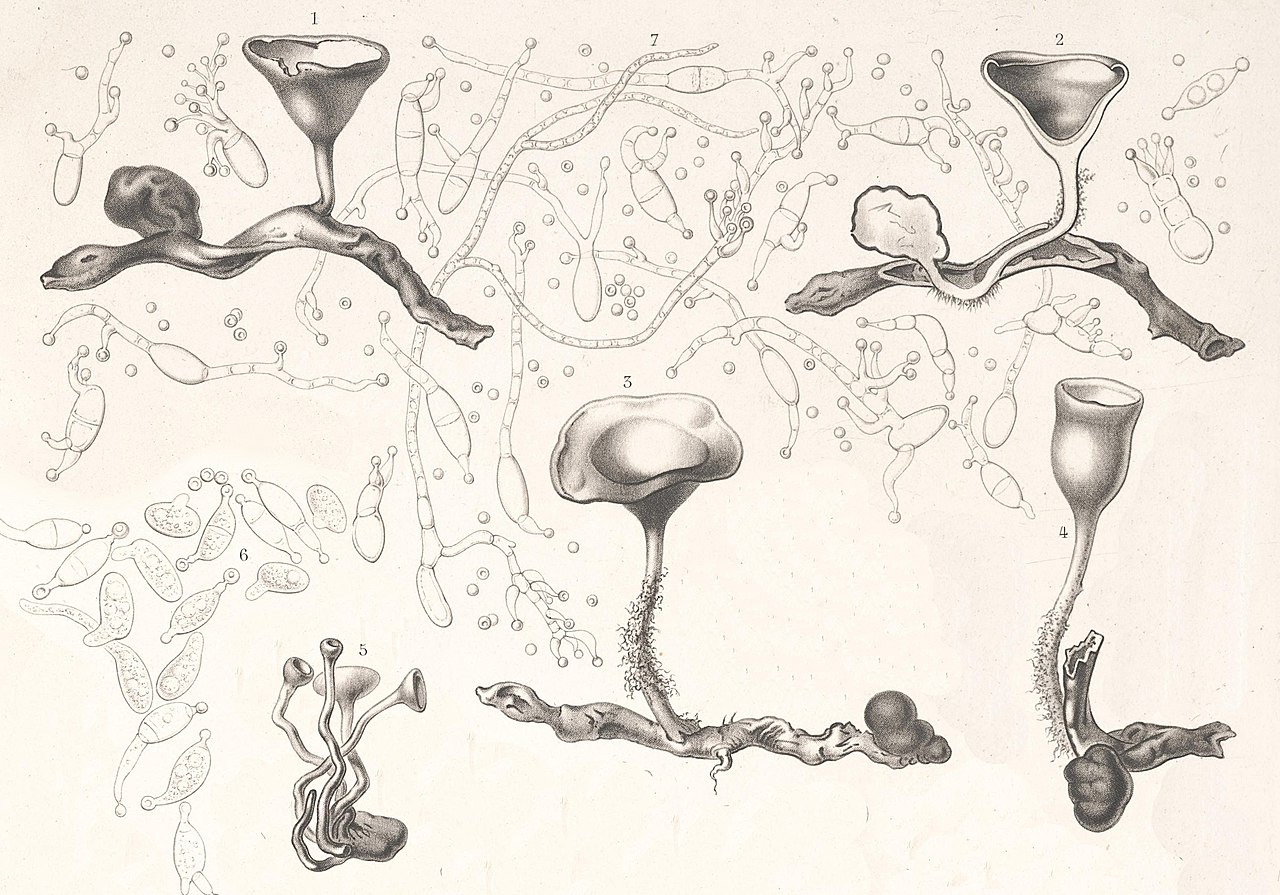
\includegraphics[width=\linewidth]{Figures/PezizaTuberosa.jpg}
%     \caption[Illustration of the fungus Dumontinia tuberosa.]{Illustration of the fungus Dumontinia tuberosa by physician, mycologist, and illustrator Charles Tulasne (1816–1884) in the book Selecta Fungorum Carpologia (1861–65). (Name of the original work: Peziza tuberosa parasite on Anemone nemorosa).}
%     \label{fig:figure-01}
% \end{figure}

% For the purpose of comparing or for other reasons, you can insert side-by-side figures using both the \verb|\begin{figure}| and \verb|\begin{subfigure}| environments. You can also refer to the sub-figure as \autoref{fig:figure-02.1} and \autoref{fig:figure-02.2}.

% \begin{figure}[!htpb]
%     \centering
%     \begin{subfigure}{0.45\textwidth}
%         \centering
%         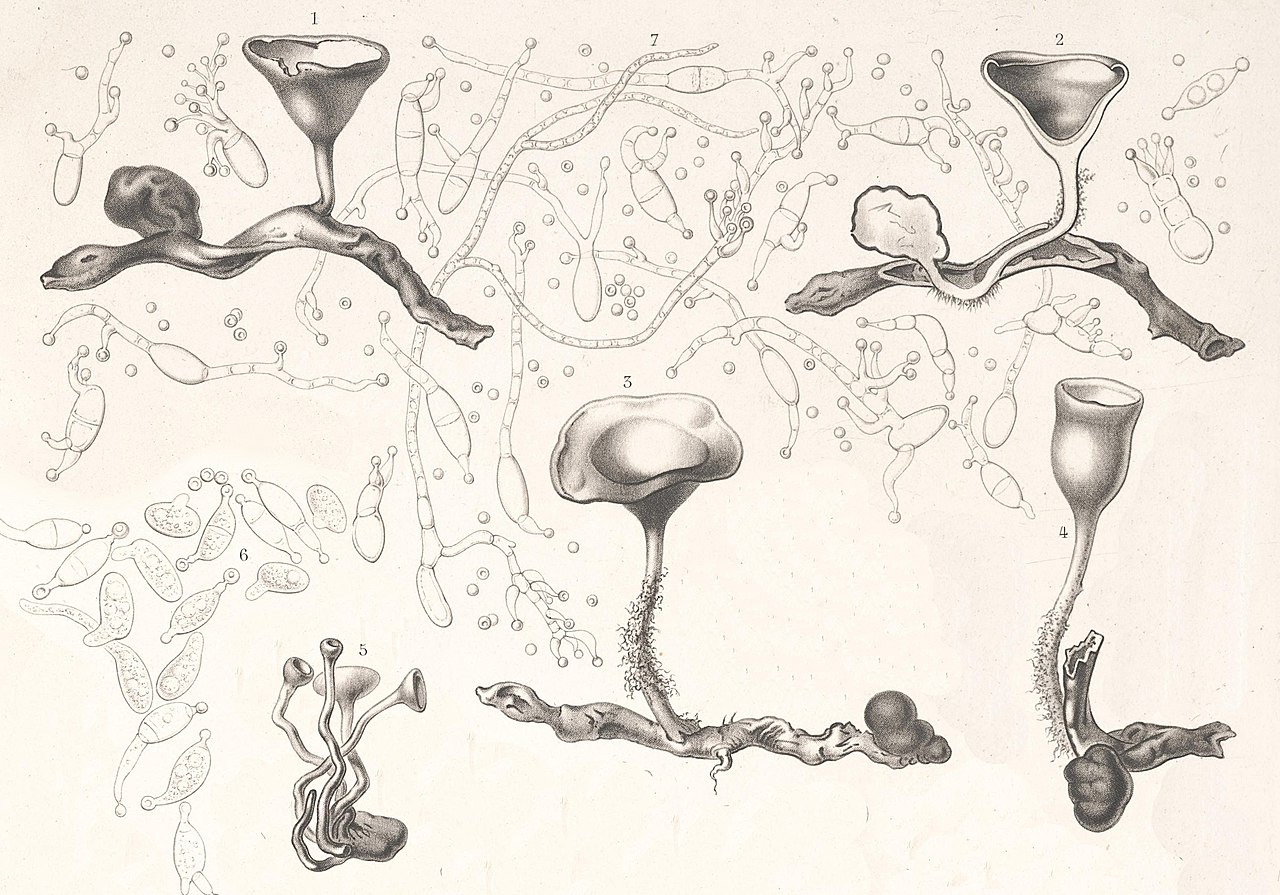
\includegraphics[width=0.9\textwidth]{Figures/PezizaTuberosa.jpg}
%         \caption{Caption for figure 1.}
%         \label{fig:figure-02.1}
%     \end{subfigure}
%     \hspace{.5cm} % Adjust the space as needed.
%     \begin{subfigure}{0.45\textwidth}
%         \centering
%         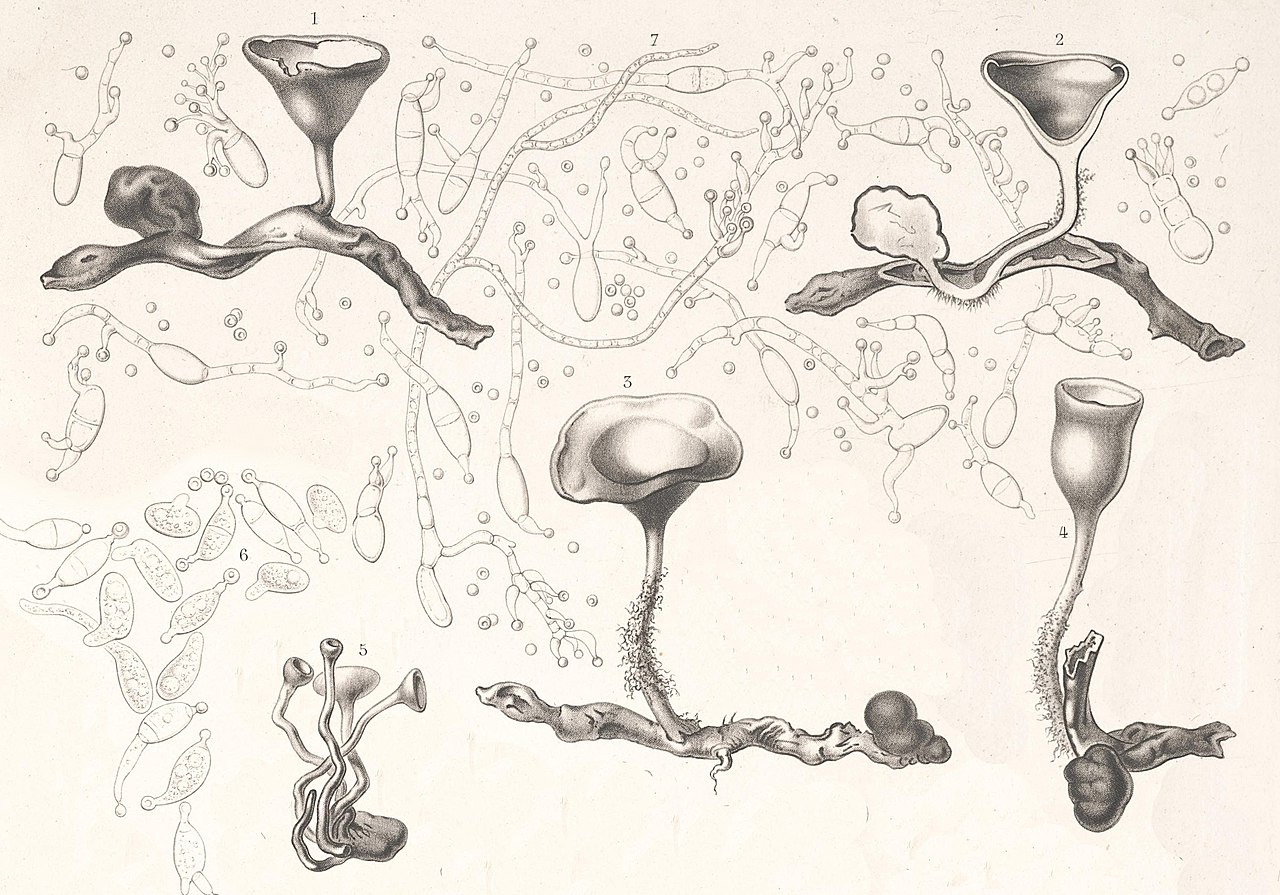
\includegraphics[width=0.9\textwidth]{Figures/PezizaTuberosa.jpg}
%         \caption{Caption for figure 2.}
%         \label{fig:figure-02.2}
%     \end{subfigure}
%     \caption{Overall caption of the figure.}
%     \label{fig:figure-02}
% \end{figure}

% \section{Tables}
% Tables are vital for presenting findings effectively. This chapter explores techniques for conveying information through tables using various template environments. Defining tables in \LaTeX\ seems complex, but this template simplifies the process.

% \begin{block}[tip]
% \textit{Prior to showcasing the different table environments, it's crucial to note that each one must be enclosed within a \texttt{\textbackslash begin\{table\}} environment. Additionally, it is recommended to utilise the \texttt{[!htpb]} float options for improved document placement. \textbf{This advice should be taken into consideration when positioning figures as well}.}
% \end{block}

% \subsection{Tabular Environment}
% The conventional \verb|\begin{tabular}| environment enables you to create a simple yet elegant table. \autoref{tab:table-01} is generated using a centering environment for added emphasis. It also incorporates the \verb|booktab| configuration for a more sophisticated table style.

% \begin{table}[!htpb]
%     \caption{A table showcasing the usage of the tabular environment.}
%     \label{tab:table-01}
%     \centering
%     \begin{tabular}{llc}
%         \toprule
%         \textbf{Header 01} & \textbf{Header 02} & \textbf{Header 03} \\ 
%         \midrule
%         Lorem Ipsum         & Pharetra Dolor    & $\checkmark$  \\
%         Amet Consectetuer   & Curabitur Aliquet & -             \\
%         Praesent Mauris     & Praesent Libero   & $\checkmark$  \\
%         \bottomrule
%     \end{tabular}
% \end{table}

% \subsection{Tabularx Environment}
% Employ the \verb|\begin{tabularx}| package to construct a table featuring automatically expanding multi-columns. To achieve this automatic behaviour for multi-columns, you can use the following environment: \verb|\begin{tabularx}{\textwidth}{lX}|, where \verb|X| is the column that will function as a multi-column. \autoref{tab:table-02} showcases the usage of the \verb|begin{tabularx}| environment.
% %Take note that we substitute \verb|X| in place of \verb|l| or \verb|c|, explicitly indicating that the column will function as a multi-column, occupying the entire available space.

% \begin{table}[!htpb]
%     \caption{A table showcasing the usage of the tabularx environment.}
%     \label{tab:table-02}
%     \begin{tabularx}{\textwidth}{lX}
%         \toprule
%         \textbf{Header 01} & \textbf{Header 02} \\ 
%         \midrule
%         Foo Bar Baz & Quisque cursus, metus vitae pharetra auctor, sem massa mattis sem, at interdum magna augue eget diam. \\
%         Ipsum Dolor & Vestibulum ante ipsum primis in faucibus orci luctus et ultrices posuere cubilia Curae; Curabitur aliquet quam id dui. \\
%         Dolor Sit & Phasellus condimentum elementum justo, quis interdum est sagittis ac. Vestibulum non arcu sit amet justo lobortis semper. \\
%         Amet Consectetuer & Integer nec odio praesent libero sed cursus ante dapibus diam sed nisi vestibulum non arcu. \\
%         Consectetuer Adipiscing & Nulla quis sem at nibh elementum imperdiet. Duis sagittis ipsum. Praesent mauris. \\
%         \bottomrule
%     \end{tabularx}
% \end{table}

% \subsection{Longtable Environment}
% At times, when dealing with exceptionally lengthy tables, it becomes necessary to split them across multiple pages. In \LaTeX, this can be achieved using the \verb|\begin{longtable}| environment. This environment is slightly more complex than others, as you need to define the header twice: once for the initial appearance of the table and again for when the table spans additional pages. This repeated header ensures the reader can correctly identify the columns on subsequent pages. Feel free to consult \autoref{tab:table-03} for a detailed demonstration of how the \verb|longtable| environment works.

% \begin{longtable}[c]{llll}
% \caption{A table showcasing the usage of the longtable environment.}
% \label{tab:table-03} \\
% \toprule
% \textbf{Names} & \textbf{E-Mails} & \textbf{Job/Role} \\ \midrule
% \endfirsthead
% %
% \multicolumn{4}{c}%
% {{\textit{\bfseries Table \thetable\ continued from previous page.}}} \\
% \toprule
% \textbf{Names} & \textbf{E-Mails} & \textbf{Job/Role} \\ \midrule
% \endhead
% %
% \bottomrule
% \addlinespace[1mm]
% \multicolumn{4}{r}%
% {{\textit{Continued on the next page.}}} \\
% \endfoot
% \bottomrule
% %
% \endlastfoot
% %
% Alice Johnson & alice.johnson@email.com & Project Manager \\
% Bob Thompson & bob.thompson@email.com & Data Analyst \\
% Charlie Davis & charlie.davis@email.com & Marketing Specialist \\
% David Miller & david.miller@email.com & QA Tester \\
% Emily White & emily.white@email.com & Graphic Designer \\
% Frank Martin & frank.martin@email.com & HR Coordinator \\
% Grace Turner & grace.turner@email.com & Financial Analyst \\
% Henry Lee & henry.lee@email.com & System Administrator \\
% Ivy Carter & ivy.carter@email.com & Customer Support \\
% Jack Wilson & jack.wilson@email.com & Frontend Developer \\
% Jane Reed & jane.reed@email.com & UX Designer \\
% Kevin Evans & kevin.evans@email.com & Product Manager \\
% Linda Adams & linda.adams@email.com & Accountant \\
% Mike Hill & mike.hill@email.com & Network Engineer \\
% Nina Garcia & nina.garcia@email.com & Business Analyst \\
% Oliver Smith & oliver.smith@email.com & Sales Representative \\
% Pamela Turner & pamela.turner@email.com & Legal Counsel \\
% Quincy Brown & quincy.brown@email.com & IT Consultant \\
% Rachel Moore & rachel.moore@email.com & Content Writer \\
% Samuel White & samuel.white@email.com & Research Scientist \\ 
% Amy Harris & amy.harris@email.com & Digital Strategist \\
% Brian Cook & brian.cook@email.com & Operations Manager \\
% Catherine Ross & catherine.ross@email.com & Brand Manager \\
% Daniel Green & daniel.green@email.com & Database Administrator \\
% Emma Taylor & emma.taylor@email.com & Social Media Manager \\
% Felix Carter & felix.carter@email.com & Compliance Officer \\
% Gloria Scott & gloria.scott@email.com & Procurement Specialist \\
% Harold Bennett & harold.bennett@email.com & DevOps Engineer \\
% Isla Cooper & isla.cooper@email.com & User Researcher \\
% James Black & james.black@email.com & Mobile App Developer \\
% Katie Brown & katie.brown@email.com & UI Designer \\
% Leo Perez & leo.perez@email.com & Scrum Master \\
% Megan Clark & megan.clark@email.com & Event Coordinator \\
% Nathan Ward & nathan.ward@email.com & Security Analyst \\
% Olivia Harris & olivia.harris@email.com & Corporate Trainer \\
% Paul King & paul.king@email.com & Territory Manager \\
% Queen Foster & queen.foster@email.com & Paralegal \\
% Rebecca Adams & rebecca.adams@email.com & Copy Editor \\
% Steven Martin & steven.martin@email.com & Robotics Engineer \\
% \end{longtable}

% \subsection{Complex Tables}
% Creating intricate tables in \LaTeX\ can be a somewhat challenging task. Therefore, we highly recommend using the \href{https://www.tablesgenerator.com/}{Table Generator}. With this tool, you can design your table with the desired style and then easily copy and paste it into your document. This approach simplifies the process and helps ensure the accurate representation of complex tables in your \LaTeX\ document. However, it's crucial to keep in mind that a table should be easily comprehensible for the reader and should not be overly complex. \textbf{The complexity of a table may impede understanding.} For example, \autoref{tab:table-04} presents a table with intricate details.

% \begin{table}[!htpb]
%     \caption{A table showcasing the usage of the complex tables.}
%     \label{tab:table-04}
%     \centering
%     \begin{tabular}{lcc}
%         \toprule
%         \multirow{2}{*}{\textbf{Component}} & \multicolumn{2}{c}{\textbf{Specifications}} \\
%         \cmidrule(lr){2-3}
%         & \textbf{Characteristic} & \textbf{Supported} \\
%         \midrule
%         \multirow{4}{*}{CPU} & Core Count (e.g., 8 Cores) & $\checkmark$ \\
%         & Clock Speed (e.g., 3.6 GHz) & $\checkmark$ \\
%         & Hyper-Threading & $\checkmark$ \\
%         & Integrated Graphics & - \\
%         \midrule
%         \multirow{4}{*}{GPU} & CUDA Cores (e.g., 5120) & $\checkmark$ \\
%         & Base Clock (e.g., 1.5 GHz) & $\checkmark$ \\
%         & Ray Tracing Support & $\checkmark$ \\
%         & Multi-GPU Support (SLI/CrossFire) & - \\
%         \midrule
%         \multirow{4}{*}{Memory} & Type (e.g., DDR5, GDDR6) & $\checkmark$ \\
%         & Capacity (e.g., 16 GB) & $\checkmark$ \\
%         & Memory Bandwidth (e.g., 448 GB/s) & $\checkmark$ \\
%         & ECC Support & - \\
%         \midrule
%         \multirow{3}{*}{Motherboard Features} & PCIe 5.0 Support & $\checkmark$ \\
%         & Wi-Fi 6E & $\checkmark$ \\
%         & Thunderbolt 4 & - \\
%         \bottomrule
%     \end{tabular}
% \end{table}

% \section{Lists}
% Creating lists in \LaTeX\ is straightforward, offering various options to suit your needs. You can generate a bullet list using \verb|\begin{itemize}|, or opt for a numbered list with \verb|\begin{enumerate}|. Below is an example with the \verb|\begin{itemize}| environment.

% \begin{itemize}
%   \item List entries start with the \verb|\item| command.
%   \item Individual entries are indicated with a black dot, a so-called bullet.
%   \item The text in the entries may be of any length.
% \end{itemize}

% As mentioned earlier, you can generate a numbered list using the \verb|\begin{enumerate}| environment. Here is an example:

% \begin{enumerate}
%   \item Items are numbered automatically.
%   \item The numbers start at 1 with each use of the \verb|enumerate| environment.
%   \item Another entry in the list.
% \end{enumerate}

% You can also nest list entries by creating a list inside another list of the same type. Here is an example:

% \begin{enumerate}
%     \item First level item
%     \item First level item
%     \begin{enumerate}
%         \item Second level item
%         \item Second level item
%     \begin{enumerate}
%         \item Third level item
%         \item Third level item
%     \end{enumerate}
%     \end{enumerate}
% \end{enumerate}

% \begin{block}[tip]
% \textit{Please note that the labels change automatically regardless of the environment being the same for every list. \textbf{This demonstrates that there's no need to worry about changing the environment for something different.}}
% \end{block}

% You can also modify the label of your list to something entirely different that suits your needs. To accomplish this, insert a new \verb|\item| and enclose your desired label in square brackets. For example, \verb|\item[!]| will result in an exclamation point as your new label. Below are some examples of modified labels.

% \begin{itemize}
%   \item This is my first point
%   \item Another point I want to make 
%   \item[!] A point to exclaim something!
%   \item[$\blacksquare$] Make the point fair and square.
%   \item[] A blank label?
% \end{itemize}

% Finally, you can create a description list. Unlike having a bullet point or a numbered label, a description list enables you to use custom descriptions that suit your list. In the example below, there are three \verb|\item| entries: one without a label, and two with descriptions.

% \begin{description}
%     \item[Item 1:] This is the first item with a description.
%     \item[Item 2:] Another item with a different description.
%     \item An item without a specific label.
% \end{description}

% \section{Code Listings}
% At times, you may want to include source code from your programs and applications within your document. To achieve this, you can use two nested environments: \verb|\begin{listing}| to create a listing with both caption and label, and \verb|\begin{minted}| for code highlighting. \autoref{listing:c-code} provides an example of a source code in C.

% \begin{listing}[!htpb]
% \caption{Hello world in C.}
% \label{listing:c-code}
% \begin{minted}{c}
% #include <stdio.h>
% int main() {
%   printf("Hello, World!"); /* printf() outputs the quoted string */
%   return 0;
% }
% \end{minted}
% \end{listing}

% The code mentioned above was inserted into the document. However, an alternative approach is to input your code from an external file. To do so, you just need to use the command \verb|\inputminted{CODE_LANGUAGE}{FILE}|. Of course, you should place that command inside of the \verb|\begin{listing}| environment. \autoref{listing:haskell-code} illustrates an example of Haskell source code that has been input from an external file.

% \begin{listing}[!htpb]
% \caption{Factorial in Haskell.}
% \label{listing:haskell-code}
% \inputminted{haskell}{Code/Factorial.hs}
% \end{listing}

% In some cases, when you simply want to highlight a specific command, it's recommended not to use \verb|listing| or \verb|minted|. Instead, you should utilise the \verb|\verb| command for inline highlighting or the \verb|\begin{verbatim}| environment for longer sections of highlighted code. An example of a lengthy \verb|verbatim| section is provided below, demonstrating how to create a \verb|listing| with an input code:

% \begin{verbatim}
% \begin{listing}[!htpb]
%     \inputminted{CODE_LANGUAGE}{FILE}
%     \caption{TEXT}
%     \label{TEXT}
% \end{listing}
% \end{verbatim}

% Sometimes it is necessary to display longer code that occupies more than one page. For this purpose, please use the environment \verb|\begin{longlisting}|. This environment will easily break your code into multiple pages for better readability without you worrying about the size of your code. An example is shown below in \autoref{listing:lisp-code}.

% \begin{longlisting}
% \caption{A sample of functions in Lisp.}
% \label{listing:lisp-code}
% \begin{minted}{lisp}
% (defun factorial (n)
%  "Calculate the factorial of a number."
%  (if (zerop n)
%      (* n (factorial (1- n)))))

% (defun fibonacci (n)
%  "Calculate the nth Fibonacci number."
%  (cond ((zerop n) 0)
%        ((= n 1) 1)
%        (t (+ (fibonacci (1- n)) (fibonacci (- n 2))))))

% (defun gcd (a b)
%  "Calculate the greatest common divisor of a and b."
%  (if (zerop b)
%      a
%      (gcd b (mod a b))))

% (defun primes-up-to (limit)
%  "Return a list of all prime numbers up to LIMIT."
%  (let ((primes '()))
%    (loop for i from 2 to limit
%          unless (some (lambda (p) (zerop (mod i p))) primes)
%          do (push i primes))
%    (nreverse primes)))

% (defun example-function (x)
%  "An example function to demonstrate Lisp capabilities."
%  (let ((result (list (factorial x)
%                      (fibonacci x)
%                      (gcd x 10)
%                      (primes-up-to x))))
%    (format t "Factorial of ~A: ~A~%" x (factorial x))
%    (format t "Fibonacci of ~A: ~A~%" x (fibonacci x))
%    (format t "GCD of ~A and 10: ~A~%" x (gcd x 10))
%    (format t "Primes up to ~A: ~A~%" x (primes-up-to x))
%    result))

% (example-function 10)
% \end{minted}
% \end{longlisting}

% \section{Equations}
% When writing equations and other mathematical expressions, \LaTeX~is a powerful and versatile tool. You can enter a formula in inline mode using the environment \verb|\(FORMULA\)| or use \verb|\begin{equation}| to display it in ``math mode'' with numbering. If you prefer not to display the equation number, you can use the environment \verb|\[FORMULA\]|.

% \vspace{.875em}
% \textbf{Example:} In physics, the mass-energy equivalence is expressed by the equation \(E=mc^2\), discovered in 1905 by Albert Einstein. In natural units ($c = 1$), the formula (\ref{eq:equation-01}) expresses the identity:

% \begin{equation}
% \label{eq:equation-01}
% E=m
% \end{equation}

% \textbf{Example:} Below is a equation -- \textit{without numbering} -- for the regularised loss function in supervised learning, combining the average prediction loss over the training dataset and an $L_2$ regularisation term to prevent overfitting:

% \[
% \mathcal{L}(\boldsymbol{\theta}) = \frac{1}{N} \sum_{i=1}^{N} \ell(y_i, f(\mathbf{x}_i; \boldsymbol{\theta})) + \lambda \|\boldsymbol{\theta}\|_2^2
% \]

% Equations can be a bit challenging to create, so we advise using an online editor, like the \href{https://latexeditor.lagrida.com/}{LaTeX Equation Editor}. Simply build your formulas there and copy and paste them into your document, either inline or in a math block, as shown above.

% \section{Footnotes}
% Sometimes it is important to present information that is not central to the main text in a footnote. In \LaTeX\, this can be easily achieved using the command \verb|\footnote{TEXT}|. The text will appear at the bottom of the page\footnote{This is a simple footnote.}.

% If you want to use footnotes within tables, it is best to reconsider, as \LaTeX\ does not provide an easy way to handle them. Instead, you can place a ``*'' wherever you want the footnote reference to appear. Then, below the table \textbf{but before ending the table environment}, place the ``*'' along with the footnote text. This will create a similar footnote, but it will appear below the table rather than at the bottom of the page.


}